
\documentclass[a4paper, 11pt]{article}

\usepackage{verbatim}
\usepackage{pdfpages}
\usepackage[T1]{fontenc}
\usepackage{titling}
\usepackage{amsmath}
\usepackage{siunitx}
\usepackage{amsfonts}
\usepackage{graphicx}
\usepackage{mathtools}
\usepackage[includeheadfoot,margin=23mm]{geometry}
\usepackage{multirow}
\usepackage{siunitx}
\usepackage{mhchem}
\usepackage{xfrac}
\usepackage{epstopdf}
\usepackage{float}
\makeatletter
\newcommand{\sectionauthor}[1]{}
\makeatother
\usepackage[bottom]{footmisc}
\usepackage{helvet}
\renewcommand{\familydefault}{\sfdefault}

\usepackage{chngcntr}
\counterwithin{figure}{section}

\usepackage{caption}
\usepackage{subcaption}

\usepackage{gensymb}

\usepackage{setspace}
\doublespacing

\usepackage{fancyhdr}
\pagestyle{fancy}
\cfoot{\fancyplain{}{\thepage}}

\usepackage{fancyhdr}
\pagestyle{fancy}
\fancypagestyle{wojciech}{
	\fancyhead{} % clear all header fields
	\lhead{\leftmark }
	\rhead{Wojciech Dziwulski}
	\cfoot{\thepage}
}

\usepackage{fancyhdr}
\pagestyle{fancy}
\fancypagestyle{alex}{
	\fancyhead{} % clear all header fields
	\lhead{\leftmark }
	\rhead{Alexander Dwornik}
	\cfoot{\thepage}
}

\usepackage{fancyhdr}
\pagestyle{fancy}
\fancypagestyle{judah}{
	\fancyhead{} % clear all header fields
	\lhead{\leftmark }
	\rhead{Judah Rand}
	\cfoot{\thepage}
}

\usepackage{fancyhdr}
\pagestyle{fancy}
\fancypagestyle{john}{
	\fancyhead{} % clear all header fields
	\lhead{\leftmark }
	\rhead{John Boyer}
	\cfoot{\thepage}
}

\usepackage{fancyhdr}
\pagestyle{fancy}
\fancypagestyle{ref}{
	\fancyhead{} % clear all header fields
	\lhead{\leftmark }
	\rhead{}
	\cfoot{\thepage}
}


\usepackage{titlesec}
\setcounter{secnumdepth}{4}
\titleformat{\paragraph}
{\normalfont\normalsize\bfseries}{\theparagraph}{1em}{}
\titlespacing*{\paragraph}
{0pt}{3.25ex plus 1ex minus .2ex}{1.5ex plus .2ex}
\usepackage{gensymb}



\renewcommand{\headrulewidth}{0.5pt}

\numberwithin{equation}{section}
\usepackage[numbered, framed]{matlab-prettifier}

\lstset{
	style              = Matlab-editor,
	escapechar         = ",
	mlshowsectionrules = true,
	tabsize            = 2,
}

\graphicspath{{Images/}}

\setlength{\droptitle}{-8em}

\title{Saving Oneself \\ \large Third Year Project}

\author{\textbf{John Boyer, Alexander Dwornik, Wojciech Dziwulski, Judah Rand}}

\date{}

\begin{document}
	
	\clearpage
	\maketitle
	\thispagestyle{empty}
	\begin{abstract}
		
		It is currently impossible to extract and store the information that a human brain accumulates over one's lifetime. Our research proposes an extensive pipeline to retrieve the locations of synapses, therefore providing us with the necessary information to map out an individual's connectome. Ethical issues inevitably arise as this process requires the termination of a human life. This is necessitated by the need for preservation, to prevent degradation of tissue and prepare for both storage and sectioning. The size of the human brain has required us to develop a new tool for the sectioning pipeline to work alongside those already proven in use throughout the neuroscience community. Further chemical processes will be needed to prepare the sample for imaging, each comes with benefits however the BROPA method is shown to be the best option. A clear record of techniques for high resolution imaging of brain tissue provides a reference for future endeavours and examines both the benefits and failings of each individually. Our current chosen technique is fully assessed for its suitability along with possible future developments and a small discussion with the manufacturer on viability. Various data organisation frameworks and querying tools proceed to be presented and contrasted. These are then used to estimate the storage requirement for one human brain. A range of machine learning techniques are described and compared. This justifies the choice of bagged tree ensembles in conjunction with hand-designed features for the image segmentation. The corresponding hardware requirements and running time efficiency are also presented. Finally, a detailed business case will consider the full project cost and sources of investment.
		
	\end{abstract}
	
	\newpage
	
\includepdf[]{DeclarationofAuthorship3YP}
	\newpage
	
\includepdf[]{DeclarationofAuthorship3YP}
	\newpage
	
\includepdf[]{DeclarationofAuthorship3YP}
	\newpage
	
\includepdf[]{DeclarationofAuthorship3YP}
	
	\newpage
	\pagenumbering{roman}
	\tableofcontents 
	
	
	\newpage
	\pagenumbering{arabic}
	
	
	\clearpage
	
	\pagestyle{judah}
\section{Introduction}
\label{intro}
The aim of this report is to outline the design and facilities needed for a system capable of capturing the information in a human brain in its entirety, thus avoiding information-theoretic death. This means that future technologies will be able to infer the original state of our client's brain, including their memories and personality, effectively reanimating them.

\subsection{Anatomy of the Brain}
The brain is by far the most complex organ which we, as human beings, possess. It is fundamental to who we are and how we perceive the world around us. Our understanding of how this immensely complex structure works is still limited but is rapidly developing. It was in fact only in the latter half of the 18th century that Luigi Galvani observed the importance of electrical signals in nerves. Since then our knowledge of the structures contained within the brain have developed immensely.

The brain is made up of two types of tissue, grey matter and white matter. Grey matter accounts for between 50-60\% of the brain's volume \cite{luders2002brain}. This tissue contains dendrites, axon terminals and cell bodies of neurons, as a result this is where most synaptic connections are made. White matter accounts for the other 40-50\% of the brain, this tissue is made up of myelinated axons. Until recently white matter has been considered to be mostly passive, simply acting as an information highway between various part of the brain, however, it is beginning to be understood that white matter also plays a crucial part in learning and continues to develop well into one's life \cite{fields2008white}.

Neurons (Figure \ref{neuron}) are a key building block that make up the brain. Their main structures are axons and dendrites. There is one axon per neuron which transmits signals away from the cell body to other neurons and for the presynaptic side of a synapse. There are, on the other hand, normally many dendrites per neuron which form the postsynaptic density and receive signals from other cells to pass onto the cell body. There are somewhere between 19-23 billion neurons in the brain \cite{parsell2009steven} and each of these neurons connects to thousands of others via synapses. 


\begin{figure}[H]
	\centering
	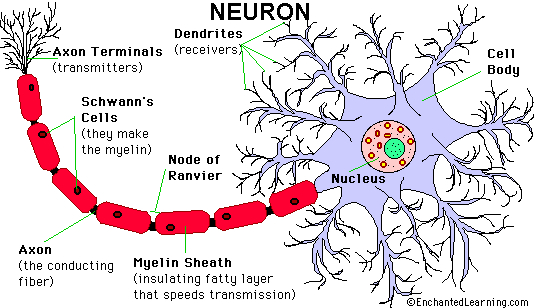
\includegraphics[width = 0.6\textwidth]{Neuron.jpg}
	\caption[]{The anatomy of a neuron\footnotemark}
	\label{neuron}
\end{figure}
\footnotetext{http://www.enchantedlearning.com/subjects/anatomy/brain/gifs/Neuron.GIF [Accessed 14/04/16]}


These synapses transfer signals between neurons either by chemical neurotransmitters or electrical impulses. Figure \ref{synapse} shows an example of a chemical synapse. When one of these chemical synapses is excited, the axon terminal releases chemical neurotransmitter from its synaptic vesicles. This transmitter diffuses across the synaptic cleft and interacts with the neurotransmitter receptors on the postsynaptic density on the dendritic spine of another neuron. This means that chemical synapses have an inherent delay in transmission and are unidirectional.

\begin{figure}[h]
	\centering
	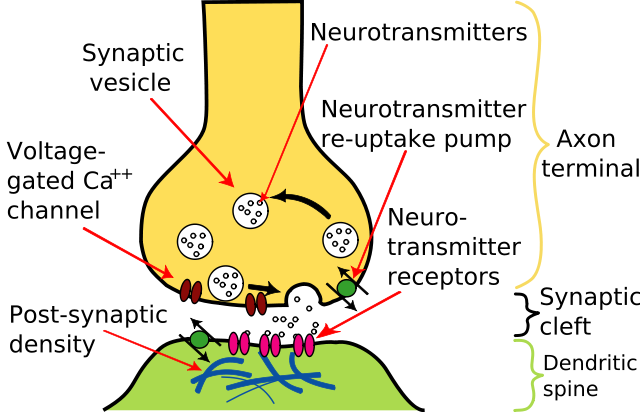
\includegraphics[width=0.55\textwidth]{synapse}
	\caption[]{Example of a chemical synapse\footnotemark}
	\label{synapse}
\end{figure}
\footnotetext{http://www.cs.mcgill.ca/rwest/link-suggestion/wpcd\_2008-09\_augmented/images/666/66667.png.htm\#filehistory [Accessed 14/04/16]}

Electrical synapses are much less common but no less crucial to the functioning of a brain. They transmit their signals by allowing ionic current to directly flow between the pre- and postsynaptic neurons. This allows for a much faster signal transmission as well as the potential for a bidirectional flow of information. Both chemical and electrical synapses can be identified and distinguished in electron micrographs as shown in Figure \ref{chemical_vs_electrical}.

\begin{figure}[h!]
	\centering
	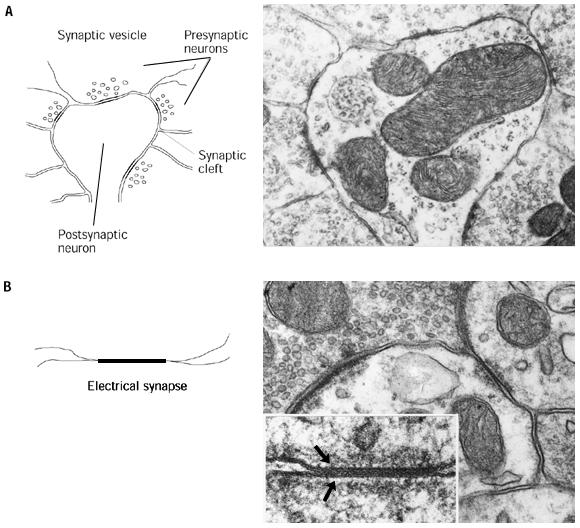
\includegraphics[width=0.55\textwidth]{chemical_vs_electrical}
	\caption[]{Comparison of chemical and electrical synapses\footnotemark}
	\label{chemical_vs_electrical}
\end{figure}
\footnotetext{http://163.178.103.176/CasosBerne/1aFCelular/Caso4-2/HTMLC/CasosB2/Receptor/Ch6.html [Accessed 14/04/16]}

Another significant cell type is glial cells, which outnumber neurons by about three to one \cite{glial_number}. Originally glial cells were thought to simply provide support and insulation for neurons, hence glial is Greek for "glue". However, research into the function of glial cells has been limited and therefore the understanding of the function of these cells is still developing. Recently evidence of neuron-glial communication has emerged \cite{fields2002new} and it is becoming increasingly clear that these non-neuronal cells have a role to play in the movement of information through the brain.

\subsection{The Connectome}
\label{connectome}
It has been shown that changes in synaptic connections is fundamental to learning and memory \cite{mayford2012synapses}\cite{rogerson2014synaptic}. These changes include the strengthening or weakening of existing synapses, the creation of new connections or even the pruning of existing connections. This suggests that a person's memories, skills and experiences are all stored within the neuronal circuit contained within their skull; therefore, this circuit defines `who they are'. If this structure could be captured in its entirety, it may be possible in the future to recreate the neural circuit and reanimate the person's mind. This neural map is known as the `connectome'.

It is, however, also true that the mechanism of consciousness is not understood, with some experts believing that glial cells play a much more fundamental roll in human conscientiousness and intelligence than has previously been thought. For example, links have been made between the intelligence of a species and the size and number of astroglia with humans having the most and biggest astroglia \cite{koob2009root}. Despite this, we feel that the best way to proceed with what has until now been humanity's fantasy of immortality is to obtain a complete human connectome. It is also important to us that the potential information contained in the glial cells of the brain are not forever lost as it is foreseeable that this information may in fact be required for complete reconstruction. For this reason, the pipeline outlined in this report strives to preserve this information either through storage of the physical brain itself or of the images obtained of the brain.

Connectomes of much simpler species have already been completed, one such example is \textit{Caenorhabditis elegans}. This worm's connectome consists of only 302 neurons with 8,963 synaptic connections\cite{varshney2011structural}. Even this small connectome was a mammoth undertaking, every structure which appeared in the electron micrograph of worm's central nervous system had to be labelled manually. From this it is clear that producing a similar map for a human brain with approximately 1,000 trillion synapses %REFERENCE 
seems impossible. However, with the use of new and continually evolving technology and cutting edge segmentation algorithms this report hopes to outline a method which would make such an endeavour possible.  

%Alex D's Report

\newpage

\clearpage

\pagestyle{alex}

\section{Chemical Preparation}
\subsection{Introduction}

This project requires a method to be developed for scanning brain tissue to a sufficiently high enough resolution that enables neuronal connection detection and their associated strengths. In order to achieve this, the samples obtained via electron microscopy, must be chemically prepared to ensure the best possible chance of neural detection as well as maintaining and protecting the state of the brain after death. 

The initial challenge is to deal with the two stage chemical decomposition process (autolysis and putrefaction) which begins after the heart stops beating and the brain is removed from the body \cite{SoilAnalysisinForensicTaphonomy}. Autolysis begins with the cells releasing digestive enzymes from their lysosomes into the cytoplasm. These digestive enzymes begin breaking down the structures within the cell which eventually leads to a breakdown of the entire cell structure. Putrefaction then commences, as a result of the proteins decomposing, leading to a breakdown of cohesion between tissues. This ultimately leads to further destruction of the cell structure. This process is additionally accelerated by bacterial contamination. Clearly both of these chemical processes result in the degrading of cell integrity, making synapse detection impossible if left unchecked. Therefore, the chemical preparation process must take into account these decomposing chemical reactions. 

The second issue is the physical deformation of the brain after its removal from the body. The untreated brain is extremely soft, having a gel-like consistency with a low stiffness. This could be easily altered or damaged during or after removal. When investigating the effects of strain on brain tissue, it was found that at different strain rates a linear, viscoelastic model of brain tissue was not appropriate for modelling brain tissue deformation even for moderate strains. This clearly demonstrates the importance of using a fixative, in order to ensure the brain is not altered physically before imaging \cite{Miller2002483} \cite{Miller20001369}. Another reason for using a fixative is to minimise cell loss when sectioning the brain into smaller samples. 

The final key issue relates to the imaging of the brain. Without clear interaction between the focused beam of electrons in the SEM microscope and atoms within the sample, together with poor contrasting raw data, the image produced will not contain enough contrast. As a result, the algorithms used to detect synapses will yield poor results. Therefore, the sample must be stained with a solution of high density metal ions in order to increase electron interaction to provide greater contrasting images. \cite{HeavyMetalsWatson}.

In conclusion, chemical preparation is required in order to stop the physical and chemical processes from distorting and destroying the brain and the synapse located within it. In order to combat this, the brain will require fixation, staining, dehydration and embedding, as outlined in numerous reports relating to the preparation for SEM imaging \cite{wholemousebrain2012} 
\cite{Knott2011}. The fixation will ensure the structural integrity of the sample as well as minimising loss of cells when sectioning the brain. This will minimise the degradation of the brain after death. The staining using heavy metal ions will increase the contrast within the sample, improving the likelihood of detection within the segmentation section of the process. Dehydration is required to improve the clarity of images produced whilst embedding hardens the sample further. 


\subsection{Fixation}

In order to maximize the probability of fixing the brain in the same state post mortem, the fixation process must be carried out as soon as possible due to the irreversible damage that begins to occur after the patient dies. One paper found that the optimal period for fixation occurred when the time between the start of the fixation process and post-mortem was less than 12 hours \cite{Beach1987183}. 

The fixation process itself relies on diffusion via concentration gradients. The closer the fixation solution can be applied to the target cells and the stronger the concentration of the solution, the better the fixation process in terms of speed and uniformity. There are two recognised fixation methods - immersion and perfusion.

\subsubsection{Immersion}

The method of immersion works by slicing the brain sample into \SI{1}{\centi\metre} thick coronal sections \cite{Beach1987183} which are then immersed in a fixative solution which diffuses into the brain. The issue with this technique is that it only works well for small pieces of tissue. With larger samples, the fixative does not reach all of the tissue areas at the same rate, with the time required to diffuse chemicals into the brain theoretically scaling quadratically with brain mass. Another issue with this technique arises when the sample is sliced into \SI{1}{\centi\metre} thick coronal sections \cite{Beach1987183} and the cells suffer from hypoxia resulting in autolysis and putrefaction occurring before the fixative completely diffuses into all cells. Finally, as the brain has not already been fixated, sectioning it would result in further damage to the sample. For these reasons, we shall be using the perfusion method to deliver the fixative to the brain. 

\subsubsection{Perfusion}

This method uses the humans' natural vascular network to quickly access all areas within the brain \cite{AnimalPerfusion65}. The clear advantage perfusion offers over immersion is the speed and uniformity of the process, due to every cell being located within \SI{50}{\micro\metre} - \SI{100}{\micro\metre} of a capillary \cite{BiologyoftheCell}. When testing the two methods the immersion process penetration was limited to a depth of \SI{1} - \SI{2}{\milli\metre} \cite{Beach1987183} from the surface of the brain slice (\SI{1}{\centi\metre} thick). In contrast, staining density in perfusion-fixed brains was relatively homogeneous and of high quality. The paper also stated that when studying the brain post fixation, the perfused brain displayed more uniform staining throughout the sections compared with the immersed brains \cite{Beach1987183}. 

\newpage

\clearpage

\pagestyle{judah}

\subsubsection{Ethical \& Legal Concerns}
\label{ethics}

It is important to note that some of the discussed methods of preservation traditionally involve ending the subject's life while under anaesthesia. This includes any of the methods which require transcardial perfusion. This is perfectly acceptable when studies are being conducted on laboratory bred animals, however, in all Western countries deliberately ending a healthy individual's life is considered murder. In some countries, such as Switzerland, euthanasia is legal in some cases. Table \ref{euthanasia_table} lists European countries where euthanasia is legal.

\begin{table}[H]
	\centering
	\begin{tabular}{|l|l|}
		\hline
		\textbf{Country} & \textbf{Type of Euthanasia Legal} \\ \hline
		Belgium & Active \\ \hline
		Germany & Passive \\ \hline
		Holland & Active \\ \hline
		Luxembourg & Active \\ \hline
		Sweden & Passive \\ \hline
		Switzerland & Passive/Assisted suicide \\ \hline
	\end{tabular}
	\caption{List of European countries where euthanasia is legal}
	\label{euthanasia_table}
\end{table}

There are also very strict criteria which must be filled in order for euthanasia to be approved. In countries where euthanasia is legal these include:
\begin{itemize}
	\item The person has made an active and voluntary request to end their life.
	\item It is thought that they have sufficient mental capacity to make an informed decision regarding their care.
	\item It is agreed that the person is suffering unbearably and there is no prospect for an improvement in their condition.
\end{itemize} 

The law distinguishes between voluntary, non-voluntary and involuntary euthanasia. In all cases, for our purposes, any client would be going through the procedure of their own free will and so any euthanasia would be of a voluntary nature. There is also an additional legal distinction between active and passive euthanasia. While active euthanasia allows for the administration of lethal substances of forces whereas passive euthanasia only allows for the withholding of treatments which are required for the survival of the patient \cite{rachels1975active}.

Therefore, traditional perfusion methods would have to take place in countries in which active euthanasia is legal and on an individual who fulfils the legal requirements. This means that it is likely that the individual would have to have a terminal illness. This is undesirable as it severely limits the pool of possible participants. Belgium has the most progressive view of euthanasia of any European country and it is here that it is most likely that legal approval will be granted to perform a traditional transcardial perfusion on a human.

\newpage

\clearpage

\pagestyle{alex}

\subsubsection{Surgical plane of Anaesthesia}
	\label{Anaesthesia}


The chemical preparation process that we are using is based on the method described in \cite{Aldehyde_stabilized_cryopreservation} with the main difference being the volume of solutions used. 
Perfusion begins by putting the subject in a surgical plane of anaesthesia. A mixture of ketamine and xylazine is administered via intraperitoneal injection (for ketamine up to $\SI{80}{\milli\gram}$ per kg of body weight and for xylazine up to $\SI{10}{\milli\gram} $ per kg of body weight) \cite{AnimalPerfusion65}. 

Data suggests that the average man in the UK weighs \SI{86.3}{\kilo\gram} \footnote{http://www.bbc.co.uk/news/uk-11534042x [Accessed 05/03/2016]}, therefore the maximum administered dosage for an average UK man would be $\SI{80}{\milli\gram\per\kilo\gram}\times\SI{83.6}{\kilo\gram}=\SI{6.69}{\gram}$ of ketamine and $\SI{10}{\milli\gram\per\kilo\gram}\times\SI{83.6}{\kilo\gram}=\SI{0.84}{\gram} $ of xylazine. This can be altered depending on the patient. After being induced with the ketamine and xylazine, the subject should be kept at an appropriate surgical plane of anaesthesia using \SI{1}\% - \SI{5}\% isoflurane with \SI{100}\% oxygen by mask \cite{Aldehyde_stabilized_cryopreservation}.

Once the subject is in a surgical plane of anaesthesia a trained surgeon must perform a bilateral carotid cannulation operation. In order to successfully perfuse all cells within the brain, the surgeon will need to connect the ventricular assist device to the main arteries and veins located in the brain. The brain receives blood from two sources: the internal carotid arteries, which arise at the point in the neck where the common carotid arteries bifurcate, and the vertebral arteries \cite{BloodSupplyotheBrain}. However, the vertebral arteries feed into the internal carotids via the basilar artery. Another study showed that the internal and contralateral jugular veins are the main drainage vessels for blood leaving the brain \cite{Doepp2004}. This clearly suggests that in order to completely perfuse the brain, the ventricular assist device should be connected to both common carotid arteries as inputs and the internal jugular veins as outputs. 

\begin{figure}[h]
\centering
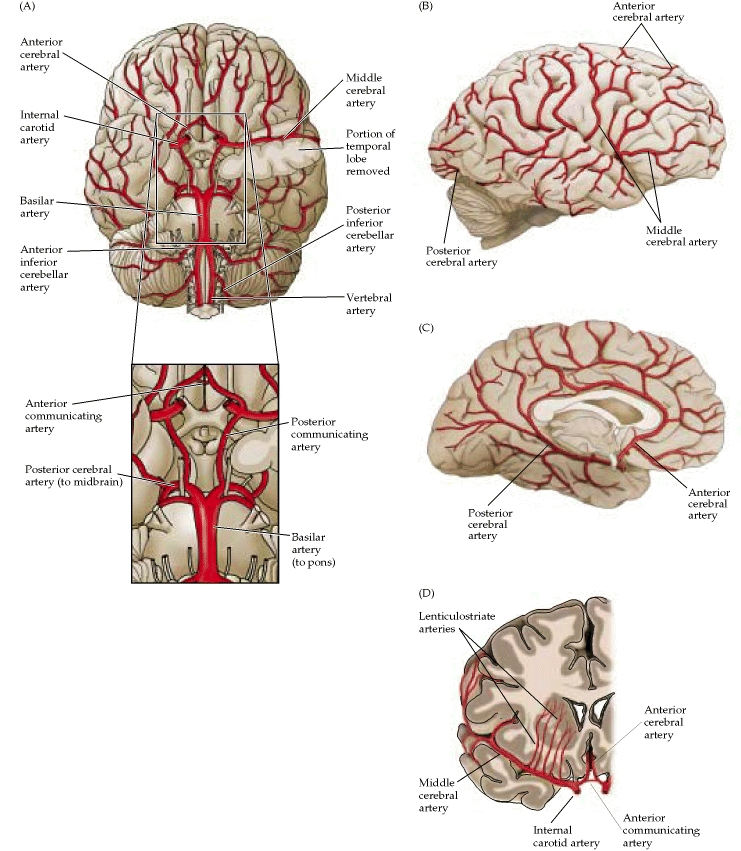
\includegraphics[width=0.70\textwidth]{Brain_blood_flow.jpg}
\caption{\label{fig:Brain_Flow}The major arteries of the brain \cite{BloodSupplyotheBrain}}
\end{figure}

\subsubsection{Washout Solution}

The blood washout solution (Table \ref{washoutsolution}) should have a pH similar to that of the blood it is replacing, average \SI{7.35} - \SI{7.45}{pH}\footnote{http://www.medicinenet.com/script/main/art.asp?articlekey=10001 [Accessed 19/3/2016]}, in addition to being well oxygenated (achieved by bubbling \ce{O2} through the solution for one hour before use) in order to prevent hypoxia and brain damage. This washout solution should be pumped around the blood stream via a Millipore \SI{0.22}{\micro\meter} filter using a manual Cephalon perfusion machine which acts as an artificial heart \cite{pulsatilemachineperfusion}. Healthy blood pressure is deemed to be 120mmHg over 80mmHg,\footnote{http://www.bloodpressureuk.org/BloodPressureandyou/Thebasics/Whatisnormal [Accessed 05/03/2016]} and hence the perfusion machine should output the washout solution, as well as other solutions at this rate (120/80mmHg) to ensure complete fixation. Any significant variation from this target pressure could cause irreversible damage to brain cells.

\begin{table}[H]
\centering

\begin{tabular}{|l|l|}
\hline
\textbf{Chemical} & \textbf{Concentration} \\ \hline
PBS 10x Concentrate & 100.00 mL/L \\ \hline
Ketamine & 5.40 mL/L \\ \hline
Sodium Heparin & 0.50 mL/L \\ \hline
Euthasol & 0.35 mL/L \\ \hline
\end{tabular}
\caption{Composition of phosphate-buffered saline (PSB) blood washout solution \cite{Aldehyde_stabilized_cryopreservation}}
\label{washoutsolution}
\end{table}

\paragraph{Washout Method}

After undergoing a general anaesthesia, the patient is maintained on a surgical plane. A bilateral carotid cannulation should be performed as follows:

\begin{enumerate}
\item The surgeon should make an incision in the neck in order to expose the carotids and dissect free the surrounding tissue. 
\item Ligatures should be looped loosely around both common carotid arteries. 
\item The left exposed carotid should be cut and a low-flow cannula should be inserted immediately.
\item Perfusion of the washout solution should begin at 120/80mmHg.
\item Ipsilateral jugular vein should be cut and connected to the input of the manual Cephalon perfusion machine.
\item The process should be repeated on the right carotid and contralateral jugular vein.
\item The blood washout solution should be run for 20 minutes, \cite{Aldehyde_stabilized_cryopreservation} uninterrupted to ensure complete washout of blood. 
\end{enumerate}

The washout solution should be pumped around the brain for 20 minutes, to ensure complete washout. The blood flow rate is \SI{750}{\milli\litre\per\min} \cite{bloodflowrate}. Therefore, $Volume= Flow Rate\times Time = \SI{750}{\milli\litre\per\min} \times \SI{20}{\min}= \SI{15}{\litre} $ of washout solution is required.

\subsubsection{Fixative Perfusion}

After completing the washout process an initial fixative is perfused into the brain sample. Again the fixative solution should closely match the natural pH of blood to prevent any further damage to the cells\footnote{http://www.medicinenet.com/script/main/art.asp?articlekey=10001 [Accessed 19/3/2016]}. Numerous fixatives can be used \cite{wholemousebrain2012}\cite{pulsatilemachineperfusion}, however the most recognized fixative is aldehyde with the reagents formaldehyde and glutaraldehyde being the most popular \cite{FixationandFixativesRolls}. Formaldehyde reacts with side-chains of proteins to form reactive hydroxy-methyl groups. When formaldehyde reacts with these groups it forms reactive complexes which may combine with each other forming methylene bridges (cross-links) or hydrogen groups \cite{FixationandFixativesRolls}. Whilst glutaraldehyde produces stronger protein crosslinkers than formaldehyde, the penetration rate of tissue is much lower due to the size of the molecules, \cite{ThermofisherFixation} lengthening the fixation process. An issue common to aldehydes is the potential for formalin pigment to form. This would ruin the quality of the final image if the solution is not correctly buffered to prevent a fall in pH resulting from the oxidization of formalin into formic acid \cite{FixationandFixativesRolls}.

Glutaraldehyde is regarded as a bifunctional aldehyde, possessing aldehyde groups at either end of the molecule which have the potential to react with the same chemical groups as formaldehyde. At a recommended distance of less than \SI{1}{\milli\meter} to the target tissue the extensive crosslinking reactions ensure an excellent preservation. In order to prevent formalin pigment formation a phosphate buffer should be used to produce a 3\% glutaraldehyde concentration \cite{Aldehyde_stabilized_cryopreservation} \cite{FixationandFixativesRolls}. The fixative pH should be adjusted to 7.40pH using HCl \cite{Aldehyde_stabilized_cryopreservation} whilst fixative additives including small quantities of sodium dodecyl sulphate should be added to prevent brain shrinkage and sodium azide to prevent mitochondrial swelling, as seen in Table \ref{fixitiveformulal}.

\begin{table}[H]
\centering
\begin{tabular}{|l|l|}
\hline
\textbf{Chemical} & \textbf{Concentration} \\ \hline
 \ce{Na2HPO4}.\ce{2H2O} & 14.65 g/L \\ \hline
\ce{NaH2PO4}.\ce{2H2O} & 2.76 g/L \\ \hline
Glutaraldehyde & 3\% w/v \\ \hline
Sodium Dodecyl Sulfate & 0.01\% w/v \\ \hline
Sodium Azide & 0.1\% w/v \\ \hline
\end{tabular}
\caption{Fixative formula \cite{Aldehyde_stabilized_cryopreservation}}
\label{fixitiveformulal}
\end{table}

\paragraph{Fixative Method}

\begin{enumerate}
\item Begin fixation by switching the washout solution for the fixative solution.
\item After 20 minutes gradually reduce the pressure (over 10 minutes) in the manual pump.
\item A computer-controlled pump (with the same connections as the manual pump) is slowly brought on-line.
\item The computer-controlled pump should automatically be maintained at the target pressure of 120/80mmHg (to automate the process and increase uniformity).
\item Change over to the automatic perfusion machine should be completed after 30 minutes and the fixative process should complete after 45 minutes. 

\end{enumerate}


The volume of fixative solution required should be calculated using the time and blood flow rate. As shown earlier the blood flow rate is \SI{750}{\milli\litre\per\min} \cite{bloodflowrate}. Therefore, the volume required can be determined using the following equation $Volume= Flow Rate \times Time = \SI{750}{\milli\litre\per\min} \times \SI{45}{\min}= \SI{33.75}{\litre}$. This change over process can clearly be seen in Figure \ref{fig:Prefusion_figure}. 

\begin{figure}[H]
\centering
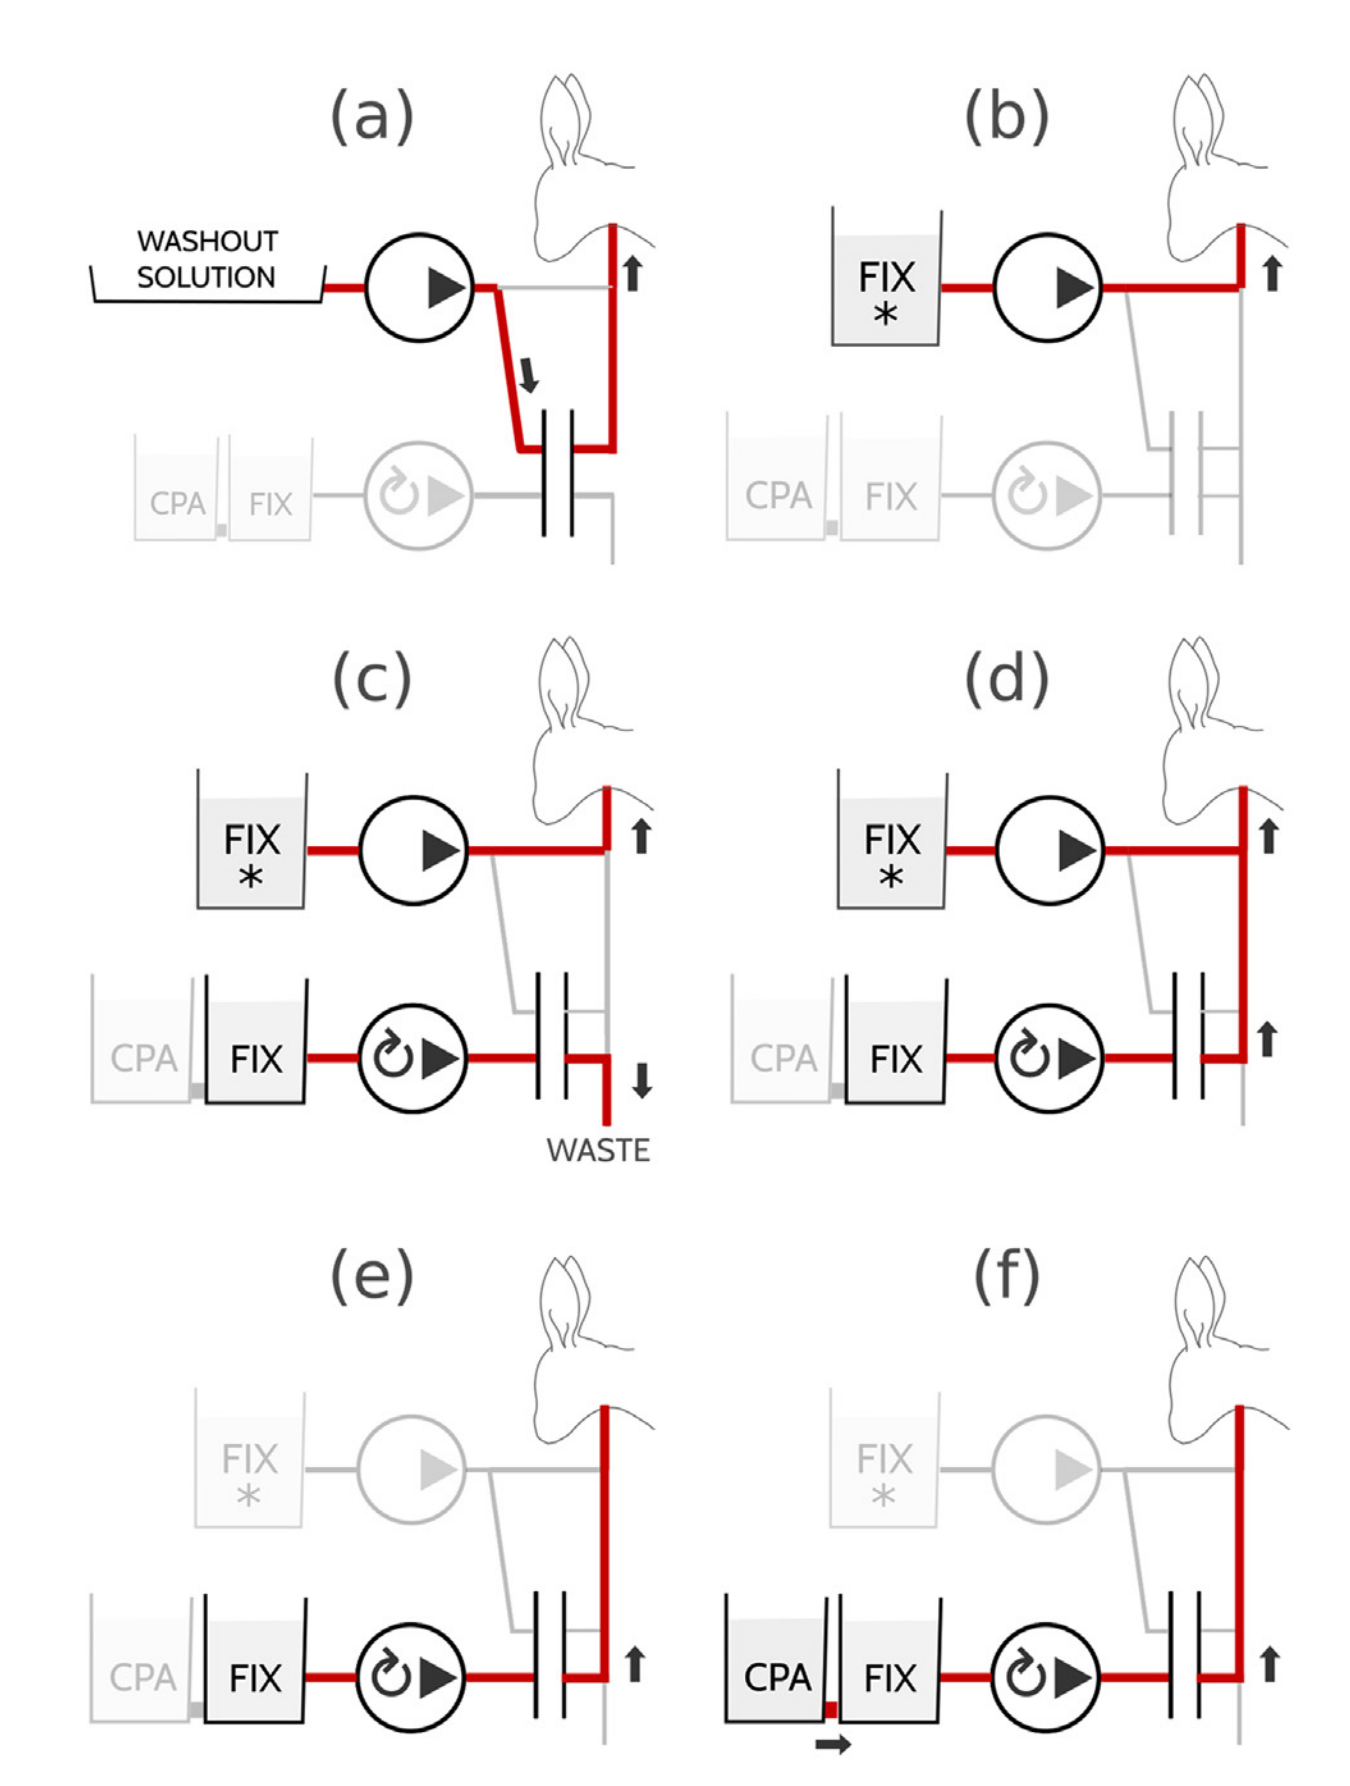
\includegraphics[width=0.50\textwidth]{bunny_perfusion_diagram.png}
\caption{\label{fig:Prefusion_figure}Perfusion Process Diagram \cite{Aldehyde_stabilized_cryopreservation}}
\end{figure}

\subsubsection{Cryoprotectant}
\label{chemical_cryoprotectant}

The brain must be frozen to reduce the effects of chemical and physical processes mentioned earlier in the report. In order to prevent freeze-induced cell damage, a cryoprotectant is required. We require a cryoprotectant that has a low molecular weight and is nontoxic \cite{cyrogenanimalcellcultures}. The cryoprotectant also needs to provide high levels of cell viability post thaw, and must not alter the cells in any way, or cause them to behave differently after exposure to the cryoprotectant \cite{Cryoprotectantsoptions}.

Cryoprotectants can be either intracellular or extracellular agents. The main difference between these classes is that intracellular agents are able to penetrate inside the cells, preventing the formation of ice crystals, which could damage or rupture the cell membrane, whilst extracellular agents improve the osmotic imbalance that occurs during freezing \cite{Cryoprotectantsoptions}. Research shows that extracellular agents cannot stop the formation of ice crystals within the cells, leading to a deterioration in the brain sample's cell quality \cite{CryopreservationFelipedeLaraJanz}.

Ethylene glycol, an intracellular agent, has been successfully used as a cryoprotectant for vitrification due to its low formula weight and high permeation into cells compared with other cryoprotectants, including propylene glycol \cite{ethyleneglycol}. The cryoprotectant solution should be identical to the fixative solution, but also contain 65\% w/v ethylene glycol, as seen in Table \ref{Cryoprotectantsolution}. This is to prevent the diffusion of fixative from the brain cell.

\begin{table}[H]
\centering
\begin{tabular}{|l|l|}
\hline
\textbf{Chemical} & \textbf{Concentration} \\ \hline
 \ce{Na2HPO4}.\ce{2H2O} & 14.65 g/L \\ \hline
\ce{NaH2PO4}.\ce{2H2O} & 2.76 g/L \\ \hline
Glutaraldehyde & 3\% w/v \\ \hline
Ethylene Glycol & 65\% w/v \\ \hline
Sodium Dodecyl Sulfate & 0.01\% w/v \\ \hline
Sodium Azide & 0.1\% w/v \\ \hline


\end{tabular}
\caption{Cryoprotectant solution \cite{Aldehyde_stabilized_cryopreservation}}
\label{Cryoprotectantsolution}
\end{table}


\paragraph{Cryoprotectant Method}

\begin{enumerate}
\item Initialise the gradient generator on the perfusion machine.
\item Linearly increase the concentration of cryoprotectants into the perfusion solution over 6 hours. (Automatic pump should ensure target pressure is maintained despite the increase in viscosity).
\item Prepare 1L of fresh cryoprotectant solution which should be circulated around the brain for 1 hour to ensure uniform fixation.
\end{enumerate}

After the initial fixative perfusion process is completed (with the automatic pump replacing the manual one for perfusion) the cryoprotectants should be introduced. Scaling up from the porcine brain (\SI{180}{\centi\metre\cubed})\footnote{http://mste.illinois.edu/malcz/DATA/BIOLOGY/Animals.html [Accessed 05/03/2016]} the fixation solution volume was found to be 17 times the volume of the brain \cite{Aldehyde_stabilized_cryopreservation}. Therefore $Cryoprotectant$ $Volume = Brain$ $Mass \times 17 = \SI{1900}{\centi\metre\cubed}\cite{cosgrove2007evolving} \times \SI{17}= \SI{32300}{\milli\litre} = \SI{32}{\litre}$ of cryoprotectant solution is required.


\subsection{Vitrification}

	\label{Vitrification}

The cryoprotected human brain should now be stored in a controllable isothermal vapour storage unit maintained at -140\degree C. The brain sample should not be removed from the storage unit for the first 24 hours in order to ensure the sample reaches the target temperature. The equipment to be used should be the 21st Century Medicine, Inc. Controllable Isothermal Vapour Storage (CIVS) device together with a Physitemp MT-23 thermocouple needle probe to record the temperature \cite{Aldehyde_stabilized_cryopreservation}. 

\subsubsection{Warming and removal of CPA}
	\label{Warming}

After vitrification, the subject is removed from the CIVS unit and allowed to warm to room temperature in a fume hood for 2 hours. As before, there are two methods for removing the cryoprotectant from the sample - perfusion or diffusion. It is not possible to process and scan the whole brain in one go due to the limited speed at which images of the brain sample can be captured. Therefore, an initial sectioning of the brain should be taken with the remaining brain refrozen for processing at a later stage. Perfusion cannot be used as sectioning the brain will break up the natural vascular network as well as being a costly and time consuming process.

In order to cut down the size of the brain it should be removed from the skull, as detailed in section \ref{brain_removal}. The brain sample should be embedded in agar containing 65\% w/v ethylene glycol to prevent diffusion and sectioned into $\SI{13}{\centi\meter} \times \SI{9.3}{\centi\meter} \times \SI{0.5}{\milli\meter}$ blocks using a compresstome. One section should be cut into $\SI{3.5}{\milli\meter} \times \SI{2.5}{\milli\meter} \times \SI{0.5}{\milli\meter}$ to be imaged using a custom vibratome. The remaining sections should be refrozen for future use. 

To remove the cryoprotectant from the sectioned sample, the sample should be placed in small vials filled with cryoprotectant solution. The cryoprotectant should be removed by an exponential dilution in 0.1 M cacodylate, halving the concentration of cryoprotectant every 10 minutes \cite{Aldehyde_stabilized_cryopreservation}. After 5 rounds of exponential dilution the samples are ready for the next stage.

\subsection{Post Fixation and Staining}
\label{postfixation}

Due to the lack of interaction and contrast within the cell structures, the sample needs to be stained. Staining increases the interaction between the electron beam with the sample providing sufficient contrast in order to detect synapses. The tissue needs to be stabilised further using post fixation techniques. 

The method of scanning electron microscopes, which will be used for scanning the image, as outlined in section \ref{EMChemRef}, captures the back scattering of electrons which have been emitted from the focused electron beam. Clearly, the greater the interaction between the electron beam and the sample the greater the contrast of the resulting image. This demonstrates why heavy atoms are commonly used to stain SEM imagining samples as their high electron density is felt a lot more by the focused electron beam, resulting in greater backscattering and increased contrast of the final image \cite{knott2008serial}. Another advantage to staining is that the staining elements can form further bonds with the sample cells, resulting in further fixation and maintaining the cells' structural integrity \cite{HeavyMetalsWatson}. Numerous methods for staining and post fixation have been developed over the years including OTO (Osmium Tetroxide-thiocarbohydrazide(TCH)-Osmium), rOTO (reduced Osmium Tetroxide-thiocarbohydrazide(TCH)-Osmium), wbPATCO (whole-brain periodic-acid-thiocarbohydrazide-\ce{OsO4}) and BROPA (brain-wide reduced-osmium staining with pyrogallol-mediated amplification). 

Of the staining methods available, BROPA has been chosen as it provides the greatest contrast, uniformity and preservation. The introduction of formamide in a reduced osmium solution allows highly charged molecules to cross membranes. The formation of nitrogen bubbles is stopped by replacing TCH with pyrogallol. It is also the only method of staining that enables the identification of synaptic contacts within EM imaging \cite{highres_em_staining}.

The other methods were discounted for the following reasons. The OTO method suffers from the formation of nitrogen bubbles \cite{wholemousebrain2012}. This in turn reduces membrane contrast limiting the depth to approximately \SI{1}{\milli\meter} as well as creating non-uniform staining and embedding problems \cite{highres_em_staining}. The reduced osmium in the rOTO method uses more reactive staining chemicals, leading to better membrane staining. This method allows a maximum penetration depth of \SI{100}{\micro\metre} - \SI{200}{\micro\metre} but still suffers from nitrogen bubble formation \cite{OTOvsrOTO}. The wbPATCO process allows for greater preservation than the previously mentioned methods. However, the preservation and contrast of membranes and small subcellular structures is insufficient to identify synapses unambiguously \cite{highres_em_staining}. A summary of the staining techniques can be seen in Table \ref{stainingtechiques}.

\begin{table}[H]
\centering

\begin{tabular}{|c|c|c|c|c|}
\hline
\textbf{Staining} & \textbf{Contrast} & \textbf{Uniformity} & \textbf{Preservation} & \textbf{Total} \\ \hline
OTO & 4 & 2 & 1 & \textbf{7} \\ \hline
rOTO & 4 & 3 & 2 & \textbf{9} \\ \hline
\multicolumn{1}{|l|}{wbPATCO} & 4 & 4 & 3 & \textbf{11} \\ \hline
BROPA & 5 & 4 & 4 & \textbf{13} \\ \hline
\end{tabular}
\caption{Staining Techniques}
\label{stainingtechiques}
\end{table}

\subsubsection{BROPA}

\begin{figure}[H]
\centering
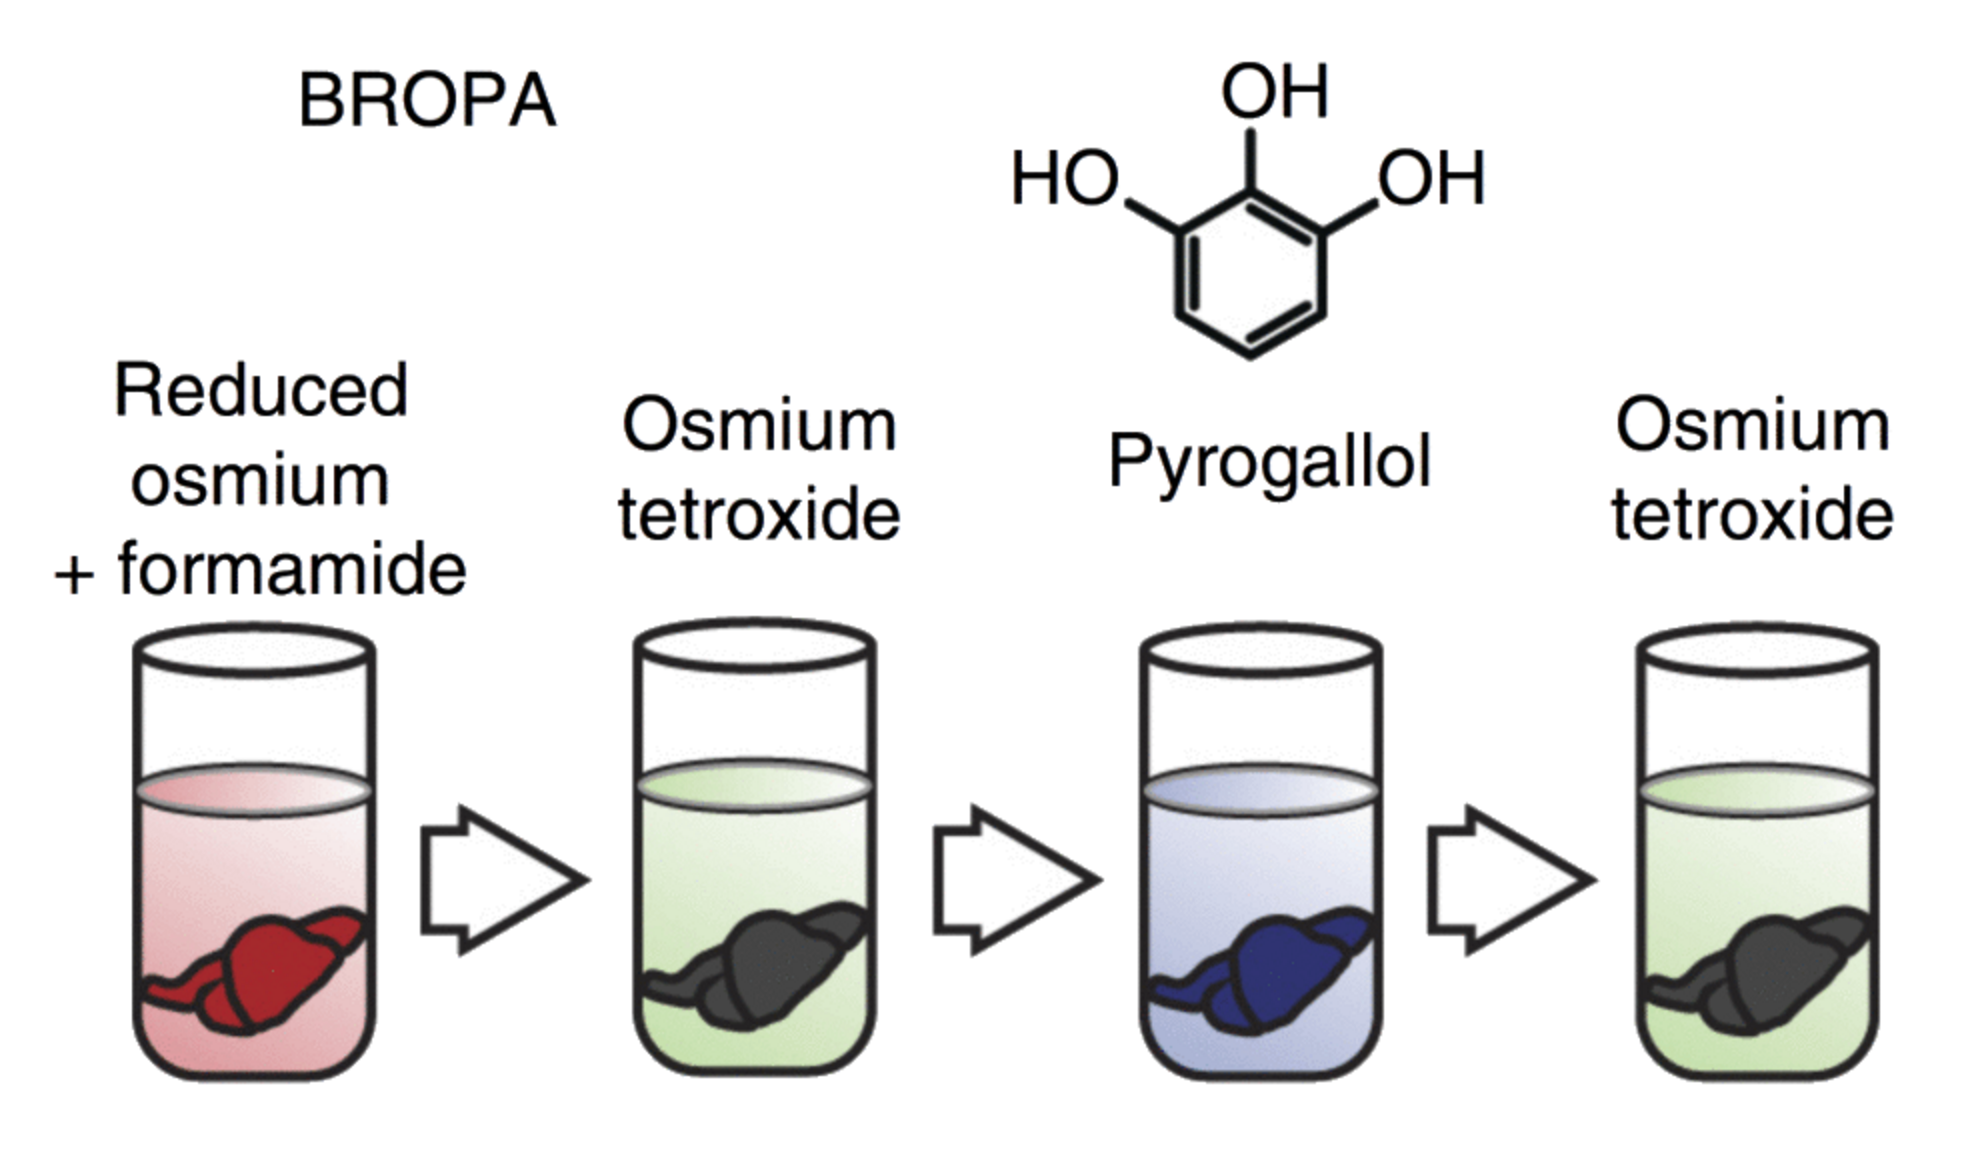
\includegraphics[width=0.50\textwidth]{bropa.png}
\caption{\label{fig:BROPA} BROPA Protocol \cite{wholemousebrain2012}}
\end{figure}	



\paragraph{Reduced Osmium and Formamide}

Reduced osmium and formamide are used in the BROPA protocol due to barrier formation being completely eliminated when crossing cell membranes with staining becoming uniform throughout the sample \cite{highres_em_staining}. Formamide is used as it provides higher membrane contrast and visibility without the loss of most of the cytoplasmic contrast seen with reduced Osmium dioxide \cite{OTOvsrOTO}.


\paragraph{Osmium Tetroxide}
Osmium tetroxide was first used by Palade (1952), whilst trying to identify the function and structure of the cell using an electron microscope. It has since been used throughout history as a fixation and staining agent \cite{OsmiumTetroxidemethod}. The popularity of osmium tetroxide is due to its high atomic mass as well as its bond formations with membranous structures and vesicles. The high atomic mass increases the interaction between the electron beam and the sample making the final image clearer. 

The chemical's ability to form a black reduction compound with membranous structures and vesicles, usually via a double carbon-to-carbon bond, allows for greater membrane and therefore synapse detection \cite{OsmiumTetroxidemethod}. It is also recommended as a post fixative when glutaraldehyde or paraformaldehyde is used as the initial fixative, as the use of other secondary fixatives results in the loss of intracellular structures\footnote{https://www.emsdiasum.com/microscopy/OsmiumTetroxideStainingfTissues.pdf [Accessed 03/04/2016]}.

\paragraph{Pyrogallol}

As mentioned previously, the use of aldehyde fixation results in an osmotic imbalance \cite{Cryoprotectantsoptions}. To correct this imbalance pyrogallol is used which provides extracellular space to improve stain penetration \cite{osmoticimbalance}. Using pyrogallol instead of TCH also stops the formation of nitrogen bubbles \cite{highres_em_staining}.

\subsubsection{BROPA Method \cite{highres_em_staining}}
 	\label{bropa_meth}


\begin{enumerate}
 \item Submerge sample in aqueous solution containing \SI{8.90}{\micro\litre} \ce{OsO4}, \SI{11.30}{\micro\litre} \ce{K4Fe(CN)6}, \SI{12.08}{\micro\litre} sodium cacodylate Buffer (pH 7.4) and \SI{0.10}{\micro\litre} formamide for 60 minutes.
 \item Transfer the sample to an aqueous solution of \SI{8.90}{\micro\litre} \ce{OsO4} and \SI{12.08}{\micro\litre} sodium cacodylate buffer (pH 7.4) for 60 minutes.
 \item Replace the solution with \SI{12.08}{\micro\litre} sodium cacodylate buffer and wait 60 minutes.
 \item Transfer the sample to an unbuffered aqueous solution of \SI{35.31}{\micro\litre} pyrogallol at a pH of 4.1 for 60 minutes.
 \item Replace the pyrogallol solution with \SI{12.08}{\micro\litre} sodium cacodylate buffer for 60 minutes.
 \item Transfer sample to another tube containing an unbuffered aqueous solution of \SI{8.90}{\micro\litre} \ce{OsO4} for 60 minutes.
\end{enumerate}

As the BROPA method was designed for brain-wide staining, the method and amount of chemicals required needs to be scaled accordingly. One paper states that a \SI{1}{\milli\meter} thick block of tissue requires up to 60 minutes for effective diffusion\footnote{http://tissuesampling.weebly.com/processing.html [Accessed 05/03/2016]}, therefore diffusion is assumed to be complete after this 60 minute period. Shawn Mikula and Winfried Denk \cite{highres_em_staining} used 100 times the brain's volume for brain-wide staining. As the sample to be used is smaller (by a factor of 10), the sample size used was 10 times the volume of the human brain. The values of the chemicals in each solution should be calculated to maintain the same concentration as listed in the paper \cite{highres_em_staining}.
 

\subsection{Dehydration}
 	\label{Dehydrate}

To prepare the sample for SEM imaging the brain sample needs to be dried to make it compatible with the vacuum in the electron microscope. If water molecules are present in the sample, it will disrupt the vacuum and result in a poorer image\footnote{http://www.leica-microsystems.com/science-lab/brief-introduction-to-critical-point-drying/ [Accessed 03/04/2016]}. The advantages and disadvantages of potential dehydration methods are outlined below. 

\subsubsection{Exposure}

Early dehydration methods used direct exposure with dry air due to its ease and cost effectiveness. However, as water molecules were removed from the sample they were not replaced resulting in a significant loss in sample mass. The removal of water led to deformations of the sample tissue and therefore poor synapse identification. 

\subsubsection{Freeze Drying}

Freeze-drying is an alternative process, commonly used in the food industry. The process works by freezing the material and then reducing the surrounding pressure to allow the frozen water in the material to sublimate directly from a solid to a gas phase. However, when a glutaraldehyde fixed sample was subjected to the freeze drying process it was found to shrink to 51\% of its original volume \cite{freezedryingvscriticalpoint}. Again this will result in deformations of the sample tissue and poor synapse identification. 

\subsubsection{Critical Point Drying}

Another potential dehydration method is critical point drying (CPD). This method uses the critical point of water where solid, liquid and vapour can exist simultaneously. At this triple point, the physical characteristics of liquids and gases are not distinguishable. Therefore, the water within the cell can be converted from liquid to vapour and then be displaced from the cell in the vapour state, thus avoiding any damage caused by surface tension. To combat the issue of shrinkage and mass loss, water is commonly replaced with liquid carbon dioxide, whose critical point lies at 31\degree C and 74 bar which is technically easier to maintain, compared with the critical point of water\footnote{http://www.leica-microsystems.com/science-lab/brief-introduction-to-critical-point-drying/ [Accessed 03/04/2016]}. However, as \ce{CO2} is not miscible with water, the process requires an exchange fluid such as ethanol in order to replace the water. Reports show that the sample still shrunk by up to 38\% during dehydration. Whilst an improvement on previous methods, this complex exchange process led to sample deformation and tissue damage \cite{freezedryingvscriticalpoint}.

\subsubsection{Solvent Dehydration}

The solvent dehydration process is accomplished by passing the tissue through a series of increasing alcohol concentrations. This method works as the solvents used are hydroscopic, having the ability to attach and hold water molecules from the surrounding environment. The dehydration protocol involves the slow substitution of the water in the tissue with an organic solvent \cite{dehydrationmethod}. The concentration gradient of the solvent used should increase regularly and linearly in order to avoid excessive osmotic pressure, which would result in membrane distortion and damage to the cells.

The advantage of using solvent dehydration compared with critical point drying (CPD), the next best alternative, is that despite the shrinkage in the sample being similar, when processed using CPD the sample suffers from severe cracking of cell processes and microcracks across cell membrane surfaces \cite{JEMT1070300508}. This could be due to the complex exchange process.

\subsubsection{Solvent Dehydration Method}

There are a variety of different solvents that have been used in the dehydration method including toluene, dichloromethane, acetonitrile, methanol and ethanol; however research shows that ethanol is the most effective at removing water from a sample \cite{jo101589}.

\begin{enumerate} 
 \item Rinse sectioned sample for 20 minutes in double distilled water.
 \item Transfer the sections of tissue sequentially to 30\%, 50\%, 70\%, 80\%, 90\%, 95\%, and 100\% ethanol for two hours each.
 \item Place the sections in a second 100\% ethanol solution for 1 hour to ensure that all water is removed.
\end{enumerate}

Note that only absolute ethanol can be used to ensure maximum water removal from the sample \cite{dehydrationmethod}. The volume of each ethanol solution should be 10 times the volume of the sample to ensure complete dehydration. Therefore, $Ethanol$ $Volume = Tissue$ $Volume \times 10 = \SI{3.5}{\milli\metre} \times \SI{2.5}{\milli\metre} \times \SI{0.5}{\milli\metre} \times 10= \SI{0.04375}{\milli\litre\cubed}$ of ethanol is required.


\subsection{Embedding}
\label{Embed}
The final stage in preparing the sample for imaging is resin embedding. This stage is required to harden the sample further to ensure it maintains its structural integrity; with the resin providing mechanical support during final sectioning and subsequent imaging. The embedding should improve the uniformity during sectioning as well as reducing cell loss. 

There are two major types of resin embedding commonly used - epoxy and acrylic resins. Epoxy resins are recognised for their uniform hardening and strong sectioning properties. They also change very little in volume when used as a resin. Acrylic resins, due to their low viscosity, even at low temperatures are miscible in water. They also have a low toxicity reducing damage to the brain sample. Consequently, they are the preferred resin of choice for EM imaging, despite the fact that the preservation itself may not be as good as an epoxy resin \cite{embeddinghistory}. Additionally, acrylic resin can be used in combination with numerous other processes making it such a popular choice in tissue preparation processes \cite{resinforem}.

Due to their popularity numerous commercial acrylic resins have been produced. The three most popular ones are LR White, Lowicryl and Unicryl \cite{embeddinghistory}. Numerous studies have been completed to determine the best acrylic resins. One study shows that immunohistochemical tissue embedded in Unicryl resulted in significantly stronger labelling than an identical tissue embedded in Lowicryl K4M \cite{UnicrylversusLowicryl}. Another study showed that Unicryl was again preferred to LR White as it provided better preservation and improved immunodetection efficiency \cite{LRWhitevsUnicryl}. Based on these papers Unicryl acrylic resin should be used for embedding the sample.

\subsubsection{Unicryl}

Using Unicryl should provide excellent structural preservation of tissue without chemically interacting or crosslinking with it. This ensures that the sample remains chemically unaltered whilst providing the rigidity required in the final sectioning and imaging of the sample. Unicryl is able to achieve this as its components have a similar molecular weight to the tissue sample ensuring even penetration. All acrylic resins are hydrophilic, exhibit low background staining and minimise the denaturing of proteins. In addition, when being sectioned for imaging, the Unicryl resin ensures that sections are cleaved ahead of the knife edge resulting in greater exposure of the tissue components at the surface \cite{UNICRYL}.

The resin needs to be polymerized. This can be achieved by two methods: by either heat or UV irradiation. As the sample will remain unaffected by heat, it should be polymerized at 60\degree C for two days to ensure quick and efficient polymerization, preventing the sample from becoming brittle. Equally, it has been proven to produce clear results when used with the dehydration agent ethanol \cite{UNICRYL}.

\subsubsection{Embedding Method \cite{UNICRYL}}

\begin{enumerate} 
\item Infiltrate with 100\% resin for 2 hours while agitating gently on a shaker or rotating wheel.
\item Infiltrate with fresh resin for 10 hours to allow full penetration.
\item Heat sample at 60\degree C for 48 hours.
\item Once complete the tissue sections should be sent to the ATUM (Automated Tape-collecting Ultra-Microtome) for final sectioning and imaging.
\end{enumerate}

The volume of embedding solution required is 10 times the tissue volume. Therefore, the total amount of Unicryl solution required is obtained from the following formula: $Embedding$ $Volume = Tissue$ $Volume \times 10 = \SI{3.5}{\milli\metre} \times \SI{2.5}{\milli\metre} \times \SI{0.5}{\milli\metre} \times 10= \SI{0.04375}{\milli\litre\cubed}$.

\subsection{Automation of Chemical Preparation}
The overriding objective for chemical preparation is to develop a reliable, repeatable method for preparing the brain for final sectioning and imaging. Achieving this as efficiently and cost effectively as possible requires process automation. Automation should result in greater uniformity within samples, due to the greater precision over chemicals. The probability of human error should be significantly decreased. Data loss should be minimised and the time and cost of the process reduced.

There are numerous automated tissue processors available. The LYNX II Automated Tissue Processor for Histology and Microscopy\footnote{https://www.emsdiasum.com/microscopy/products/equipment/tissue\_processor.aspx [Accessed 05/03/2016]} allows for 24 samples to be processed simultaneously, whilst the EMS Poly III Evaporation-Controlled Automated Embedding and Polymerization is able to embed 52 samples simultaneously\footnote{https://www.emsdiasum.com/microscopy/products/equipment/polymerization.aspx [Accessed 05/03/2016]}

As the initial fixation and adding of the cryoprotectant only needs to be completed once for the whole brain, there is limited benefit to automating these activities. When determining the amount of time it takes to complete the chemical preparation process the following activities have been considered: the time required for post fixation, staining, dehydration and embedding of the section brain sample. The table \ref{chemprocesstime} below shows a breakdown of the time required for each stage.

\begin{table}[h]
	\centering
	\begin{tabular}{|l|l|}
		\hline
		\textbf{Process} & \textbf{Time} \\ \hline
		Post Fixation \& Staining - BROPA &  \multicolumn{1}{r|}{6 hours} \\ \hline
		Dehydration - Ethanol Dehydration Method &\multicolumn{1}{r|}{16 hours} \\ \hline
		Embedding - Unicryl & \multicolumn{1}{r|}{60 hours} \\ \hline
		\textbf{Total} & \multicolumn{1}{r|}{\textbf{82 Hours}} \\ \hline
	\end{tabular}
	\caption{Breakdown of time required for Chemical processes}
	\label{chemprocesstime}
\end{table}

Number of sections to process is $\dfrac{Volume\;  of\;  Brain}{Volume\; of\;  section}$ = $\dfrac{\SI{1900}{\centi\meter\cubed} }{\SI{3.5}{\milli\meter} \times \SI{2.5}{\milli\meter} \times \SI{0.5}{\milli\meter}} = 434286$ sections. 

If only one LYNX II Automated Tissue Processor for Microscopy is used, which can process 24 sections in one go, it will take $\dfrac{434286}{24}\times 82$ $hours = 1483808$ $hours = 169.4$ $years$ to complete the chemical preparation. 

If 170 Automated Tissue Processors are used it will take just under a year to complete the chemical preparation. 


\subsection{Conclusion}

This section describes the key stages of the chemical preparation process for preparing the brain for final sectioning and imaging, in order to best identify synapses within the brain. The challenges of protecting the state of the brain after death are described. The importance of the fixation process is highlighted and how perfusion can be used to deliver the fixative to all areas of the brain. The report describes the benefits of using a cryoprotectant to protect the sample from freeze-induced cell damage, as well as providing a way of refreezing the sample. This ensures that its structure does not deteriorate, whilst processing smaller parts of the brain for imaging. By dividing the brain into smaller sections post fixation, it has been shown that an automated approach for post fixation, dehydration and resin embedding can be applied. Through the introduction of automation, it is possible to be more precise with the sample, generating more uniform results, as well as being able to take advantage of economies of scale. By using an automated tissue processor, the cycle time for completing the chemical preparation process could be reduced to less than a year. 

\newpage

\clearpage

\pagestyle{judah}


	\section{Brain Removal}
	\label{brain_removal}
	Initially the brain must be removed from the head of the participant after it has been thawed. The protocol for removing a human brain has been well documented in autopsy training manuals, such as that provided by Brown University.
	
The method from the from \cite{autopsy} is reproduced below:
	\begin{enumerate}
		\item An incision is made coronally from the mastoid process to the contralateral mastoid process. 
		\item The skin and muscle of the scalp can then be reflected to expose the skullcap.
		\item A cut which extends horizontally from the centre of the forehead to the base of the mastoid process on both sides with a bone saw. A notch is normally cut at the centre of the forehead to allow for more stable repositioning of the skullcap.
		\item Another cut is made from the posterior superior surface of the skull such that the angle from this cut to the first cut is more than 90\textdegree.
		\item The brain is removed by drawing back the frontal lobes.
		\item Optic nerves and carotid arteries are cut together with the pituitary stalk.
		\item The temporal lobes are lifted and the tentorium is cut with scissors or a scalpel blade and the cervical spine is severed.
		\item The brain can then proceed to the next phase of our sectioning pipeline.
	\end{enumerate}
	
	It is crucial that this process is conducted with as much care as possible by a highly skilled pathologist so as to minimise the physical damage which is done to the structure of the brain.
	
	\newpage
	\section{Sectioning}
	\label{sectioning}
	
	We will begin this section of the process design by making some estimates of the dimensions of the human brain. The dimensions of a human brain are approximately \SI{130}{\milli\metre} x \SI{170}{\milli\metre} x \SI{93}{\milli\metre}\cite{hassanali2007comparative}. For the purposes of this design the brain will be modelled as a cuboid with these dimensions. This clearly will result in an overestimation of the volume of the brain but should give a good idea for the upper limits of cutting times.
	
	In order to ensure that we are able to obtain the necessary information from the client's brain our scanning electron microscopes\footnote{Reasons for use of scanning electron microscopy (SEM) detailed in Section \ref{EMChemRef}} must be provided with slices of brain tissue in the order of tens of nanometres thick. This ensures that the loss of a single section is unlikely to result in significant loss of data. It is not possible to simply slice a whole brain into ultra thin slices in one step and so in this section various methods for sectioning the brain on different scales will be discussed and a pipeline for producing these ultra-thin slices will be designed.
	
	
	\subsection{Final Sectioning}
	It makes sense to begin the design considerations with the final sectioning method. This is because the most rigid constraints on section dimensions will be dictated by which process is chosen for this step.
	\subsubsection{Focus Ion Beam Milling (FIB)}
	\label{sectioning_smallest_FIB}
	Focused ion beam milling has, until relatively recently, been primarily used in the semiconductor industry. Recently it has been used for scanning electron microscopy and has been used with great success in neural imaging\cite{knott2008serial}\cite{lich2016automated}. This method uses a focused beam of gallium ions parallel to the surface of the tissue sample to mill away the ultra-thin sections. These sections can be less than \SI{3}{\nano\metre} thick\footnote{http://www.zeiss.com/microscopy/en\_de/products/fib-sem-instruments/crossbeam.html\#download [Accessed 03/03/2016]} which would allow for isotropic resolution. This would provide a significant advantage for automatic segmentation algorithms discussed in Section \ref{segmentation} and would ensure minimal data loss in the event of lost sections. Given that the average diameter of synaptic vesicles, which are the smallest structures which we intend to image, are approximately \SI{50}{\nano\metre}\cite{purves2001release} this resolution would allow us an error of losing up to four consecutive sections assuming a milling resolution of \SI{10}{\nano\metre}.
	
	\begin{figure}
		\centering
		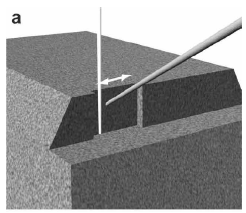
\includegraphics[width = 0.35\textwidth]{FIB_milling}
		\caption{Three-dimensional drawing of the resin block showing the arrangement of the gallium ion beam (white) that scans parallel to the block (indicated by double-headed arrow) and mills away a layer of resin, creating an imaging face \cite{knott2008serial}.}
		\label{FIB_milling}
	\end{figure}
	
	The process of milling a resin embedded sample using FIB begins by mounting the resin block on the milling device (which usually also performs the SEM imaging) and coating it with a thin layer of platinum. The gallium ions mill the sample by colliding with and ejecting molecules from the block face as well as reacting with a precursor gas (methylcyclopentadienyl (trimethyl) platinum (IV)). This gas is injected to continually deposit a thin layer of platinum on the sample's surface. This layer of platinum, as well as removing any surface charge which would affect the quality of the electron micrographs, reduces milling artefacts and ensures that the milling remains parallel to the surface\cite{heymann2006site}. 
	
	It is also important to appreciate the limitations of FIB milling. The first limitation to address is the extremely small field of view and slow milling speed. To understand how limiting these problems are some simple calculations for the total time to mill a human brain can be made. According to Knott et al. \cite{knott2008serial} the time taken to mill \SI{900}{\micro\metre\squared} is \SI{75}{\second} using an acceleration voltage of \SI{30}{\kilo\electronvolt} and a current of \SI{1000}{\pico\ampere} with a milling depth of \SI{20}{\nano\metre}. If we take the upper expected volume of a human brain as \SI{1900}{\centi\metre\squared}\cite{cosgrove2007evolving} then we can calculate the total milling time as follows:
	
	\begin{align}
	Number\ of\ Mills\ Required &= \frac{Volume\ of\ Brain}{Milling\ Depth \times Milling\ Area} \nonumber \\
	&= \frac{1900\times10^{-6}}{20\times10^{-9} \times 900\times10^{-12}} = 1.06\times10^{14} \nonumber \\
	Total\ Milling\ Time &= Milling\ Time \times Number\ of\ Mills\ Required \nonumber \\
	&= 75 \times 1.061\times10^{14} = 7.92\times10^{15} seconds \nonumber \\
	&= 251\ machine\ million\ years
	\end{align}
	
	Clearly we cannot use FIB milling as a method for sectioning and imaging an entire human brain as the process takes too long. It would take even longer if we milled at a depth of \SI{10}{\nano\meter}
	
	\subsubsection{Serial Block Faced Scanning Electron Microscopy (SBSEM)}
	\label{sectioning_smallest_SBSEM}
	\begin{figure}[!h]
		\centering
		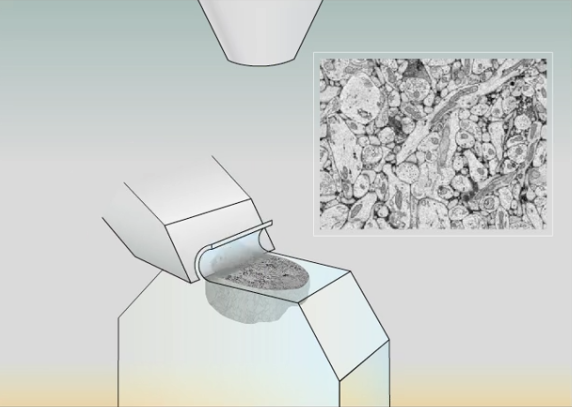
\includegraphics[width = 0.35\textwidth]{SBSEM}
		\caption[stuff]{Image showing the mechanism of SBSEM\footnotemark}
		\label{SBSEM_illustration}
	\end{figure}
	\footnotetext{Illustration courtesy of Julia Kuhl, www.somedonkey.com.}
	A method which is similar to FIB is serial block face imaging using an ultramicrotome. Figure \ref{SBSEM_illustration} depicts the operation of a typical SBSEM. The blade sweeps across the sample removing a thin layer, returning to its original position as the sample advances one section thickness vertically. This allows for alignment to remain constant and for each image to remain in focus. This offers a number of advantages over FIB as well as a number of shortcomings. Like FIB milling, serial block face imaging using an ultramicrotome offers the advantage that very little aligning needs to be conducted after imaging due to the nature of the sample advance mechanism. SBSEM also shares the advantage of being highly automatable with excellent reliability. Section thickness is commonly about \SI{25}{\nano\metre} which allows for a single section to be lost without significant data loss. Although this is not as robust as FIB milling it is extremely unlikely that two consecutive sections will be lost. The field of view which can be imaged is also substantially larger\cite{denk2004serial}.
	
	The biggest disadvantage of SBSEM when compared to FIB milling is the presence of cutting defects, these include chattering, compression and knife marks \cite{hashimoto20163d}. The chattering can be reduced by using an oscillating blade \cite{studer2000minimal} and knife marks can be reduced by using a highly polished diamond knife. Compression artefacts can, however, only be minimised by either reducing cutting speed or using a sharper knife. Although some blades have a cutting edge as small as \SI{4}{\nano\metre} wide it is unlikely that ones will soon become available.
	
	The diamond knives used in ultramicrotomes have traditionally been limited in length to about \SI{4}{\milli\meter} due to the need for the knife to be formed from a single crystal. This has limited the area which can be sectioned to a size in the order of \SI{0.5}{\milli\metre} x \SI{0.5}{\milli\metre} x \SI{25}{\nano\metre}\cite{briggman2011wiring}. Diatome, a Swiss diamond knife manufacturing company, has, however been developing a \SI{1}{\centi\metre} diamond knife for use by Dr Winfried Denk in SBSEM since 2013. There have been significant difficulties in producing this knife. However, a prototype has now been delivered to Dr. Denk although testing has not yet been conducted. Diatome offers an \SI{8}{\milli\meter} knife which is suitable for SBSEM\cite{diatome_gnaegi}. This would dramatically increase the cross sectional area of each section over that produced using a \SI{4}{\milli\meter}. long knife.
	
	Using a typical cutting speed of an SBSEM as \SI{0.5}{\milli\meter\per\second} \footnote{http://www.gatan.com/products/sem-imaging-spectroscopy/3view-system [Accessed 04/04/2016]}, and the total section volume to be increased by using an \SI{8}{\milli\metre} knife to \SI{3}{\milli\metre} x \SI{3}{\milli\metre} x \SI{25}{\nano\metre}, some estimates for total cutting time can be made to test SBSEM's feasibility. An upper estimate of the volume of a human brain is again taken to be \SI{1900}{\centi\metre\cubed}\cite{cosgrove2007evolving} .
	
	\begin{align}
	Number\ of\ Cuts\ Required &= \frac{Volume\ of\ Brain}{Section\ Volume} \nonumber \\
	&= \frac{1900\times10^{-6}}{25\times10^{-9} \times 9\times10^{-6}} = 8.44\times10^{9} \nonumber \\
	Cut\ Time &= \frac{Cut\ Length}{Cutting\ Speed} = \frac{3}{0.5} = 6\ seconds \nonumber \\
	Total\ Cutting\ Time &= Cut\ Time \times Number\ of\ Cuts\ Required \nonumber \\
	&= 6 \times 8.44\times10^{9} = 5.07\times10^{10} seconds \nonumber \\
	&= 1608\ machine\ years
	\end{align}
	
	This is a much more reasonable period of time. It should be noted, however, that this excludes any imaging time (discussed in detail in Section \ref{EMChemRef}). This time could, obviously, be further reduced by using multiple SBSEM devices.
	\subsubsection{Laser Microtomy}
	\label{sectioning_smaller_laser}
	
	\begin{figure}[h]
		\centering
		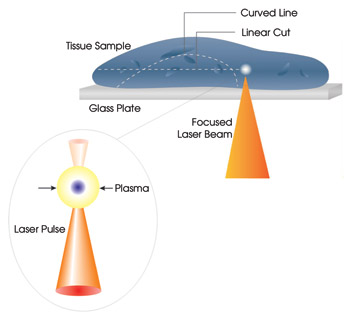
\includegraphics[width=0.4\textwidth]{laser_microtome}
		\caption{Working principle of a laser microtome\cite{lubatschowski2007laser}.}
		\label{laser_microtome}
	\end{figure}
	
	Laser microtomes are a relatively new innovation with the first commercially available device appearing in 2007. Such devices function by focusing a near-infrared laser, normally with a wavelength in the order of \SI{1000}{\nano\meter} onto the specimen. Due to the extreme intensities up to \SI{1}{\tera\watt\per\centi\meter\squared} multi photon absorption causes ionization of the tissue. This is called optical breakdown and results in the formation of plasma. It is this rapid expansion which is responsible for the cut\cite{lubatschowski2007laser}. The advantages of laser microtomy are 1) that as the process is contact free therefore, there is no requirement for freezing, resin or paraffin embedding and 2) typical cutting area of \SI{14}{\milli\meter} x \SI{14}{\milli\meter} is relatively large. The third advantage is excellent ultrastructure preservation is also maintained due to the contact free nature of the process. Unfortunately, commercially available laser microtomes have a minimum cutting thickness of \SI{5}{\micro\metre} which is roughly two orders of magnitude too thick for our requirements.
	
	Near-infrared lasers have also been used for laser-capture microdissection (LCM) and more recently nanodissection of human chromosomes. This method has been demonstrated to be capable of producing cuts with a width of \SI{200}{\nano\meter}\cite{konig2001nanodissection}. This is significantly smaller than the diffraction limited spot size and is only possible because only the centre of this spot delivers sufficient photon density to cause optical breakdown. Although this offers promise to advancements in laser microtomy this would still result in unacceptable tissue loss between sections and so we must conclude that laser microtomy is unsuitable for our purposes.
	\subsubsection{Automated Tape-Collecting System Ultra-Microtome (ATUM)}
	\label{sectioning_smaller_ATUM}
	
	ATUM uses a conventional diamond knife water boat to slice ultrathin sections from a resin embedded sample mounted in a chuck. The sample is passed over the knife blade removing a single section, this section is floated in the water boat before being automatically collected onto a partially submerged conveyor belt made of sturdy plastic tape. The ultramicrotome chuck can then be advanced and another section removed. The water level in the knife boat is controlled automatically with a digital syringe pump and a video feedback system. The only human interaction which is required is resetting the ultramicrotome's advance system approximately every \SI{100}{\micro\meter} and replacing the tissue blocks once the entire block has been sectioned\cite{hayworth2014atum}\cite{schalek2011atum}. This system is shown in Figure \ref{ATUM}. This long tape containing thousands of ultrathin sections can then be cut and mounted to silicon wafers for imaging in a scanning electron microscope.
	
	\begin{figure}[h]
		\centering
		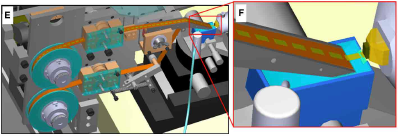
\includegraphics[width=\textwidth]{ATUM}
		\caption{CAD rendering of ATUM showing path collected sections take from the knife boat to the final take-up reel.\cite{hayworth2014atum}}
		\label{ATUM}
	\end{figure}
	
	This method is capable of reliably producing a section thickness of \SI{30}{\nano\meter} at a rate of between 1,000-10,000 sections over a \SI{24}{\hour} period, depending of section area, with minimal human interaction\cite{hayworth2014atum}. This relatively fast acquisition rate coupled with excellent reliability (>10,000 consecutive sections have been collected without missing a cut) It has also been shown that at this section thickness and loss rate that manual segmentation is nearly flawless \cite{kasthuri2015saturated}.
	
	ATUM also offers two additional crucial advantages over the other sectioning methods discussed previously. The first of these is that the sections can be stored once they have been sectioned. This allows for images which were captured incorrectly (i.e. poor contrast) to be noticed and recaptured, offering security. Due to the fact that it is impractical to store all of the images which are acquired, as discussed in Section \ref{data_storage}, if it is discovered that we have overlooked an important structural feature which is needed for the reconstruction of the human brain it will be possible, although extremely costly, to reimage the brain to extract the needed information. This is not a feature of block face methods since sections are  immediately destroyed in FIB or discarded in SBSEM and laser microtomy.
	
	The second important advantage of an ATUM based approach is that whereas with block face approaches there is an inherent limitation of one electron microscope per tissue block, with ATUM it is possible to send the sections from a single ATUM to many microscopes. This separation of cutting and imaging builds in flexibility and allows the number of segmenting and/or imaging machines used to dictate the total rate of image acquisition. Imaging takes much longer than sectioning so separating the two, as in this system, but not in use of block face methodologies means the bottleneck can be avoided. On the other hand, the flexibility provides the possibility of sacrificing speed in the interests of economy as necessary.
	
	It is useful to consider the number of silicon wafers which would be required to image the entire human brain at once. This can be done by estimating the volume of brain which will fit onto each wafer as follows: $Wafer\ volume = Section\ volume \times 170$, where 170 is he approximate number of sections per wafer. The volume of each section can be estimated to be $3.5mm \times 2.5mm \times 30 nm = 2.63\times10^{-13}\ m^3$. This results in a $volume\ per\ wafer = 4.46\times10^{-11}\ m^3$ Therefore:
	
	\begin{equation}
	Number\ of\ Wafers = \frac{Volume\ of\ Brain}{Volume\ per\ Wafer} = \frac{1900\times10^{-6}}{4.46\times10^{-11}} = 4.26\times10^{7}\ Wafers
	\end{equation}
	
	From this number it can be seen that it is impractical to attempt to acquire and store this number of wafers. Instead it makes much more sense to reuse the same wafers for more than one set of samples. This can be done by removing the samples from the wafer after scanning and storing them in an organised fashion separately. The wafers can then be reused. This will limit both the purchase cost of the wafers and the recurring storage cost.
	
	\begin{figure}[h]
		\centering
		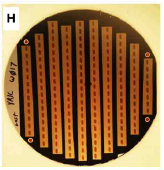
\includegraphics[width=0.35\textwidth]{silicon_wafer}
		\caption{One \SI{100}{\milli\meter} silicon wafer with 162 ultrathin sections. \cite{hayworth2014atum}}
		\label{silicon_wafer}
	\end{figure}
	
	Once again, estimates for the total cutting time involved should be made. This is done by assuming that 10,000 sections with dimensions of \SI{3.5}{\milli\meter} x \SI{2.5}{\milli\meter} x \SI{30}{\nano\meter} can be obtained.
	
\begin{align}
Total\ Number\ of\ Sections &= \frac{Volume\ of\ Brain}{Section\ Volume} \nonumber \\
&= \frac{1900\times10^{-6}}{2.5\times10^{-3} \times 3.5\times10^{-3} \times 30\times10^{-9}} = 7.24\times10^{9} \nonumber \\
Total\ Number\ of\ Days &= \frac{Total\ Number\ of\ Sections}{Sections\ per\ Day} = \frac{7.24\times10^9}{10000} = 7.24\times10^{5}\ days \nonumber \\
&= 1984\ machine\ years \nonumber \\
\end{align}

This is a much more reasonable period of time. It should be noted, however, that this excludes any imaging time (discussed in detail in Section \ref{recording_EM}). This time could, obviously, be further reduced by using multiple SBSEM devices.
\newpage

	\subsubsection{NanoKnife}
		\pagestyle{john}
	
	An alternative experimental cutting technique is the use of a carbon nanotube based nanoknife, designed to work with frozen samples - it boasts the same benefits as the cryostat in section 4.2.4. Using a standard diamond or glass knife can lead to compressive stresses  as the sample bends away sharply from the block face. This can cause cracking once laid flat which results in irreversible tissue damage that will show in the imaging process, and ultimately result in less synapses being detected by our machine learning algorithm\cite{singh2009fabrication}. When multiple layers of graphite are superimposed and rolled in on themselves they form a Multi-Walled Carbon Nanotube (MWCNT), these have up to 20 times the strength of steel and the same thermal conductivity of diamond\footnote{http://www.cefic.org/Documents/Other/BenefitsofCarbonNanotubes.pdf [Accessed 10/03/2016]}. We can use this high tensile strength to our advantage much in the same way as a cheese wire, replacing the conventional diamond knife by welding a MWCNT between tungsten needles. Unfortunately, for now at least, this is where the benefits end. The nanowire has a diameter of ~60 nm, which compared to the cutting edge of 4 nm for the diamond knife is very large. Whilst the tensile strength is extremely good, the welding points tend to show weakness. Given a maximum deflection $\delta_{max}$ of 290  nm and force constant K of 2.8 nm$^{-1}$ we can use the familiar equation:
	\begin{align}
	F_{max} = K\delta_{max}\nonumber 
	\end{align}
	
	This gives a max force of 812nN\cite{singh2009fabrication} before sheer stresses on the welds become too great. To achieve a force below this limit would require incredibly slow speeds and may not even be possible, especially considering frozen tissue. Therefore, despite the idea of using carbon nanotubes being appealing in practice, there simply isn't enough research into their use as cutting devices. Future developments may lead to much longer nanotubes resulting in better attachment and a new method that can be used relatively cheaply. Due to no evidence of current use, and the lack of evidence it could be used in its current state, we will not include this method in further discussion.
	\newpage
	\subsubsection{Discussion}
	\begin{table}[h]
		\centering
		\caption{Comparison of viable final sectioning techniques.}
		\label{finalsectioning_table}
		\begin{tabular}{|l|l|l|l|}
			\hline
			\textbf{Method}            & \textbf{FIB} & \textbf{SBSEM} & \textbf{ATUM} \\ \hline
			Minimum Z-Resolution (section thickness) ( nm)  & 3            & 25             & 30            \\ \hline
			Total Time (machine years) & 251 million  & 1608           & 1984          \\ \hline
			Separation of cutting and imaging                 & No           & No             & Yes           \\ \hline
			Sample Preservation        & No           & No             & Yes           \\ \hline
			Machine Cost               & High         & Low            & Low           \\ \hline
		\end{tabular}
	\end{table}
	
	From Table \ref{finalsectioning_table} it is clear to see that each of the three viable techniques has its own advantages and disadvantages. FIB is capable of giving isotropic resolution but is so slow that it would be impossible to acquire enough machines to section an entire human brain in any practical period of time. For this reason, FIB milling can be ruled out. This leaves SBSEM and ATUM as possible options. Both methods allow for similar z-resolutions and have comparable imaging times. The design choice, therefore, comes down to the benefit of being able to separate cutting and imaging, thus avoiding the bottleneck created by imaging and the advantages of storing the tissue samples after they have been imaged. It is extremely important to us that our process does result in the reconstruction of our customer's brain. Because of this the ability to store the tissue samples after they are imaged is an extremely important advantage of the ATUM method. Our process is currently exclusively aimed at extracting a neural map of our customer's brain. As discussed in Section \ref{intro} there are suggestions in the neuroscience community that this may not, in fact, be enough information to reconstruct the brain. It is, therefore, crucial that it is possible to revisit the brain in light of new discoveries and extract additional information if needed. For this reason, ATUM has been chosen as our final sectioning technique.
	\pagestyle{judah}
	\subsection{Initial Sectioning}
	\label{sectioning_small}
	
	Now that ATUM has been selected for the final sectioning of the tissue samples it must be determined how the brain will be reduced to \SI{3.5}{\milli\meter} x \SI{2.5}{\milli\meter} x \SI{30}{\nano\meter} blocks. It is also important that we are able to deliver these blocks to post-fixation chemical processing pipeline (Section \ref{postfixation}) as quickly as possible so as to minimise the period of time that the samples are fixed by only glutaraldehyde. It is also, however, even more important to ensure that ultrastructure damage is limited between sections.
	
	The first step to producing these sections is to slice the brain coronally into sheets. To limit volume of tissue and so the quantity of data being processed at any one time these sheets will be of the smallest final dimension of the tissue blocks for ATUM (\SI{0.5}{\milli\meter}). There are a number of common ways for biological samples to be sectioned on this scale, most of which will be discussed in this section.
	
	\subsubsection{Tissue Chopper}
	\label{sectioning_small_tissuechopper}
	
	Tissue choppers are the simplest device used in preparation of brain samples. These devices move a sample under a knife blade (commonly a conventional razor blade) and drop the blade onto the sample to make a cut, like a guillotine. This technique is considered to produce inferior results to other methods discussed here such as the vibratome due to the increased pressure on the sample \cite{walz2002patch} although is faster and simpler. The problem of pressure will be even more detrimental in this use case due to the sample being so large.
	
	\subsubsection{Vibratome}
	\label{sectioning_small_vibratome}
	
	Vibratomes function in a similar way to conventional microtomes with the difference being that a vibratome's blade oscillates at high frequency. This reduces cutting artefacts which are the result of pressure on the sample by the knife. These maintain good ultrastructure quality, however, high quality commercially available vibratomes such as the Leica VT1200 S\footnote{http://www.leicabiosystems.com/histology-equipment/sliding-and-vibrating-blade-microtomes/vibrating-blade-microtome/details/product/leica-vt1200-s/ [Accessed 08/04/16]} are unable to accommodate and slice a whole human brain. 
	
	\subsubsection{Compresstome}
	\label{sectioning_small_compresstome}
	
	Whilst searching for a commercially available vibratome capable of sectioning an entire human brain it was discovered that Precisionary Instruments have developed a large scale compresstome which is designed to be able to section an intact human brain. The compresstome is a modified vibratome which slices an agarose embedded brain under slight compression, the brain is advanced vertically to sit proud of the lip of a tube which it is cut against. This allows for a higher quality cut with reduced chatter when compared to a conventional vibratome. This in addition to the significantly faster cutting speeds and ease of use have resulted in compresstomes being commonly recommended for tissue preparation over vibratomes \cite{abdelaal2015comparison}.
	
	\subsubsection{Cryostat}
	\label{sectioning_small_cryostat}
	
	A final technique which is considered is the cryostat (or cryomicrotome). A cryostat is a device which contains a conventional ultramicrotome and maintains low cryogenic temperatures. This allows the sample which is to be sectioned to remain frozen throughout the process. This lends a number of advantages. First and mostly obviously this technique avoids having to undergo a freeze-thaw cycle every time a new slice of brain tissue is needed for processing. Although these cycles could result in damage to ultrastructure, if conducted correctly it appears that minimal damage occurs \cite{Aldehyde_stabilized_cryopreservation}. The sample is also clearly stiffer in its frozen state than if it had been thawed. The frozen state also allows for thinner sections to be obtained than using a vibratome, although this stiffness may in fact be a detriment using a \SI{0.5}{\milli\meter} slice thickness as the sections may shatter during cutting. It has also been noted that cryosections sometime exhibit 'poor stain penetration' \cite{dorph2001tissue}.
	
	\subsubsection{Discussion \& Method}
	\label{sectioning_small_discussion}
	
	\begin{table}[h]
		\centering
		\caption{Comparison of initial sectioning techniques}
		\label{inital_sectioning_comparison}
		\begin{tabular}{|l|l|l|l|l|}
			\hline
			\textbf{Method} & \textbf{Speed} & \textbf{Cut Quality} & \textbf{Ease of Use} \\ \hline
			Tissue Chopper  & Very High      & Poor                 & Very High            \\ \hline
			Vibratome       & Low            & Excellent            & Low                  \\ \hline
			Compresstome    & High           & Excellent            & Very High            \\ \hline
			Cryostat        & Low            & Excellent            & High                 \\ \hline
		\end{tabular}
	\end{table}
	
	It is clear that the speed of this stage of the sectioning process will not be a limiting factor in the overall rate at which tissue can be processed. Therefore, speed should not be the most important consideration when choosing which method is most suitable. The unacceptable cut quality rules out tissue choppers in favour of one of the other options. It is becoming clear that due to the advantages of a faster cutting rate and simplicity of use, compresstomes are preferable to vibratomes \cite{abdelaal2015comparison}. The choice is then narrowed down to the use of a cryostat or a compresstome. Due to the uncertainty of samples as large as ours fracturing during cutting by a cryostat this method has been ruled out and a compresstome chosen.
	
	As mentioned in Section \ref{sectioning_small_compresstome} there is a commercially available compresstome (shown in Figure \ref{VF900}) which is capable of cutting the slices which we require from the brain. A protocol for preparing and sectioning a whole mouse brain using a Precisionary Instruments VF200, which is a smaller version of the VF900, is detailed in \cite{selever2011rapid}. This method, with adaptations for the larger human brain which has undergone aldehyde stabilised cryopreservation is reproduced below:
	
	\begin{enumerate}
		\item Melt 2\% high-strength, low-gel point agarose type I-B in PBS saline with microwave oven.
		\item Transfer molten agarose to a beaker. Place beaker in a warm incubator or water bath (\SI{40}{\degreeCelsius}-\SI{41}{\degreeCelsius}) until temperature equilibration.
		\item Mix agarose to 65\% w/v ethylene glycol.
		\item Mount brain to the plunger and brush a thin layer of the same cryoprotectant solution detailed in Section \ref{chemical_cryoprotectant} to facilitate the later release of the slices from agarose.
		\item Pour warm agarose into the embedding ring, covering the brain tissue. Avoid trapping air bubbles into the agarose.
		\item Allow agarose to cool to pre-embedding temperature.
	\end{enumerate}
	
	\begin{figure}[h]
		\centering
		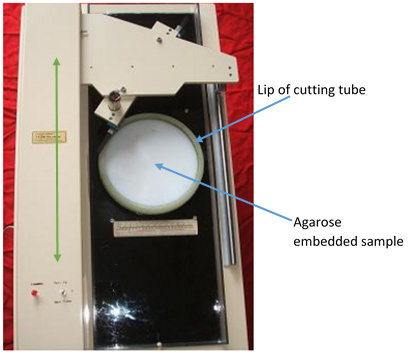
\includegraphics[width=0.5\textwidth]{VF900}
		\caption[VF900 Caption]{Precision Instruments VF900\footnotemark\label{precision_instruments}. Green arrow shows direction of cutting action.}
		\label{VF900}
	\end{figure}
	\footnotetext{http://www.precisionary.com/vf900 [Accessed 08/04/16]}
	
	\newpage
	\subsection{Intermediate Sectioning}
	\label{sectioning_smaller}
	
	The initial sectioning (coronal slicing) of the brain results in \SI{13}{\centi\meter} x \SI{9.3}{\centi\meter} x \SI{0.5}{\milli\meter} slices. These slices must then be further sectioned into blocks which can undergo the post fixation and staining processes detailed in Section \ref{postfixation} before progressing to final sectioning and imaging. The limiting size of these blocks is what will fit on an ATUMtome. \SI{3.5}{\milli\metre} x \SI{2.5}{\milli\meter} seems to be towards the upper limit of what ATUM is capable of reliably sectioning \cite{hayworth2014atum} and so these are the dimensions which will be aimed for.
	
	There do not appear to be any commercially available devices which are intended to produce high quality sections from a slice of this size at the time of writing. The closest possible device appears to be the McIlwain Tissue Chopper. However, this device is incapable of accommodating the initial dimensions of our slice. Because of this it has been necessary to determine what custom solutions may be possible.
	
	\begin{figure}[!h]
		\centering
		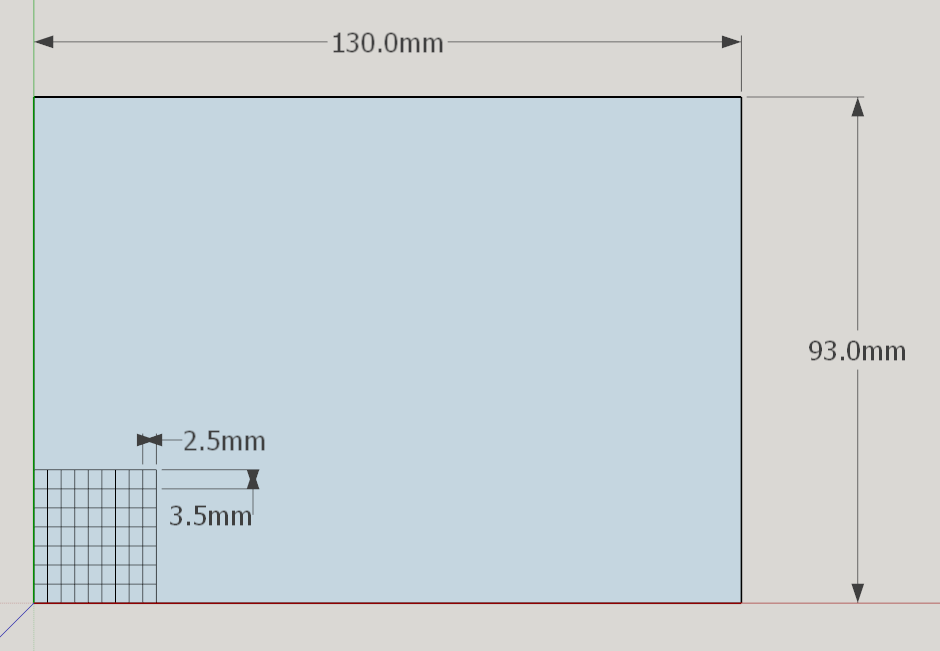
\includegraphics[width=0.5\textwidth]{brainslice}
		\caption{Diagram to show how the blocks need to be sectioned from the brain slice.}
		\label{brainslice_diagram}
	\end{figure}
	\subsubsection{Focused Ion Beam Milling (FIB)}
	\label{sectioning_smaller_FIB}
	
	As mentioned in Section \ref{sectioning_smallest_FIB}, FIB milling has widely been used in the semiconductor industry for fabrication but has only been used for removal of a block face in the preparation of biological samples. We see no reason why this technology could not be adapted for this task. Such a device would closely resemble a traditional horizontal CNC milling machine, however, instead of a milling cutter it would have a focused ion beam. This would mean that the beam could move in both X and Y dimensions and so allow for the necessary grid pattern to be milled into our brain slice.
	
	As in Section \ref{sectioning_smallest_FIB} the biggest problem with FIB milling is the time it takes to perform. To judge whether or not FIB milling could be an appropriate solution it is important to estimate how long it would take to divide each slice into blocks. If we are minimising tissue loss, then the aim would be to mill only \SI{5}{\nano\meter} of tissue away between blocks as this is near minimum milling width which has been reliably achieved \cite{knott2008serial}. This would mean that the total volume of tissue which needed to be removed for each block (except the last column and row) would be approximately:
	
	\begin{figure}
		\centering
		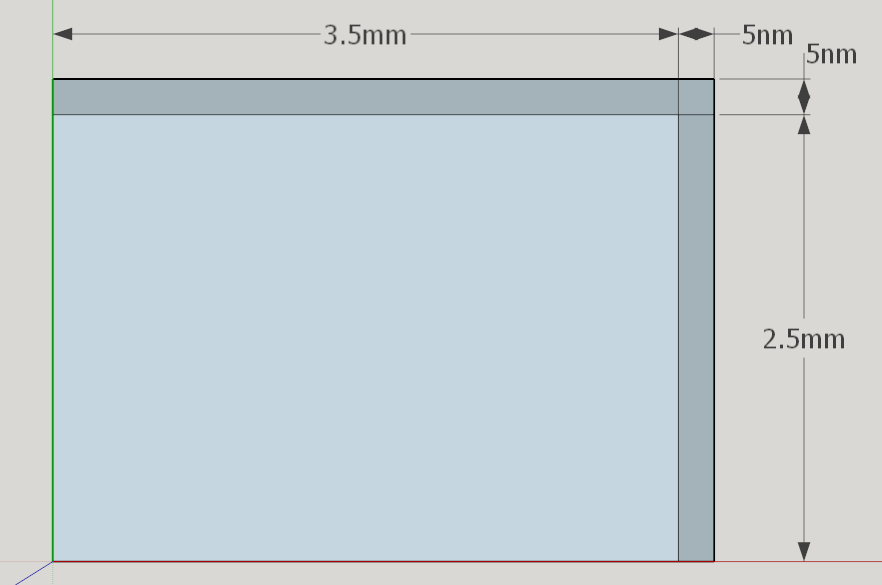
\includegraphics[width=0.5\textwidth]{brainblock}
		\caption{Illustration of FIB milling volume per block (not to scale).}
	\end{figure}
	
	\begin{align}
	Milling\ Volume\ per\ Block &= (3.5\times10^{-3} + 5\times10^{-9}  2.5\times10^{-3}) \times 5\times10^{-9} \times 0.5\times10^{-3} \nonumber \\
	&= 1.50\times10^{-14}\ m^3  
	\end{align}
	
	If we assume that the rate of milling of \SI{75}{\second} for a block which is \SI{900}{\micro\meter\square} x \SI{40}{\nano\meter} achieved in \cite{knott2008serial} can be reproduced and that milling time is proportional to milling area, we can determine approximately how long it would take to mill an entire slice.
	
	\begin{align}
	Time\ per\ Block = \frac{1.50\times10^{-14}}{900\times10^{-12} \times 40\times10{-9}} \times 75 = 31250 seconds = 8.7hours \\
	Time\ per\ Slice = \frac{13\times10^{-2} \times 9.3\times10^{-2}}{3.5\times10^{-3} \times 2.5\times10^{-3}} \times 8.7 = 12021hours
	\end{align}
	
	Knott et al  found that the maximum cutting depth of FIB milling is limited by the focus of the beam, with greater milling depths resulting in greater damage to the cut surface due to the beam becoming less focused \cite{Knott2011}. It is not clear whether this limitation might make it infeasible to cut through a \SI{500}{\micro\meter} slice of brain tissue using FIB.
	
	\subsubsection{Custom Tissue Chopper}
	\label{sectioning_smaller_tissuechopper}
	
	Another option which must be considered is a simple tissue chopper like those discussed in Section \ref{sectioning_small_tissuechopper}. However, as has already been pointed out there are no appropriate commercial solutions. It would, therefore, be necessary to either purpose build a tissue chopper from the ground up or modify an available model. As mentioned previously the  McIlwain Tissue Chopper\footnote{https://www.tedpella.com/vibratome\_html/10180.htm [Accessed 11/04/16]} seems to be the closest thing to what we need. However, it has a few limitations. Firstly, it is designed to use a standard razor blade which is typically about \SI{40}{\milli\meter} long and so unable to section our \SI{13}{\centi\meter} x \SI{9.3}{\centi\meter} slices with a single cut. Secondly, the device is designed to have a maximum slice thickness of \SI{1}{\milli\meter}, which is too narrow for our needs. Thirdly and finally, the provided cutting table is unable to accommodate our slices.
	
	The first problem should not be difficult to solve. It should not require heavy modification to allow for a much longer knife be mounted to the chopper such as the tungsten carbide knives provided by Delaware Diamond Knives\footnote{http://www.ddk.com/tungsten-carbide-knives.php [Accessed 11/04/16]}. Normally the machine advances the sample at a linear rate and drops the blade onto it at a fixed frequency. It should also not be infeasible to modify the advance system of the device to be capable of progressing in both \SI{2.5}{\milli\meter} and \SI{3.5}{\milli\meter} steps rather than at a controllable constant speed. Finally, it would be necessary to expand the cutting platform to have a diameter of at least \SI{13}{\centi\meter}. If these modifications are not possible it should be possible to have a similar device manufactured to our specifications.
	
	Using this technique, the actual time it takes for the blade to cut the sample would be negligible. The more important figure would be the advance speed. The McIlwain Tissue Chopper is capable of making 200 cuts per minute, if we assume that with modifications to the advance system our device is capable of operating at 10\% of that speed or one cut every 3 seconds. This would result in a very reasonable maximum advance rate of \SI{1.17}{\milli\meter\per\second}. Assuming that this advance rate is achievable and an additional 5 minutes is allowed, once all the cuts in one direction have been completed for carefully ordered collection from the water bath of the slices and rotation through 90\textdegree. This would result in a total cutting time per slice of:
	
	
	\begin{align}
	Total\ Number\ of\ Cuts &= \frac{130}{2.5} + \frac{93}{3.5} = 78\ cuts \nonumber \\
	Cutting\ Time &= \frac{Total\ Number\ of\ Cuts}{Cuts\ per\ Minute \div 60} + (5\times60) \nonumber \\
	&= \frac{78}{20 \div 60} + (5\times60) = 534seconds		
	\end{align}
	
	This is a much more manageable rate of cutting compared a FIB method and would certainly not bottleneck any other part of the process. 
	
	\subsubsection{Custom Vibratome}
	\label{sectioning_smaller_vibratome}
	
	Commercially available vibratomes have three major problems which make them unsuitable for our intended purpose. The first of these two problems is that the maximum section thickness which can be cut is \SI{1}{\milli\meter}, whereas we need up to \SI{3.5}{\milli\meter} so this will need modification. Commercially available vibratomes such as the Leica VT1200 S can only fit \SI{70}{\milli\meter} x \SI{40}{\milli\meter} specimens. This is clearly too small to fit an entire brain slice but a custom-made machine will do so. The other main issue with conventional vibratomes is that the cut orientation is not appropriate for our needs, since they are designed to take thin slices from small blocks of tissue whereas our intended use is to take very long thick slices. My design proposed for the modification is demonstrated in Figure \ref{custom_vibratome}. In this figure the horizontal blade would slice through the agarose above the brain slice in order to present an overhang similar to that which is present in a microtome. This knife would then retract in order to allow for the blade which is orientated vertically to advance and remove a long ribbon from the agarose block which would then fall into a water boat below for collection. These ribbons, collected from the water boat in a carefully ordered sequence, could then be mounted in a similar fashion and sliced again to leave the small blocks to be mounted on ATUMtome.
	
	\begin{figure}
		\centering
		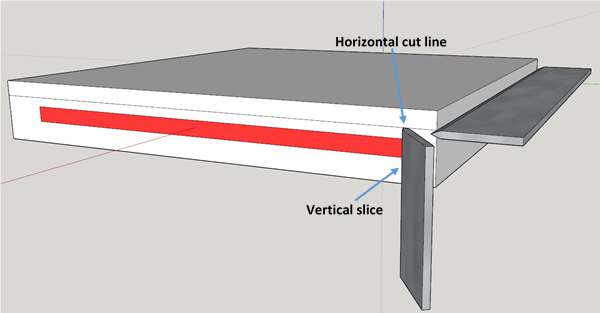
\includegraphics[width=0.7\textwidth]{custom_vibratome}
		\caption{Red is the brain slice. White is agarose in which the slice is embedded.}
		\label{custom_vibratome}
	\end{figure} 
	
	If we assume that our custom vibratome will have similar cutting speeds to the Leica VT1200 S\footnote{http://www.leicabiosystems.com/histology-equipment/sliding-and-vibrating-blade-microtomes/vibrating-blade-microtome/details/product/leica-vt1200-s/ [Accessed 08/04/16]} and add a margin of error in order to account for the increased number of moving parts, then it is possible to obtain an estimate for the time it would take to section a single slice of brain. The range of VT1200 S cutting speeds is \SI{0.025}{\milli\meter\per\second} to \SI{2.5}{\milli\meter\per\second}. We will select a speed towards the lower end of this range for the blade orientated vertically (\SI{0.5}{\milli\meter\per\second}) in an attempt to reduce pressure on the specimen and so produce a higher quality cut. The horizontal blade may advance much more quickly as it is only cutting through agarose (\SI{2.5}{\milli\meter\per\second} whilst cutting). The blade may however advance much more quickly when it is not cutting material. We will also assume that for each cut that the horizontal blade makes it must advance and retract a total of approximately \SI{60}{\milli\meter} and that this will take a total of 10 seconds. Finally we will assume that the agarose block, which must be larger than the brain slice, will be \SI{140}{\milli\meter} x \SI{140}{\milli\meter}.
	
	\begin{align*}
	Number\ of\ Cuts &= \frac{130}{2.5} + \frac{93}{2} = 78\ cuts \nonumber \\			
	\end{align*}
	\begin{align}
	Time\ per\ Cut &= \frac{Vertical\ Cut\ Length}{Vertical\ Cutting\ Speed} +\frac{Horizontal\ Cut\ Length}{Horizontal Cutting\ Speed} + Traverse\ Time \nonumber \\
	&= \frac{140}{0.5} + \frac{3.5}{2.5} + 10 = 291\ seconds \nonumber \\
	Total\ Cutting\ Time &= Time\ per\ Cut \times Number\ of\ Cuts = 291 \times 78 = 22698\ seconds	\nonumber \\
	&= 6.3\ hours
	\end{align}
	
	This is significantly longer than sectioning of a slice would take using a tissue chopper, however, at this cutting speed this stage of the process would still not be the limiting factor in how quickly the brain can be processed. 
	
\subsubsection{Discussion}
\begin{table}[h]
	\centering
	\caption{Comparison of intermediate sectioning techniques.}
	\label{intermediate_sectioning_techniques}
	\begin{tabular}{|l|l|l|l|l|}
		\hline
		\textbf{Method}       & \textbf{Speed} & \textbf{Cut Quality} & \textbf{Ease of Use} & \textbf{Practicality} \\ \hline
		FIB Milling           & Very Low       & Excellent            & High                 & Low                   \\ \hline
		Custom Tissue Chopper & Very High      & Poor                 & High                 & Very High             \\ \hline
		Custom Vibratome      & High           & Very Good            & Low                  & High                  \\ \hline
	\end{tabular}
\end{table}

FIB milling seems like a very attractive option due to its extremely low specimen loss and damage. However, the extremely slow cutting rate and the significant question over whether it is possible to reliably and accurately mill through a \SI{500}{\micro\meter} slice of brain make it unsuitable for our uses.

The tissue chopper is also an attractive option. It provides very fast sectioning as well as being easy to use and being a relatively simple machine to produce or modify. It should be noted, however, that a cutting speed as faster as the tissue chopper's is not required due to other bottlenecks within the process limiting the rate at which the slices are required to be sectioned. Finally, the poor section quality inherent to tissue choppers when compared to a vibratome device means that we feel that the vibratome, despite being a much more complicated device, is a more suitable solution.

\newpage
\pagestyle{john}
\section{Recording Technologies}
\label{RecTec}
\subsection{Introduction}
The ultimate objective of the technology that we choose to image the human brain will be to produce images with great enough resolution for our algorithms to identify synapse locations. The reasoning behind this is the theory that 'we are our connectome'\cite{seung2013connectome}, namely, the brain can be summarised through recording the totality of its synaptic connections, as suggested in the introduction. However, neurons are not alone in the brain, and its understood that microglia, astrocytes and oligodendrocytes all influence neural connectivity \cite{fields2015glial}. The resulting uncertainties lead us to choose a method that allows for imaging to be as precise as possible, minimising the chance of not capturing some feature of currently unknown importance. We will be producing an extensive set of data, hopefully representative of all major information and processes, currently most will only be used to provide identifying features of synapses but we have the capability to extend our identification algorithms should the need arise. Methods of classifying synaptic locations (see below, section 7) require identifiable sub-cellular structures, therefore to reliably detect them we'll need 3-5 nm\cite{Briggman2012154}\cite{mikula2015high} resolutions. We will also be required to align images; this will allow us to produce a 3D 'block' of brain tissue so that full synapse structures can be identified. Finally, due to multiple constraints including as time, money and security\footnote{If reanimation became a reality customers need assurance only we will have access to their information.} we  will aim to automate the entire digitization process. As has already been stated we will be using scanning electron microscopy. This section will establish the reasoning for using this method whilst providing a record of alternative techniques should further developments render them preferable. 

\subsection{Magnetic Resonance Based Methods}
\subsubsection{MRI}
The human brain is approximately 73\% water\cite{mitchell1945chemical}, therefore contains many hydrogen protons. These act similarly to bar magnets when introduced to a high powered magnetic field and begin to line up with it. The protons also begin to precess at the Lamour frequency $\omega_{\o}$, which is related to the field strength $\mathsf{B}_{\o}$ given by equation~\eqref{precess}:
\begin{align}\label{precess}
	\omega_{\o}=\gamma\mathsf{B}_{\o}
\end{align}


Where $\gamma$ is the gyromagnetic ratio. An RF pulse of the same frequency can tip these protons to align at $90^{o}$ to the field and precess in phase. Now that the proton is in a high energy state we can start to listen for signals returning from the brain, notated T1 and T2 relaxation. T1 being the release of RF when the protons flip back in line with the field, T2 the slow proton de-phasing which results in decaying transverse magnetization. \cite{weishaupt2008does}\\
For an MRI machine with a magnetic field strength of 3T, we'd be getting isotropic voxel resolutions of around 1mm for T1 weighted images and 0.7mm for T2. \cite{fan2016mgh} Unfortunately this is nowhere near the resolutions we require, so despite having the huge benefit of being non-invasive, magnetic resonance imaging must be discounted.\\
\subsubsection{fMRI}
Functional MRI relies on a signal similar to the T2 signal called T2*, the difference being much faster decay of transverse magnetization due to irregularities in the magnetic field. These occur around locations of blood flow, when neurons are firing a proportionally higher blood flow occurs around the area and so affects the signal and allows for imaging. However, fMRI still only produces isotropic voxel resolutions of around 1mm at a 3T magnetic field strength. MRI is being used to generate a 'functional' connectome which aims to provide insights into the interacting systems of anatomically connected areas and brain responses to stimuli\cite{van2010intrinsic}. It may be useful to record this alternative form of connectome, especially for the ultimate goal of future reanimation in which we do not yet know the full requirements for the process. Unfortunately, the uncertainty of its usefulness combined with extra cost, time, money and the risk of damage to the patient's brain through tissue heating result in our current rejection of the technique.\\
\subsubsection{MRFM}
An alternative method, magnetic resonance force microscopy, uses the principles of MRI, but with an ultra-sensitive cantilever to which samples are attached as demonstrated in Figure \ref{MRFMPic}. A magnetic tip 3 dimensionally scans over the sample whilst a coil produces an RF pulse. The realignment of protons causes a periodic force on the cantilever, allowing reconstruction of proton density. This technique leads to spatial resolutions of around 4 nm by creating and extremely high magnetic field gradient close to 4 million T/m around the tip. However, research currently consists of an individual tobacco mosaic virus of size 0.8$\mu$m $\times$ 1.3$\mu$m which is much smaller than the samples we are considering. This would mean an excessive amount of preparation in terms of cutting. Furthermore, scanning of a 50 nm x 50 nm area can take in the region of 32 hours which is simply too slow\cite{park2012semi}. I would also question the stability of the microscope, as given it would need to be used for extended periods of time, any tremor or disturbance could influence the attonewton forces it detects and subsequently corrupt the data set. 
\begin{figure}[htb!]
	\centering
	
	
	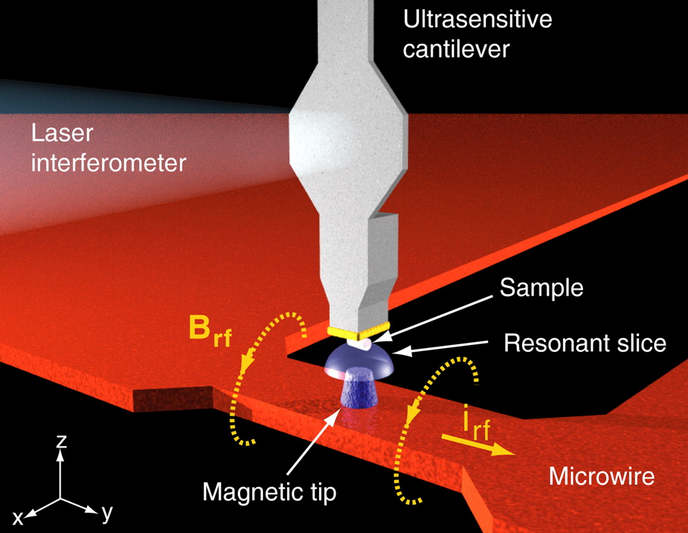
\includegraphics[width=0.6\textwidth]{MRFM.PNG}
	\caption[A demonstration of how a magnetic resonance force microscope works]{\centering \label{MRFMPic}A demonstration of how a magnetic resonance force microscope works\cite{Degen03022009}}
	
\end{figure}

\subsection{Light Based Methods}
Light microscopy methods generally rely on fluorescent proteins; excitation light is shone on the specimen and these proteins proceed to emit a lower energy and longer wavelength light. A filter separates out this emitted light, allowing for observation. A primary issue with this method is resolution. As visible light is used, we are limited by its diffraction limit leading to a minimum x-y plane resolution of around 200 nm \cite{hell1994breaking}. This is not good enough for our purpose and even with confocal microscopy in which a pin hole rejects out of focus light before it reaches the detector, we only get around a 1.4 factor improvement \cite{lauterbach2012finding}. Resolutions in the z plane are even worse reaching only around 700 nm. Although, taking ultra thin sections clearly improves upon this especially when combined with array tomography.\footnote{However this requires the inclusion of SEM.} \cite{micheva2007array} \\
\subsubsection{STED}
Methods have been discovered that break this diffraction limit, such as stimulated-emission-depletion (STED) fluorescence scanning microscopy. Excitation occurs as normal through the use of a laser, however a second laser which is split into 2 beams is also shone on the sample. This second beam depletes the excited state before florescence has occurred in an immediate area around the center of excitation (A zero point). This has the effect of increasing the resolution \cite{hell1994breaking} and is compatible with a wide range of fluorescent probes \cite{dani2010new}. Extending this theory into the third dimension by adding a second STED laser with a time delay to prevent interference can lead to isotropic spatial resolutions of 40 nm. Further improvements can be made to reduce the time of imaging by simply parallelising (currently shown to a factor of 2000 times) the excitation and fluorescence inhibition (STED) beams\cite{bergermann20152000} through the use of two orthogonally crossed standing waves. There is no notable drop in resolution and the area that can be imaged at once is drastically increased. An issue that can arise from the use of high intensity laser sources is photobleaching which renders the sample unable to fluoresce and ultimately leads to a loss of data. To solve this issue one can use a different type of fluorescent protein, ones which have a deactivated as well as a ground and activated state. By deactivating certain proteins rather than simply driving them to their ground state (depletion), the majority can be protected\cite{strack2016imaging}. Using parallelisation is also beneficial in the reduction of photobleaching due to steeper intensity gradients than in the standard method, leading to 15.4 times less energy per zero\cite{bergermann20152000}.\\
\subsubsection{STORM/PALM/FPALM}
A different approach, alternatively named STORM/PALM/FPALM by separate labs relies on photoactivatable fluorescent proteins such as mEos2 \cite{dani2010new} in a similar way to those used to prevent photobleaching in STED. One wavelength of light can be used to deactivate the fluorophores whilst another is used in the imaging process. The sample can then be iteratively activated and sampled to reveal each fluorophore location, finally everything is combined to form a super high resolution image. This can be extended into the third dimension by using a cylindrical lens to produce differences the x and y focusing allowing lateral positioning to be determined. Resolutions can be around 25 nm axially and 50 nm laterally\cite{huang2009super}.\\

\subsubsection{Brainbow}
We have discussed a few methods of using light based imaging demonstrating that they are rapidly approaching resolutions that would be acceptable. Brainbow is the use of multiple 'primary' coloured fluorescent proteins, in much the same way as RGB TV channels, to produce a spectrum by using varying combinations. This spectrum is intended to be used to map out an entire connectome, up to 90 different colours means adjacent neurones can be differentiated and entire neural circuits can be traced out.\\
By crossing different lines of genetically modified mice with different XFP's, patches of each colour can be found throughout their brain. However, this does not result in enough variation in colours so two different methods were introduced: Brainbow-1 and Brainbow-2. To describe these we must first introduce Cre-lox technologies, Cre recombinase and a loxP recognition site are found naturally in the P1 bacteriophage. Cre recombinase catalyses the recombination of two loxP sites which are located on DNA, they then align in parallel and Cre proteins cause one or multiple of the following events to occur. Either inversion of the region of DNA between sites, deletion of this region or trans-location between separate DNA strands\footnote{http://blog.addgene.org/plasmids-101-cre-lox [Accessed 02/02/2016]}. In Brainbow-1 red fluorescent protein is expressed unless Cre deletion action occurs resulting in yellow fluorescent or cyan fluorescent expression as seen in Figure \ref{Brainbowpic}. Later orange fluorescence was also included resulting in a four colour cellular array. \cite{Livet2007}\\
Brainbow-2 combines Cre deletion and inversion, the use of two invertible DNA segments in tandem allowed multiple different colours through the large number of combinations possible\cite{Livet2007}. 
\begin{figure}[h]
	\centering
	
	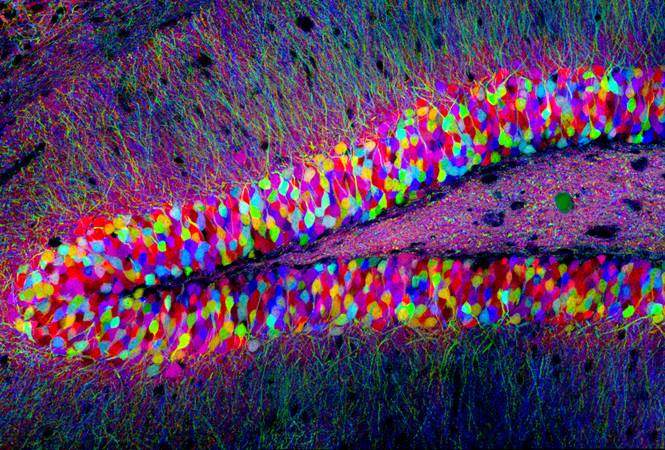
\includegraphics[width=0.8\textwidth]{Brainbow.jpg}
	\caption[An example of a Brainbow-1 mouse brain image, taken from a layer of the hippocampus]{\centering \label{Brainbowpic}An example of a Brainbow-1 mouse brain image, taken from a layer of the hippocampus\footnotemark}
	
\end{figure}
\footnotetext{http://www.cell.com/pictureshow/brainbow [Accessed 05/03/2016]}

Once the mice had been genetically modified a confocal microscope was used to image part of a Brainbow-1 brain. As expected a wide range of colours were observed and axons were not only distinguishable, but also able to be traced.
Unfortunately, from colour variation alone 1.1\% of all presynaptic terminals were lost, any loss of synaptic data is taken very seriously and this is quite a significant amount\cite{Livet2007} after losses in cutting. There was also evidence of fluorophore photoinstability and the 'default' state tended to be much more commonly expressed than the others. A third Brainbow technique was developed to address some of these issues. By screening which fluorophores were used immunostaining became possible and new derivatives allow direct trafficking of the proteins to the cell membranes \cite{cai2013improved}. We are still resolution limited, especially with confocal microscopy which leaves this method fairly redundant for now. We could possibly hope to increase resolutions to resolve subcellular structures and synaptic junctions that are currently too small through the use of the super resolution LM methods discussed above. However, this would require the use of compatible proteins which for now we can't be sure of. Regardless we would still be under the limitations of those methods.

\subsubsection{ExM}
A recently developed technique Expansion Microscopy, shows great premise for expanding the capabilities of all microscopy methods. Rather than increasing the optical resolution, tissue is physically expanded, currently by a factor of 4.5, using a swellable polymer network. Despite having variations in the amount of polymerisation throughout the tissue, at a nanometre scale they average out resulting in an isotropic image. The initial researchers used a three part fluorescent label which consisted of a chemical fluorophore, a methacryloyl, and an oligonucleotide. This shows an example of what can be used during the expansion process, more research of this type needs to be produced, or perhaps be performed by ourselves in order to ensure adequate labelling of all synapses and sub cellular structures.
Currently this arrangement demonstrates that the method supports resolutions in brain tissue of around 70 nm laterally and 200 nm axially, using confocal microscopy and GFP markers. Whilst there is not presently a wealth of information on the topic, especially concerning the effects of different stains, markers and preservatives the method is definitely worth monitoring as it could provide extremely detailed images. The greater the detail of the image, the easier it is for our algorithms to detect synapses. Therefore, the is the possibility our operation could not only be performed faster but with more precision and reliability. \cite{chen2015expansion}\\

One source has found the initial researchers are exploring greater expansion factors of up to 15-20$\times$. This would lead us to at least to a 20 nanometre lateral resolution using our confocal microscope.  Synaptic markers have been mentioned by the researchers under the assertion that samples would need to be very thin, which as we have shown in section 1 we are already prepared to do. However, there are doubts as to the uniformity at further scaling, and with alternately prepared samples as some structures may not expand as easily, or in the same fashion as others. They have even implied issues specifically with pre and post synaptic membranes which obviously would be very detrimental to our imaging process should they become too distorted to identify. These issues are being addressed through attempts to stiffen samples, however in its current state expansion microscopy would be a large risk to take. Therefore, we must currently disregard the method whilst bearing in mind that expansion microscopy could very well bring light microscopy to the forefront of nanoscale resolution in the near future. \cite{marx2016optimizing}

\subsubsection{Discussion}
As we've seen LM resolutions can be further improved, however there is an issue we have not addressed - fluorescent labelling in the context of our client's brain. Different techniques such as dye injection, immunolabelling, or fluorescent protein fusions can be used. These markers will label specific molecules, bearing in mind for the two super resolution methods, only certain ones will work. Many techniques for introducing them such as in the Brainbow method require genetic modification pre-birth, this is clearly not possible. As an alternative gene therapy could be used to introduce new genetic material into cells; in this case, to create a fluorescent protein. It is not possible to just insert a new functioning gene into a cell, we must make use of a genetically engineered vector such and a retrovirus. The vector can be injected into the tissue where it is taken up by individual cells in which the gene will be delivered\footnote{https://ghr.nlm.nih.gov/primer/therapy/procedures [Accessed 10/03/2016]}. Unfortunately there are still many technical challenges to overcome and sufficient delivery too all cells would not be possible. 

Furthermore, most synapses will bind to very few fluorophores with random fluctuations occurring throughout the tissue, this can lead to larger synapses overshadowing the smaller ones \cite{mishchenko2010optical}and thus unacceptable loss of data.


\subsection{X-ray Methods}
\subsubsection{Hard X-rays}

The short wavelength of x-rays mean that they can penetrate through relatively thick samples of greater than 1 micron, largely reducing the amount of sectioning necessary. A new technique utilising nanofocusing optics (the multilayer Laue lens) allows for theoretically sub-nanometre resolutions. However it has currently only been able to demonstrate down to 11 nm. The focused x-rays are raster scanned across the sample and x-ray fluorescent photons are analysed by an energy-dispersive detector. Simultaneously a pixel-array detector captures the transmitted beam signal and an algorithm is used to produce absorption-contrast and phase-gradient images. These are sensitive to heavy metal stains and compositional variations respectively\cite{yan2016multimodality}. Issues that arise are the damage due to radiation (although none were shown when imaging a chromosome), the size of the machinery (a 250m long imaging and coherence beamline) and that the staining used can alter the morphology of structures. Dwell times of around 1 second are also fairly slow compared to the 100 ns of the MultiSEM 505 (see below Section \ref{EMChemRef}). It is thus suggested that this method is used complementary to others, but due to cost and time that is not practical for our objectives.



\subsection{EM Based Methods}
\label{EMChemRef}

Electron microscopy has been a stable field for high nanometre resolution images for many years, the two main categories being Transmission and Scanning Electron microscopy.  From the outset both provide excellent resolution due the wavelength of electrons being much lower than light at 39pm to 3.9pm at energies of 1 and 100 keV respectively\cite{denk2012structural}. A number of experts in the field of neuroscience, including  Kenneth Hayworth, Jeff Lichtman and Bobby Kasthuri, have shown EM can provide images with identifiable synapses and vesicles. Large manually labelled data sets have been produced and are available for download and use, we can utilise such data to train machine learning algorithms.  

\subsubsection{TEM}
Transmission Electron Microscopes consist primarily of an electron gun, electromagnetic lenses and a charge-coupled device camera, all contained within a vacuum in which the specimen will be placed. Inside the gun there is a filament and an anode, when a large positive potential is applied across them, electrons are ripped from the former and pass through a small hole in the latter. This provides a fine beam of electrons at extremely high velocities of up to three quarters the speed of light for an accelerating voltage of 300 kV\cite{beniac2010introduction}. There are a few different types of filament, these vary in price, level of vacuum requirements, lifespan, stability and brightness. Lifespan is clearly an issue that needs to be thoroughly considered; whilst a tungsten filament would provide suitable levels for most of the above factors, its short lifespan in comparison to LaB$_{6}$ and field emission sources may severely hinder any attempt at automation. 

\begin{center}
	\captionof{table}{Comparison of EM filaments} \label{tab:filaments}
	
	\begin{tabular}{ |c|c|c|c| } 
		\hline
		Filament      & Lifespan (h) & Emission Current Density (A/cm$^{2}$) & Brightness (A/(cm$^{2}$.sr.kV))\\ 
		\hline
		Tungsten          & 100         & 3		& $10^4$     \\ 
		LaB$_6$        & 	>1000       & 30     	&  $10^5$\\ 
		ZrO/W (FEG) & 	>5000       & 5300     & $10^7$\\
		\hline	
	\end{tabular}
\end{center}
\small{Source: https://www.microtonano.com/EBS-Tungsten-EM-Filaments.php}\\
\normalsize
The electromagnetic lenses essentially focus the electron beam, through small gaps in their magnetic circuits, onto the sample allowing the camera below to detect transmitted electrons. The main source of scattering in organic samples is due to the thickness and composition of the material encountered, using positive stains increases scattering around organelles whilst negative does the inverse\cite{egerton2006physical}.  

TEM seems satisfactory, having well defined staining techniques\cite{knott2008serial},\cite{egerton2006physical}and easily reaching resolutions of 1 nm \cite{EMFundementals}. Yet the time to image a section and the size of section able to be imaged are hugely limiting factors. To improve upon these a TEM camera array can be used (TEMCA) which, as implied, is the addition of extra high speed CCD cameras whose images are mosaiced together into one larger image. \cite{bock2011network} As indicated in table  \ref{tab:imagetime}, this clearly is still not scalable to a human brain. 



\subsubsection{SEM}
Scanning Electron Microscopes contain mostly the same components as in TEM, minus a few electromagnetic lenses below the sample. These are not needed, as the electrons do not need to pass through the sample (although can also be used). Instead SEM detects back scattered electrons and/or secondary electrons (although these are the major type of detection - there is also X-rays and visible light photons), these possess low energies meaning only those emitted very close to the surface get detected. Rather than a single wide beam as in TEM, a very narrow beam is scanned across the sample with low accelerating voltages. Three types of detector are regularly in use. A scintillator uses the light produced when an electron hits a fluorescent screen and converts it to an electrical signal via a photomultiplier tube. Alternatively, semi-conductors can be used, either with an amplifier to detect incoming electrons, or by monitoring the current absorbed by the sample through monitoring the induced current across the semi-conductor junction. There are many advantages to be had via SEM, such as the resolutions of around 1  nm being easily acceptable whilst requiring lower voltages (hence damage is much less likely). The size of samples able to be placed within these machines also tends to be much larger \cite{beniac2010introduction}. In terms of imaging time SEM is actually still much too slow, given a currently top of the range microscope could take as long as 2.5 hours to image 1mm$^2$(at 4  nm resolution)\cite{ZeissPres}.This brings us onto Multi-beam scanning electron microscopy.



\subsubsection{MultiSEM}
\label{recording_EM}
Rather than using a single electron beam multiple in parallel can be used within the same optical column, each having their own detection unit. This allows for much larger areas to be imaged. Zeiss produce two Multi-Beam SEM's the 505 with 61 beams and the 506 with 91 beams, both use a Schottky emitter. The array of beams is scanned across the sample in a hexagonal beam pattern which reduces electron optical aberrations, then a magnetic beam splitter separates secondary electrons for detection. The hexagons can be used to form a mosaic and display a large section as shown below in Figure \ref{fig:BeamsSEM}. Imaging times can be decreased by a factor directly proportional to the amount of beams used (as each individual beam is scanning an area equivalent to a standard SEM scan in the same amount of time). One of the major scaling issues is the huge amount of data this generates, thus the transfer to storage must also be highly parallelised \cite{eberle2015multiple}. \\


\begin{figure}[H]
	\centering
	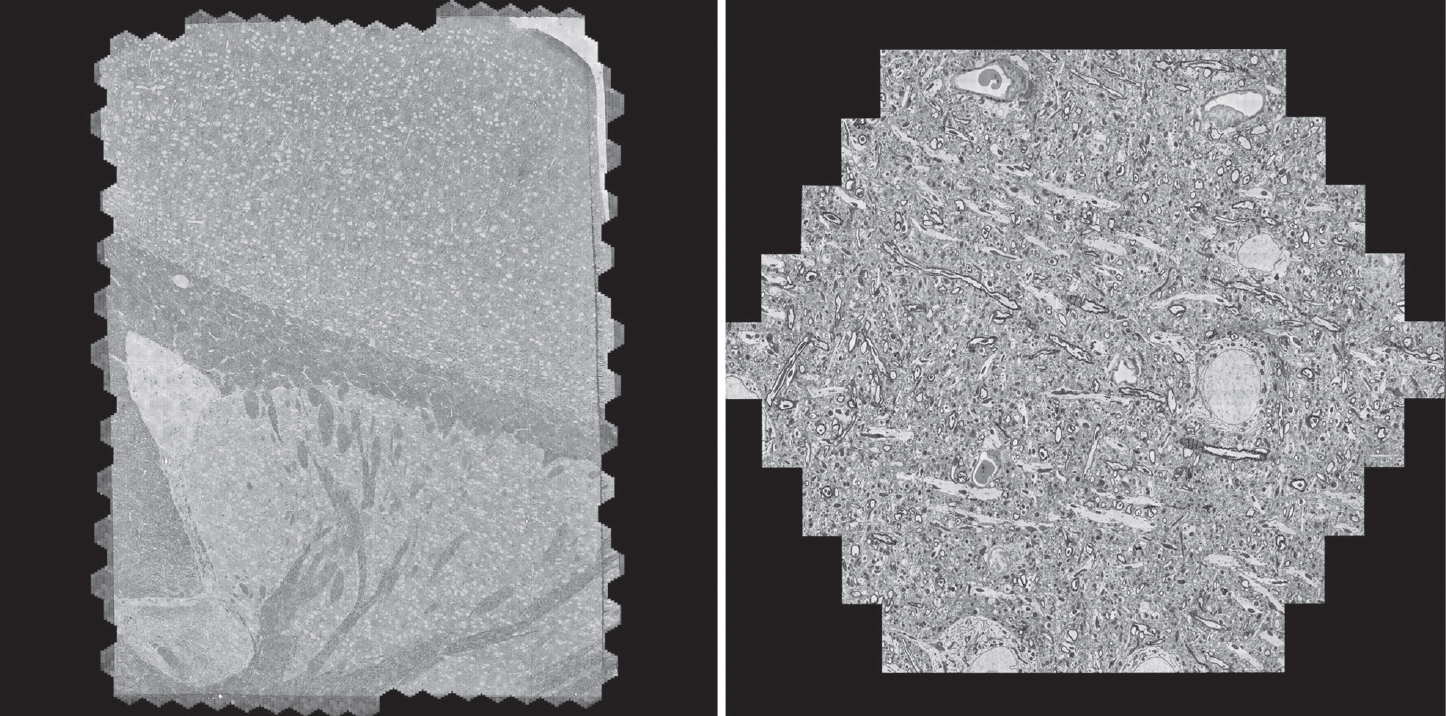
\includegraphics[width=\textwidth]{BeamsSEM}
	
	\caption[Mosaic and hexagon pattern of beams (Sample by Jeff Lichtman and Richard Schalek, Harvard University)]{\centering \label{fig:BeamsSEM}Mosaic and hexagon pattern of beams (Sample by Jeff Lichtman and Richard Schalek, Harvard University)\protect\cite{eberle2015multiple}}
\end{figure}


In table \ref{tab:imagetime} we can form a rough idea of the time improvements the 505, 506 and TEMCA give relative to each other, which is clearly fairly substantial. Calculations are based on an estimated brain volume of 1900cm$^3$\cite{brain_size} and slice thickness of 30  nm as proposed in sectioning (\ref{sectioning}), these rough estimates are purely for the microscopes image time. They will be expected to run autonomously for 24 hours a day in order to minimise the temporal bottleneck imaging creates. As an example, for the MultiSEM 506 see Equation \ref{ScanTime} 

\begin{align}
Brain\ Scan\ Time &= \frac{Total\ Brain\ Area}{Approx\ FOV} \times FOV\ Scan\ Time\nonumber\\
&\approx \frac{63,000}{2.55\times10^{-8}}\times1.4s \nonumber\\
&= 3.45\times10^{12} s \nonumber\\
&\approx 110,000\ years
\label{ScanTime}
\end{align}
\clearpage
\begin{center}
	\captionof{table}{Comparison of EM Imaging Times} \label{tab:imagetime}
	
	\begin{tabular}{ |c|c|c|c| } 
		\hline
		& TEMCA \cite{Briggman2012154}  & MultiSEM 61 Beam \cite{ZeissMulti} & MultiSEM 91 Beam\cite{ZeissMulti} \\ 
		\hline
		
		Approx FOV(m$^2$)  &  4$\times10^{-10}$     & 7.8$\times10^{-9}$         & 2.55$\times10^{-8}$      \\ 
		Scan Time per FOV (s)   & 1 & 	1.3      & 1.4      	\\ 
		Total brain scan time (years) & 	 5.0$\times10^{6}$       & 3.6$\times10^5$     & 1.1 $\times10^5$\\
		\hline	
	\end{tabular}
\end{center}


As can be seen, the MultiSEM 506 offers by far the best imaging time and therefore is the clear choice; for a reasonable time of ~10 years (allowing nearly a year for unexpected delays) an entire brain scan will require around 12,000 machines.




Further benefits come from the use of the MultiSEM,  it has been designed with automation in mind and comes provided with software that fully automates the scanning procedure (ZEN). Although we may require some additional programming (i.e integration with WaferMapper to reduce time between scans see Section \ref{WaferMapper}) to suit our application it is straightforward and includes smart auto tuning routines. The requirements for this automation include a light microscope to allow for sample alignment via fiducial markers, however provided a constantly moving pipeline this should not significantly delay our pipeline. These microscopes have already seen use in the neuroscience community by Jeff Lichtman and Winfried Denk, Zeiss have worked closely with these researchers to provide optimisations. These include being designed to run 24/7 and an airlock for quick specimen transfer\cite{ZeissMulti}. 

In order to remove the need for an operator to change samples which would hinder 24/7 operation, we intend to use a robotic arm. Industrial robotic arms are available online\footnote{https://www.densorobotics-europe.com/en/robots,http://www.globalrobots.com/ [Accessed 05/03/2016]} for around \pounds6000-\pounds10,000, and we can assume \footnote{Communications with Dr Eberle} that the changing time for samples can be achieved with said arms in around 5 minutes (as we are limited by the airlocks compression time). Given the max sample size that can held within the MultiSEM machine is 10x10cm  \cite{ZeissMulti} and assuming at least 50\% of that area is taken up by brain tissue the time added by the arms is negligible (for 12,000 machines few changes are necessary). 

Given we now have our chosen microscope we can begin to estimate space requirements. Zeiss estimates an area of 4200 x 4600 mm for the microscope and all the included equipment for its operation\cite{ZeissMulti}, adding onto this an area of 1000 x 1000 mm for the robotic arm leaves a total area of:



\begin{align}
	Total\ Area\ Required &= Number\ of\ Systems \times Area\ per\ System \times Additional\ Space\ Factor\nonumber\\
	&= 12000 \times (5.2\times5.6)\times1.4\nonumber \\
	&\approx \SI{490, 000}{\meter^2}
\end{align}


Where the extra 40\% will allow for cabling, access to the machines for forklifts etc.\\
\newline
\begin{figure}[htb!]
	\centering
		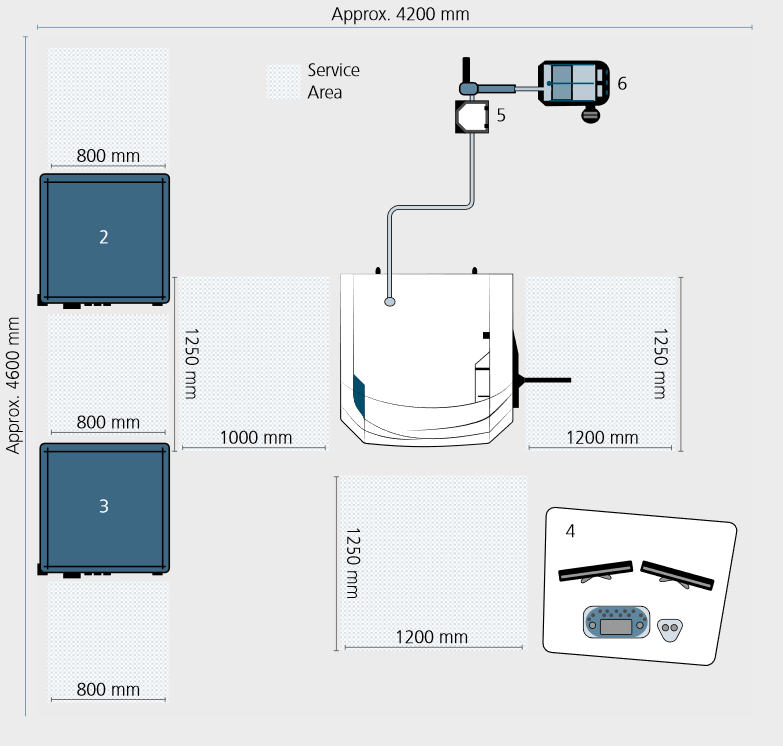
\includegraphics[width=0.6\textwidth]{SemFootprint.PNG}
		\caption[A schematic of The MultiSEMs space requirements]{\centering\label{SEMArea} A schematic of The MultiSEMs space requirements\cite{ZeissMulti}}

	
\end{figure}





We can now return to our earlier issue of filament replacement and other general maintenance; the MultiSEM 506 uses a Schottky Emitter (FEG) which has far the longest estimated lifetime however every machine is going to require at least 10 changes which we will estimate as delays of around 2 hours per machine per change. Extra maintenance such as recalibration of lenses and replacement of vacuum components can be included during the filament change and routine maintenance to other devices can occur in parallel. Therefore, we can calculate extra delays, assuming 10 trained engineers via:
\begin{align}
	Delays&= \frac{(Number\thinspace Of\thinspace Machines)\times (Maintenance \thinspace Time)}{ (Hours\thinspace In\thinspace a\thinspace year) \times (Number \thinspace of \thinspace Engineers) }\nonumber\\
	&= \frac{12,000\times20}{8760\times10}\nonumber\\
	&\approx 2.7\ Years
\end{align}

This delay seems rather large in comparison to our total imaging time however in reality machines will be maintained on a cycle, so that there is never any significant down time.

\subsection{Future and Feasibility}
\label{MultiSemMeth}
The consideration for imaging so far has been for one brain, with the hope of demonstrating the feasibility of the procedure. Once this has been achieved we believe that investment will be much easier to come by and we can increase our output rate significantly. Discussing the feasibility of the project with Dr. Anna Lena Eberle, Product Manager for ZEISS MultiSEM she commented:\\
\newline
"I think the main challenge is the amount of data that would be generated. I mean, there are humans orbiting earth, or projects like the Large Hadron Collider at CERN, or the fusion reactor ITER. With enough effort (=money and skilled people), I think the technical problems could be solved. When it comes to data storage or (even worse) handling or (even much worse!) processing, I am not so sure. But hopeful, nonetheless!"\\
\newline
 We'll begin to address some of the data issues in section 6 but this offers some hope that, provided significant funding, we can produce a fully automated pipeline for whole human brain imaging.\\
We also inquired as to the future of MultiBeam technology. Whilst ZEISS currently do not have plans to increase the number of beams in use, according to theoretical electron-optics, it would be possible to scale up to 331 beams provided enough funding and willing engineers. Any higher, and more research would have to be done, particularly concerning the performance of the electron source and again the data processes. The impact of an increase to 331 beams would be significant, assuming a proportional area increase, almost quartering our imaging time. It also appears plausible suggesting that, should we wish to acquire or produce these machines ourselves, we should be considering 331 beams as a target. \\

We wish to increase capacity in the future so that a brain can be processed in much reduced time, say for example 1 year. Currently that would require a 10 fold increase of the MultiSEM 506 machines and as we've already made clear, the difficulties of obtaining 12000 machines is one of the most significant tasks we will face. It may be necessary for us to acquire the rights to mass produce the MultiSEM technology as currently Zeiss would not have the capacity to support current numbers, yet alone the increase to 120,000 machines. The addition of a further manufacturing processes within our operation adds an entire new layer of complication, so for now we will assume this responsibility can be outsourced and that manufacturing cost will be equal to our quoted price. 
Fortunately what we do have on our side is time, as was stated in the section on expansion microscopy, new techniques are starting to invade the nanoscale microscopy market. This will hopefully provide us with additions to our pipeline rather than replacements, as that would be a significant loss on our initial investment. Furthermore Zeiss have stated that their product is extremely scalable, as we've seen with the transition from 61 to 91 beams and with the plausibility of 331. Therefore we can conclude that  using higher numbers of microscopes now would be a mistake, as new techniques may allow for much faster and cheaper imaging of the brain.\\


\subsection{Summary}

Below is a multi-criteria analysis (in tables \ref{RecSumP1} and \ref{RecSumP2}) to demonstrate the pros and cons of each considered method. It must be kept in mind that whilst all methods achieve a relatively close score, in reality there is a fixed cut off for resolution that discounts the majority immediately. Realistically we could have used a much higher weighting for resolution, however this would heavily skew the scoring hiding the merits of each method. As can be seen the MultiSEM comes out as the best method, as is to be expected. The small variance across scores suggests that new developments could at any point surpass the imagining capabilities of the MultiSEM. Whilst we must be vigilant in monitoring these, particularly in the area of expansion microscopy (once it has been shown to work with enough fluorescent labels STORM et. al. techniques) there is also a need commit to a currently available option in order to move forward. Startup costs are in most cases estimated from online retailers \footnote{http://www.labx.com/electron-microscope [Accessed 05/03/2016]} of similar equipment with the exception of the MultiSEM 506 price provided by Dr Eberle. Prospects are a representative figure of the likeliness a method will become a viable option or increase its capacity as a useful imaging tool for us in the future. Sample preparation includes the need for cutting as well as the staining and/or attachment of fluorescent dyes. 

\vspace{2cm}

\begin{table}[!htbp]
	\centering
	\caption{Summary of Considered Methods}
	\label{RecSumP1}
	\begin{tabular}{|l|l|l|l|l|l|l|l|}
		\hline
		\textbf{Part 1}       & \textbf{Weighting} & \textbf{\begin{tabular}[c]{@{}l@{}}MRI/ \\fMRI\end{tabular}} & \textbf{MRFM} & \textbf{\begin{tabular}[c]{@{}l@{}}LM  \\ (confocal)\end{tabular}} & \textbf{FM} & \textbf{STED} & \textbf{STORM} \\ \hline
		\textbf{Resolution}   & 5                  & 1                    & 5             & 1      & 1  & 1  &1 \\ \hline   
		\textbf{Startup cost} & 3                  & 4                    & 4             & 5      & 5  & 5  &5 \\ \hline
		\textbf{Speed}        & 3                  & 4                    & 2             & 5      & 5  & 4  &4 \\ \hline
		\textbf{Prospects}    & 3                  & 2                    & 2             & 1      & 2  & 4  &4 \\ \hline
		\textbf{Sample Prep}  & 3                  & 4                    & 1             & 5      & 3  & 3  &3 \\ \hline
		\textbf{Score}        &                    & 47                   & 52            & 53     & 50 & 53 &53 \\ \hline
	\end{tabular}
\end{table}

\clearpage

%%%%%%

\begin{table}[!htbp]
	\centering
	\caption{Summary of Considered Methods}
	\label{RecSumP2}
	\begin{tabular}{|l|l|l|l|l|l|l|}
		\hline
		\textbf{Part 2}       & \textbf{Weighting} & \textbf{\begin{tabular}[c]{@{}l@{}}ExM\\ (with FM)\end{tabular}} & \textbf{XRay} & \textbf{TEM} & \textbf{SEM} & \textbf{MultiSEM} \\ \hline
		\textbf{Resolution}   & 5                                                        & 1  & 5  & 5  & 5  & 5           \\ \hline
		\textbf{Startup cost} & 3                                                          & 4  & 3  & 2  & 3  & 1           \\ \hline
		\textbf{Speed}        & 3                                                         & 4  & 2  & 2  & 2  & 3           \\ \hline
		\textbf{Prospects}    & 3                                                        & 5  & 2  & 3  & 2  & 4           \\ \hline
		\textbf{Sample Prep}  & 3                                                        & 3  & 2  & 2  & 2  & 2           \\ \hline
		\textbf{Score}        &                                                          & 53 &  52 & 52 & 52 & \textbf{55} \\ \hline
	\end{tabular}
\end{table}


Finally a short overview of the chosen microscopes major features which will be used later in our section on costings (Section \ref{Business_Case}) is provided in table \ref{MultiSEMSum}.


\begin{table}[!htpb]
	\centering
	\caption{MultiSEM 506 Summary}
	\label{MultiSEMSum}
	\begin{tabular}{|l|l|}
		\hline
		\textbf{Resolution} & 4 nm   \\ \hline
		\textbf{Power Consumption} & 4kW   \\ \hline
		\textbf{Cost per machine} & ~\pounds 3 Million \\ \hline
		\textbf{Initial amount of machines} & 12000   \\ \hline
		\textbf{Area per machine} & 16.8 m$^{2}$  \\ \hline
	\end{tabular}
\end{table}

	
	%Wojciech's stuff
		\newpage
		
		\clearpage
			
		\pagestyle{wojciech}
		
		\section{Data organisation and querying}
		
		\subsection{Data organisation}
		The novel EM imaging techniques described above made it possible to discern the most minute neuronal structures. This impressive resolution comes at a cost, though, which is the explosion of storage space required for the brain data. The storage space required for only a single cortical column (as stated by Kleissas et al. \cite{kleissaslarge}) is \textbf{1 petabyte}. Clearly, the supposed storage of the whole human brain's pictorial representation does not scale to reasonable values under the current techniques. A reliable and widespread approach is to convert the images into textual files containing only the most compelling information. This is widely used in web development (HTML, CSS) or describing biochemical network interactions (SBML, \cite{hucka2003systems}) and attempts have been made to develop similar frameworks in the field of connectomics, most notably NeuroML \cite{gleeson2010neuroml}  and CAJAL3D \cite{kleissaslarge}.
		
		\subsubsection{NeuroML}
		
		Based on XML (eXtensible Markup Language), NeuroML is a robust framework allowing for a lightweight representation of a variety of neuronal data. It builds on several layers of biological complexity and offers an exhaustive model for storing a wiring diagram of the human brain. \\
		It comprises of \textbf{three basic levels}:
		\begin{enumerate}
			\item The \textbf{first} level defines the neuronal morphologies of the elemental cells and metadata (additional information about model components). The segments (basic representation units, e.g. dendrites of axons) are described using their geometrical properties and the ancestor ID (parent segment). Metadata can comprise of the model authors or other references.
			\item The \textbf{second} level is centred around the electrical properties of the neuronal tissue. It provides a way of describing several different conductance types as well as extended morphological features such as the synaptic plasticity (able to reproduce behaviours such as Hebbian and anti-Hebbian learning) or channel densities of various parts of the cells.
			\item The third level is the most relevant to our application. It describes the neural networks in terms of their anatomical structures and synaptic connectivity (listing \ref{lst:neuroml}). It serves as both an explicit descriptor of the cell positions and \textbf{synaptic connectivity}, or an algorithmic descriptor of the desired neuronal pattern generation.
		\end{enumerate}
		
		
		\begin{lstlisting}[caption={A population object in NeuroML},label={lst:neuroml}]
		<population name="CellGroupB" cell_type="CellA">
		<instances size="2">
		<instance id="0"><location x="0" y="100" z="0"/></instance>
		<instance id="1"><location x="20" y="100" z="0"/></instance>
		</instances>
		</population>
		\end{lstlisting}
		
		\subsubsection{CAJAL3D}
		\label{Cajal}
		\textbf{C}onnectome \textbf{A}nnotation through \textbf{J}oint \textbf{A}nalysis of \textbf{L}arge \textbf{3}-dimensional \textbf{D}ata is an initiative developed by the scientists from Johns Jopkins University. It is used in conjunction with the Open Connectome project, and as such it offers a comprehensive set of annotation and programmatic tools, such as:
		
		\begin{enumerate}
			\item \textbf{R}eusable \textbf{A}nnotation \textbf{M}arkup for \textbf{O}pen co\textbf{N}nectomes (RAMON) standardizes the annotations and descriptions of the neuronal structures (listing \ref{lst:ramon}). It is compatible with various algorithms and standards used by multiple institutions.
			RAMON supports the descriptions of objects such as synapses, seeds, neurons, organelles, etc. \cite{burns2013open}
			
			\item Web services facilitating querying the neuronal object database combined with MATLAB Application Programming Interfaces as well as automated data analysis pipelines.
		\end{enumerate}
		
		\noindent The primary RAMON objects \cite{kasthuri2015github} are:
		\begin{itemize}
			\item RAMONSegment: individual neurites
			\item RAMONNeuron: container of RAMONSegments
			\item RAMONSynapse: neuronal connections
			\item RAMONOrganelle: sub-cellular objects
		\end{itemize}
		
		\subsubsection{Summary and design choice}
		
		\noindent As described in Gleeson et al., 2010 \cite{gleeson2010neuroml}, \textbf{NeuroML} is an ideal tool for description and annotation of neural tissue, even the highly biologically complex structures. Its main \textbf{advantages} include the easiness of transformation and rendering into some of the more popular visual and textual formats or scalability and modularity, which make it worth considering for our application. \\
		On the \textbf{downside}, due to the high level of detail it adheres to, it might be too specific, and thus too data-heavy, to store the whole brain's neuronal data. Given the scale of the project, the compressibility of the stored data is a crucial factor. \\
		
		\noindent On the other hand, CAJAL3D is a \textbf{lightweight} framework containing a set of minimum
		annotation data necessary for capturing the biological information. It is ideal for our application, due to its ability to compress large neuronal datasets into manageable sizes. In addition, it is widely used within the Open Connectome project community, which guarantees its continued development and support. It comes with a range of APIs and data processing frameworks. After the mentioned considerations, we decided to \textbf{use CAJAL3D} as our data organisation framework.
		
		\begin{lstlisting}[caption={Creating a RAMON object},label={lst:ramon}]
		cube = RAMONVolume;
		cube.setResolution(1);
		cube.setCutout(d);
		cube.setChannel(channel);
		cube.setChannelType(eRAMONChannelType.annotation);
		cube.setDataType(eRAMONChannelDataType.uint32);
		cube.setXyzOffset([xstart, ystart, zstart]);
		protoRAMON = 'RAMONSynapse()';
		useSemaphore = 0;
		\end{lstlisting}
		
		\subsection{Data querying}
		Even though not imperative in our application, possessing an appropriate set of tools for querying the data is still worth mentioning. There exists a range of such programs developed independently by several research groups. The most relevant are listed below.
		
		\subsubsection{WaferMapper}
		Designed specifically for the use with Automated Tape-Collecting Ultra-Microtome (ATUM), it is a reliable and widely compatible tool for EM neuronal image handling. It is ideal for mapping, alig nment and annotation of the scans, and offers some library querying algorithms. \cite{hayworth2014atum}
		
		\subsubsection{TrakEM2}
		TrakEM2 \cite{cardona2012trakem2} extends the functionality of WaferMapper in its rapid and efficient access to the image database. Its simplified GUI facilitates Manipulating, visualizing, reconstructing, annotating and measuring neural components. Identification and labelling of neurons and synapses in the image volume is furthermore heavily computer-assisted in order to minimise the chance of a human error.
		
		\subsubsection{ConnectomeExplorer}
		
		Given that the tools above focus rather on the \textbf{local} manipulation and visualisation of the neural images, there exists a need for more powerful, global query software. This was the motivation behind the development of ConnectomeExplorer \cite{beyer2013connectomeexplorer}, which is built on three complementary layers:
		\begin{itemize}
			\item The first one offers functionality within which the previous two could operate (one similar to WaferMapper and TrakEM2) i.e. handling and visualisation of large volumes of 3D image sets.
			
			\item Perhaps the most important one is the novel implementation of query (set) algebra which allows for efficient spatial and connectivity/topological interrogation of the segmented dataset (listing  \ref{lst:connectomeexplorer}). This allows for a robust statistical analysis of the annotated tissue.
			
			\item The third layer supports the first two with an intuitive user interface for viewing the results of statistical queries. It is optimised to handle multiple views and concurrent analysis of multiple image regions.
		\end{itemize}
		
		\begin{lstlisting}[caption={An example of a query in ConnectomeExplorer},label={lst:connectomeexplorer}]
		// What is the average number of vesicles over all axons, and what is the average number of vesicles of each axon?
		// returns a set of tuples for all axons and their synapses
		2a := <axons,synapses>
		2b := [avg(vesicleCount)]<2a> // avg over all axons
		2c := [group(1)]<2a> // set of sets, grouped by axon
		2d := [avg(vesicleCount)]<2c> // avg for each axon
		\end{lstlisting}
		
		\subsubsection{Summary and design choice}
		
		\noindent It is clear that the tree tools described above (WaferMapper, TrakEM2 and ConnectomeExplorer) serve distinct purposes and can (or should) be used at different stages of the process: WaferMapper at the very beginning, TrakEM2 before and during segmentation and ConnectomeExplorer after identifying the neural components within the tissue. They will most definitely enhance the process efficiency and increase the subsequent understanding of the collected data. Since all three are open-source, academically developed software packages, \textbf{we can benefit from using all of them} without having to commit to any particular one, provided our data formats are compliant with the software requirements.
		
		\section{Data storage}
		\label{data_storage}
		As mentioned before, given the resolution of the electron microscope scans of the brain, it comes as no surprise that their storage exceeds any reasonable, viable magnitudes. Scaling the 12 terabyte for $450 \times 350 \times 50 \mu m^3$ region of mouse visual cortex \cite{kleissaslarge} to the human brain's volume of around $1400 cm^3$ gives:
		\begin{equation}
		\textrm{storage requirement} = \frac{1400 \times (10^{-2})^3}{450\times 350 \times 50 \times (10^{-6})^3} \times 12 \textrm{TB} = 2.133 \times 10^6 \textrm{PB}
		\end{equation}
		That's about \textbf{double the predicted internet traffic} in 2016 \cite{telegraph2016traffic} and significantly more than could ever be reasonably stored using the existing technology. The aforementioned storage and compression techniques, though, give a more optimistic outlook on the problem. The Open Connectome project website contains some annotated data for a region known as AC4 - adult olfactory receptor neuron of a drosophila fly. The segmentation data i.e. the refined connectomic model accounts for about $1.486 \textrm{MB}$ of storage identifying a $1024px\times1024px\times100layers$ tif image stack. This is conveniently stored in the RAMON data format that is also our framework of choice. In physical terms, this corresponds to a neural region of approximately $1024\times1024\times100\times29^3 nm^3=2557.4\mu m ^3$. Hence the storage requirement for the whole human brain would be:
		\begin{equation}
		\textrm{storage requirement} = \frac{1400 \times (10^{-2})^3}{2557.4\times  \times (10^{-6})^3} \times 1.486 \textrm{MB} = 757.6 \textrm{PB}
		\end{equation}
		This is clearly a lot more manageable. Having a value to play with, we can now investigate the possible storage methods, their access time and associated cost.\\
		
		\noindent \textbf{Local storage} is one of the options, as it provides a simple and seemingly quick access to data. As used in the Burns et al. 2014 paper \cite{burns2013open}, an OCZ Vertex 4 drive is capable of storing up to 512GB with roughly 500MB/s read and write speeds. For one human brain, we would therefore require around \textbf{1.5 million} of such drives, with the idealised access time of \textbf{48 years} (!), not even taking into account the access non-idealities and redundancy. The cost of such an SSD - about \pounds100, blows the cost of the project to about \textbf{\pounds150 million} for storage alone.\\
		
		\noindent \textbf{Cloud storage} solutions became extremely popular in the last years, due to the increased internet bandwidth allowing for high read and write speeds as well as the online storage space getting cheaper. One of the current leading providers of the cloud storage solutions is Amazon AWS, who provides Amazon Glacier service for long-term backup. The cost is around \pounds0.005 per gigabyte per month, amounting to around \textbf{\pounds190 million} for ten year storage. \\
		
		\subsubsection{Summary, design choice and future outlooks}
		
		\noindent The \textbf{SSD storage} is a \textbf{traditionally tested and trustworthy} solution. The data access speeds, however slow, do not have a great impact on the project's success, especially given inferior figures of the alternative.	\textbf{The downsides} include the need for maintenance and storage of the drives, that would be otherwise handed over to external companies. \\
		
		\noindent The \textbf{advantages of cloud storage} involve mainly the easiness of use - the maintenance and safety of the server space is included in the price and guaranteed by the provider. \textbf{On the other hand}, given the long time-scale of the project we should expect the cloud solution's cost to significantly surpass the alternative one. Moreover, the success of an online storage solution would depend largely on a good internet connection, which would adversely affect the financial aspect of the project. \\
		
		\noindent All factors considered, we decided to \textbf{use the local SSD storage} for the project. This is not a definite commitment, though, and as the cloud technology matures, hybrid solutions may be taken into account. \\
		
		\noindent All the considerations have assumed a noteworthy simplification: storing only RAMON annotated data. This is possible only if the data is transformed into such a form straight after recording, or at least with a buffer large enough to temporarily store the data before it can be segmented. No matter how quickly we manage to store or access the data, the segmentation is still the temporal bottleneck of the process. \\
		
		\noindent At this point it is also useful to mention that there is research underway concerning novel storage methods such as 5D Ultrafast Laser Nanostructuring in Glass \cite{zhang20135d}. It is an optical storage method based on a femtosecond laser writing in the bulk of transparent material, which allows for stunning parameters such as 360TB/disc data capacity, 1000\degree C thermal stability and practically unlimited lifetime. That would limit the number of storage discs to about 2000, yet the cost or time of market introduction of the method is not known.
		
		\section{Segmentation}
		\label{segmentation}
		\subsection{Manual segmentation}
		With the human brain containing hundreds of billions of neurons and hundreds of trillions synaptic connections, it seems clear that the task of segmenting the EM images of the neural tissue is the most ambitious one along our pipeline. Not only is the process hard, given that accurate synapse recognition requires experience in the neuroscience area, but also significantly time-consuming. As stated by Kasthuri et al., 2015 \cite{kasthuri2015saturated}, manual segmentation of the whole human brain would require about $ 2 \times 10^{15}$ human years, assuming continuous, 24/7 work, or $3.2 \times 10^{10}$ human years, extrapolating from the figure in \cite{mishchenko2009automation}. Clearly, this is not in any case viable, but doesn't fully rule out the method. The automatic segmentation algorithms, described later, use machine learning techniques to interpret the neuronal tissue images. The learning part of the process relies on supplying the algorithm with appropriate training data, based on which it can differentiate between synaptic and non synaptic regions. Such data can only be produced manually, but certainly in smaller volumes. \\
		A useful tool for the manual segmentation has been developed by the team of researchers contributing to the open connectome project. VAST (\textbf{V}olume \textbf{A}nnotation and \textbf{S}egmentation \textbf{T}ool) allows for computer-assisted manual processing of the images in order to find the regions of interest (see fig \ref{fig:manual_segmentation}). Given that the tool is open-source, well-documented and continually supported, it will fit well within our image-processing pipeline. It is worth mentioning that using VAST yielded over 99\% accuracy of the segmentation, with the further inconsistencies later corrected by joint tracing of two experienced researchers.
		
		\begin{figure}
			\centering
			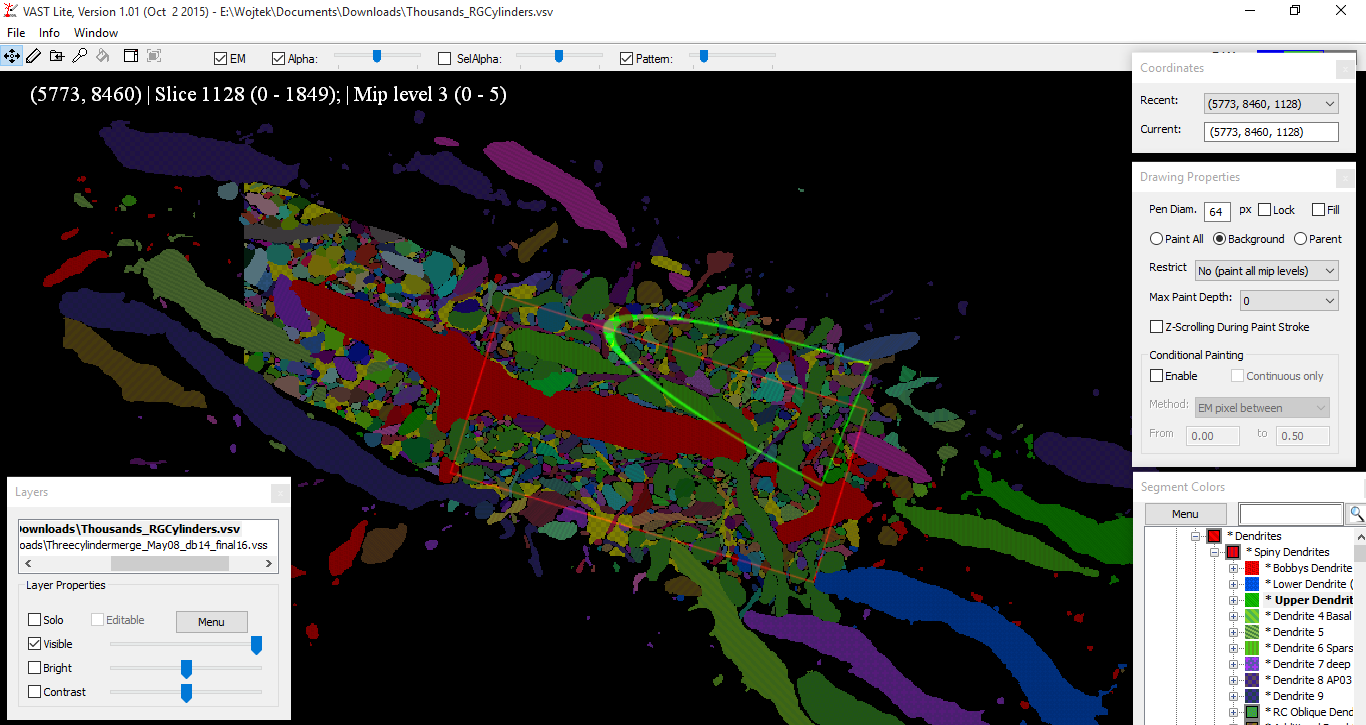
\includegraphics[width=0.70\textwidth]{manual_segmentation.PNG}
			\caption{\label{fig:manual_segmentation}Caption from VAST - segmented neural cylinder}
		\end{figure}
		
		\subsection{Machine learning}
		\label{MachLearn}
		Once we have collected the training data using the manual segmentation methods described above we can start thinking about teaching the algorithms to do the segmentation for us. Algorithmic identification of the synapses and other neuronal structures offers a clear advantage over the accurate, but labour-intensive manual segmentation process - time. Attempts have been made before by several different research groups to automatically segment the neural tissue images:
		
		\begin{itemize}
			\item RhoANA, developed in conjunction with VAST largely by the team of researchers at Harvard contributing to the Open Connectome project (Kasthuri et al., 2015 \cite{kasthuri2015saturated}). It is based on deep-learning convolutional neural networks (described in length in the later sections) and GALA (Graph-based active learning of agglomeration). The accuracy achieved was 92.6\% (pixel classification) or 87.6\% (profile classification). Nevertheless, the outcome still needed human assistance for effective segmentation.
			
			\item A paper by Jain et al. (2010, \cite{jain2010machines}) presents various methods for image pre-processing and segmentation quality scoring, but concludes with a note on possible usefulness of the convolutional neural nets used above.
			
			\item An alternative approach has been presented in the paper by Mishchenko, Y., 2009 \cite{mishchenko2009automation}. It emphasises the need for heavy \textbf{pre-processing} of the images (as opposed to letting the convolutional layers do it for us), with the use of neural nets for later parts of the process. The method penalized merge errors more than over-segmentation, achieving 2.5/1000 and 50/100 misclassification respectively. With a significant help of human tracers, the method achieved a reconstruction error rate of 0.2-0.4\%, using significant man-hour input, though. 
		\end{itemize}
		
		\noindent The algorithms described above proved to be an extremely useful learning material while working to develop our own automatic segmentation pipeline. Three main techniques have been considered while choosing an appropriate method for the task at hand, all described below.
		
		\subsubsection{Segmentation scoring}
		At this point it is worth quickly mentioning how the segmentation results are scored. After the tiff stack is produced, it can be contrasted against the ground truth using a measure called the F1 score. It takes into account four kinds of matching between the prediction (P) and ground truth (GT): True Positive (P true when GT true), False Positive (P false when GT true), True Negative (P true when GT false) and False Negative (P false when GT false). We'd like to maximise the number of True Positives and False Negatives, hence the F1 penalises the other two, by using the following calculation:
		\begin{align}
		F1 = \frac{2\times TP}{2\times TP + FN + FP}
		\end{align}
		which is easily interpretable as it lies between 0 and 1.
		
		\subsubsection{Logistic regression}
		The problem of image segmentation, and in fact most machine learning problems, has at its core the pursuit for a function appropriately fitting or classifying a dataset. In a simple 2D case this might just be fitting a particular function to a couple of points in order to minimize some cost, e.g. the least squares error. In more advanced cases we are trying to separate distinctly labelled, multidimensional datasets using a decision boundary i.e. learn a conditional distribution of the class label given the input.
		
		\noindent Usually, we are given data points possessing certain features i.e. coordinates in the multidimensional space, and their class, e.g. 0 or 1, blue or red, synapse or non-synapse. Assuming we can segment the set based on the supplied coordinates, we can also try to guess the importance of the features and predict a point's class depending on its coordinates. In logistic regression, we use a function called the logistic sigmoid in order to define the null hypothesis $h_0$ (fig. \ref{fig:logistic_regression}). It is given by:
		\begin{equation}
		\sigma (x_i ^T \beta) = \frac{1}{1+exp(-x_i ^T \beta)}
		\end{equation}
		where $x_i$ is the feature vector and appropriate entries in $\beta$ are the feature weights whose values we are trying to optimize in order segment the data correctly. We can interpret the logistic sigmoid as the probability that y=1 on an input x. Using this, we can use a noise distribution that penalises misclassification. One such distribution is a simple Bernoulli:
		\begin{equation}
		p(y_i | ...) = \sigma ^ {y_i} (1-\sigma) ^ {1-y_i}
		\end{equation}
		
		\begin{figure}
			\centering
			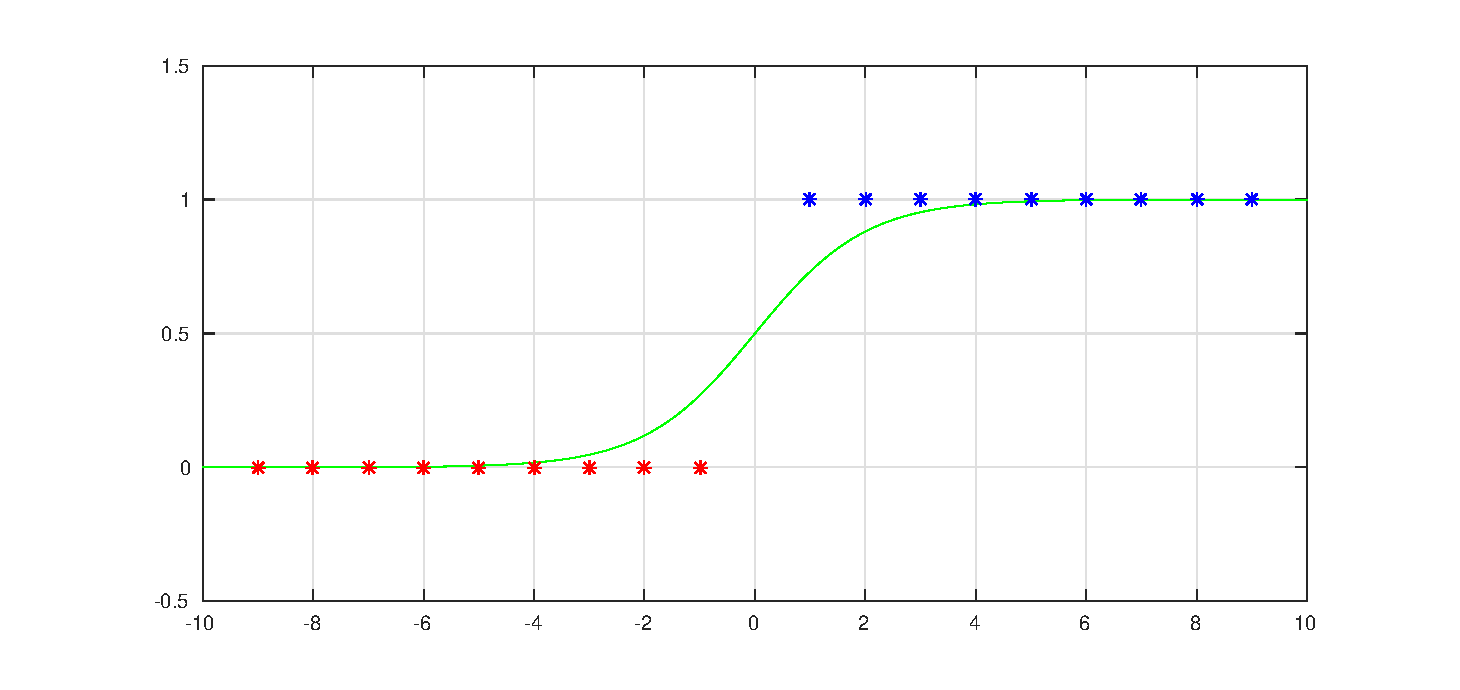
\includegraphics[width=0.70\textwidth]{logistic_regression.eps}
			\caption{\label{fig:logistic_regression}{Logistic sigmoid function}}
		\end{figure}
		
		\noindent where $y_i$ is the observed output. Now we can train the classifier to maximize the likelihood of a particular value of $y_i$ occuring given the feature vector $x_i$. Taking logs and differentiating we get:
		\begin{equation}
		\frac{\partial}{\partial \beta} log(\mathcal{L}) = \frac{\partial}{\partial \beta} log (\prod_{i}^{} p(y_i | ...) ) = \frac{\partial}{\partial \beta} log (\prod_{i}^{} \sigma ^ {y_i} (1-\sigma) ^ {1-y_i}) = 0
		\end{equation}
		
		\noindent This can be computed numerically using methods such as gradient descent in order to find the feature weights in $\beta$.\\
		Logistic regression is a hugely useful, powerful and relatively simple tool. It makes sure that data is not overfitted and provides a useful starting point for the investigation. Due to its nature, though, it deals well only with linear models, or at least ones that are easily linearised.
		
		\subsubsection{Random forests}
		Random forests provide another method for classifying a dataset based on a set of features. Their most basic and most important component is a decision tree.\\
		
		\noindent A \textbf{decision tree} is a tree-like structure that classifies a member of some dataset based on its features. The leaves of such tree always lead to a discrete class decision, in our case 0 or 1 based on whether a component is a synapse or not. The nodes within the tree are binary classifiers that lead into one of their children depending on a particular feature value (see fig. \ref{fig:decision_tree}). As described in length later, our classification is based on around 10 distinct features of image components that have been identified as synapse candidates.\\
		
		\noindent Training a single decision tree to classify the data is often impractical, as it leads to overfitting. The learning process focuses on conforming to the training dataset, hence compromising accuracy of fitting to the validation set. Several techniques have been developed to mitigate this, with the most prominent ones being \textbf{boosting} and \textbf{bagging}. They aim to provide a more accurate classification thanks to using multiple decision trees, or as a matter of fact any learners such as neural nets.
		
		\begin{figure}[!h]
			\centering
			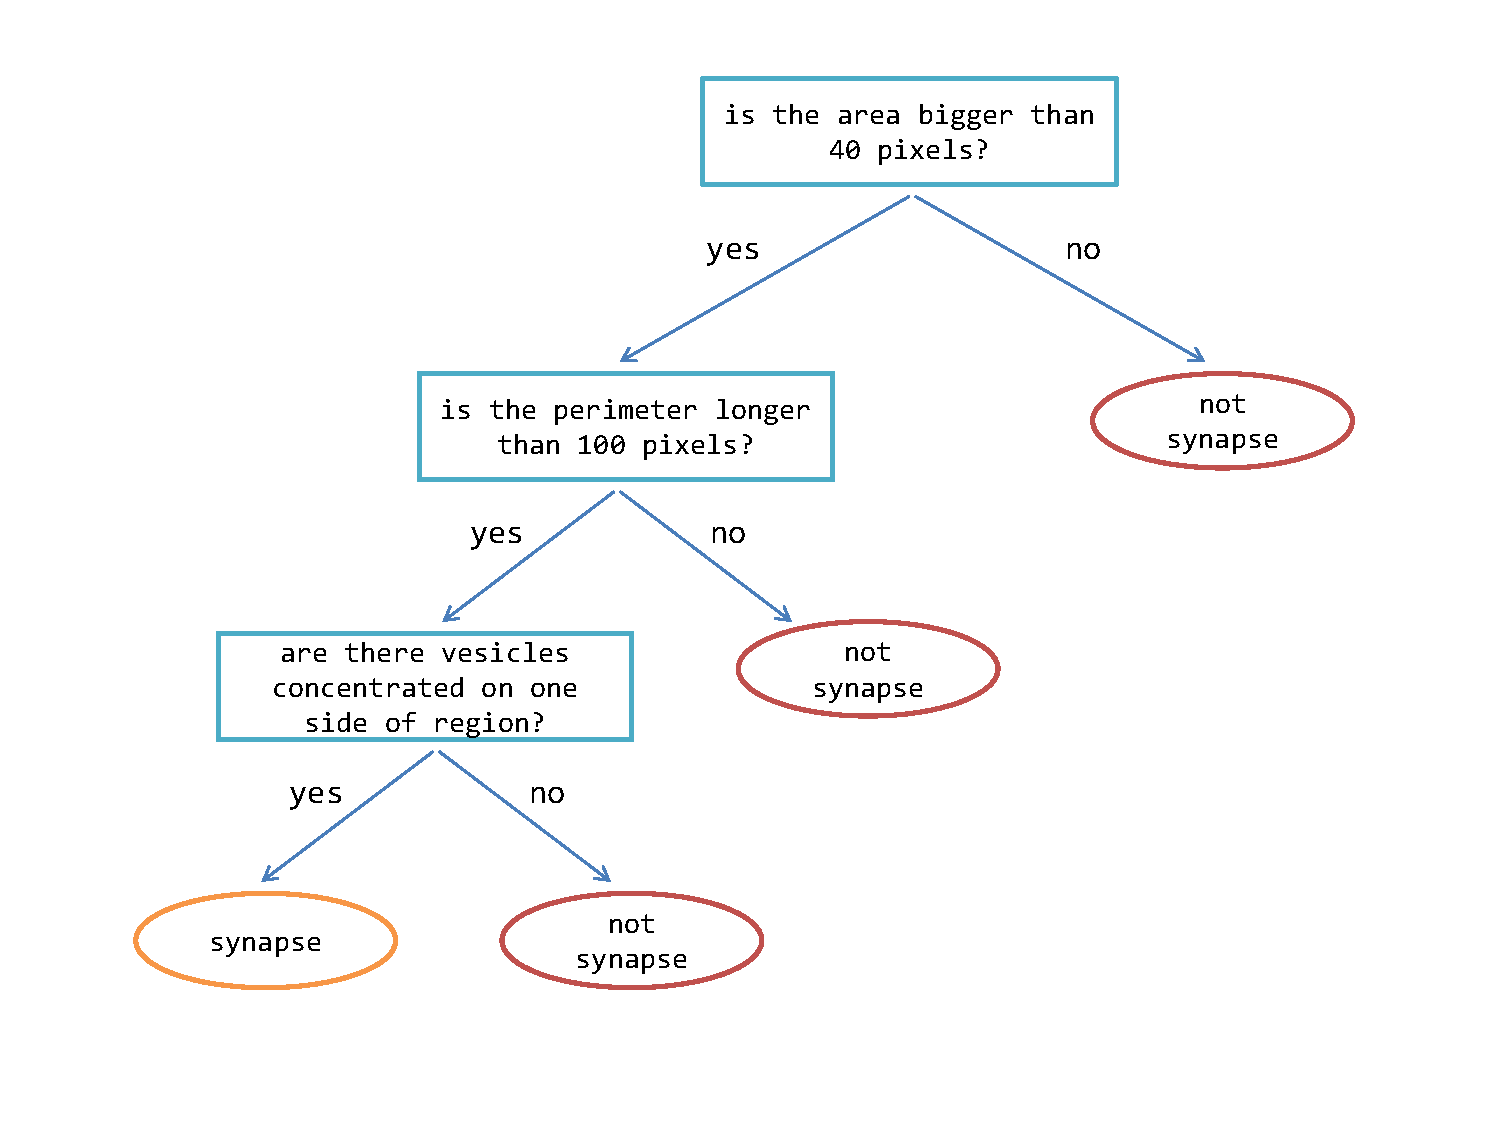
\includegraphics[page=1,width=0.60\textwidth]{decision_tree.pdf}
			\caption{\label{fig:decision_tree}{An extremely simplified example of a decision tree}}
		\end{figure}
		
		\noindent Before we go into describing boosting and bagging, it is worth defining a \textbf{weak learner}. Since we usually deal with large datasets, we can safely assume that by sampling the set we can obtain a subset to some extent statistically representative of the whole population. Based on that subset, we can train a classifier that is not necessarily well-correlated with the whole dataset, but whose output is at least better than random guessing. In theory, by combining several of those weak (or base) learners, we can derive a classifier capable of obtaining labelling closer to the ground truth.  The base learners used need not to be decision forests, they may well be logistic regression classifiers, neural nets, or others.\\
		
		\noindent \textbf{Boosting} \cite{bishop2006pattern} is a sequential learning algorithm that trains the weak learners one after another. The classifiers are supplied with the weighted dataset that was computed in previous stages. Given that weak learners provide classification in theory better than random, each subsequent stage should come up with an answer closer to the ground truth. This is enhanced by penalising misclassification i.e. giving greater importance to points that were incorrectly classified by previous learners. After the classifiers are trained, we can combine their output through a weighted majority voting scheme. This strategy is known as the AdaBoost algorithm.\\
		
		\noindent \textbf{Bagging} \cite{murphy2012machine} or "bootstrap aggregating" approaches the learning from a frequentist perspective i.e. given that we train enough weak learners, we can combine their (individually faulty) outputs to provide the correct classification. A refined version of the bagging algorithm, i.e. the random forest, uses randomly chosen subsets of data in order to train base classifiers later combined to provide a correct classification. \\
		
		\noindent MATLAB's function TreeBagger \cite{matlab2015treebagger} creates an ensemble of bagged decision trees. Provided with an input matrix (where rows are data points and columns are their corresponding features) and an output vector (row labels - synapse/non-synapse), the function tries to train a specified number of decision trees as an ensemble. These are later used to compute the response using the weighted average of the tree predictions i.e.:
		\begin{equation}
		\hat{y} = \dfrac{1}{\sum_{t=1}^{T} a_t I(t \in S)} \sum_{t=1}^{T} \alpha_t \hat{P}_t(c|x)I(t\in S)
		\end{equation}
		where $\hat{y}_t$ is the prediction from tree $t$ in the ensemble, $S$ is the set of indices of selected trees that comprise the prediction, $I(t\in S)$ is 1 if t in the set S, and 0 otherwise and $\alpha_t$ is the weight of tree $t$.\\
		Using TreeBagger on our dataset using the regional classification methods described later yielded F1 score of about $12.5\%$. This will later be contrasted with the neural net performance. \\
		
		\noindent Random forests are an accurate and easy to use classification method. Even though largely more versatile than logistic regression, random forests are not an answer to all kinds of problems. If we wish to train too many individual learners to make up the final ensemble, the algorithm may become too slow, as instead of learning it will just try to memorize the dataset. Having found a baseline for further investigation, we decided to try to segment the set with neural nets, described below.
		
		\subsubsection{Artificial neural networks}
		\cite{ng2015coursera} It was noted at the end of the logistic regression section above that its most obvious drawback is the inability to cope with non-linear datasets. This is largely due to the fact that expanding the feature set to include the non-linearities (e.g. quadratic cross feature products) would grow the storage space unreasonably. Both random forests and artificial neural networks are in theory able to address that problem. Their inherently non-linear architectures help conforming to more diverse and complex classification challenges. \\
		
		\noindent As the name suggests, the artificial neural networks are loosely based on the human brain's intricate internal architecture. Their most basic building block is a logistic unit, which works similarly to a logistic regression classifier.
		
		\begin{figure}[!h]
			\centering
			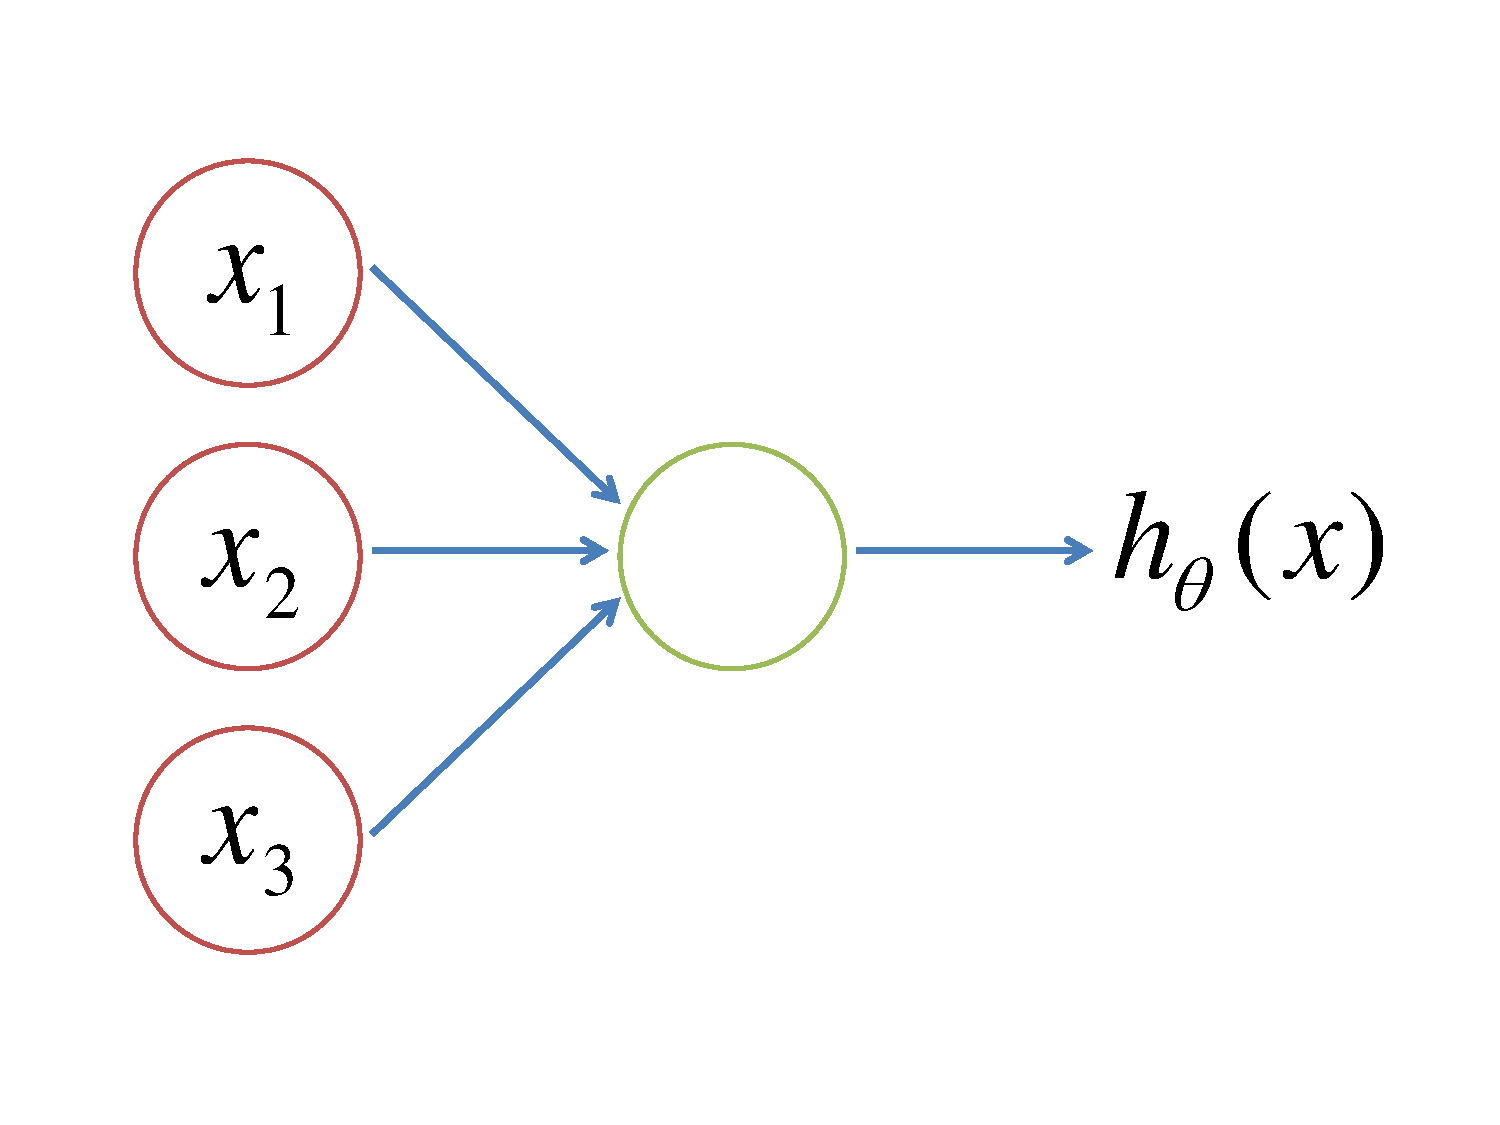
\includegraphics[page=1,width=0.40\textwidth]{logistic_unit.pdf}
			\caption{\label{fig:logistic_unit}{A logistic unit}}
		\end{figure}
		
		\noindent The logistic unit takes in input features $x_1, x_2, ..., x_n$ and makes an output decision using a logistic sigmoid function, i.e. (as before):
		
		\begin{equation}
		h_\theta (x) = \frac{1}{1+e^{-\theta ^ T x}}
		\end{equation}
		\noindent where $\theta$ are the feature weights.\\
		
		\noindent Naturally, many more of those logistic units are combined within a layer of a neural net and many more layers are combined to form a neural network (see fig. \ref{fig:neural_net}). It comprises of one input and one output layer, in addition to several (in case of the aforementioned figure just one) hidden layers. Output is then calculated according to:
		
		\begin{align}
		a_1^{(2)} &= \sigma (\Theta_{10}^{(1)} x_0 + \Theta_{11}^{(1)} x_1  + \Theta_{12}^{(1)} x_2  + \Theta_{13}^{(1)} x_3) \\
		a_2^{(2)} &= \sigma (\Theta_{20}^{(1)} x_0 + \Theta_{21}^{(1)} x_1  + \Theta_{22}^{(1)} x_2  + \Theta_{23}^{(1)} x_3) \\
		a_3^{(2)} &= \sigma (\Theta_{30}^{(1)} x_0 + \Theta_{31}^{(1)} x_1  + \Theta_{32}^{(1)} x_2  + \Theta_{33}^{(1)} x_3) \\
		\Rightarrow h_{\Theta} (x) &= \sigma (\Theta_{10}^{(2)} \boldsymbol{a_0} + \Theta_{11}^{(2)} \boldsymbol{a_1}  + \Theta_{12}^{(2)} \boldsymbol{a_2}  + \Theta_{13}^{(2)} \boldsymbol{a_3})
		\end{align}
		where the superscript denotes the layer number. Or, more compactly:
		\begin{align}
		a^{(2)} = \sigma(\Theta^{(1)} x^{(1)}) \\
		h_{\Theta}(x) = \sigma(\Theta^{(2)} a^{(2)})
		\end{align}
		
		\begin{figure}[!h]
			\centering
			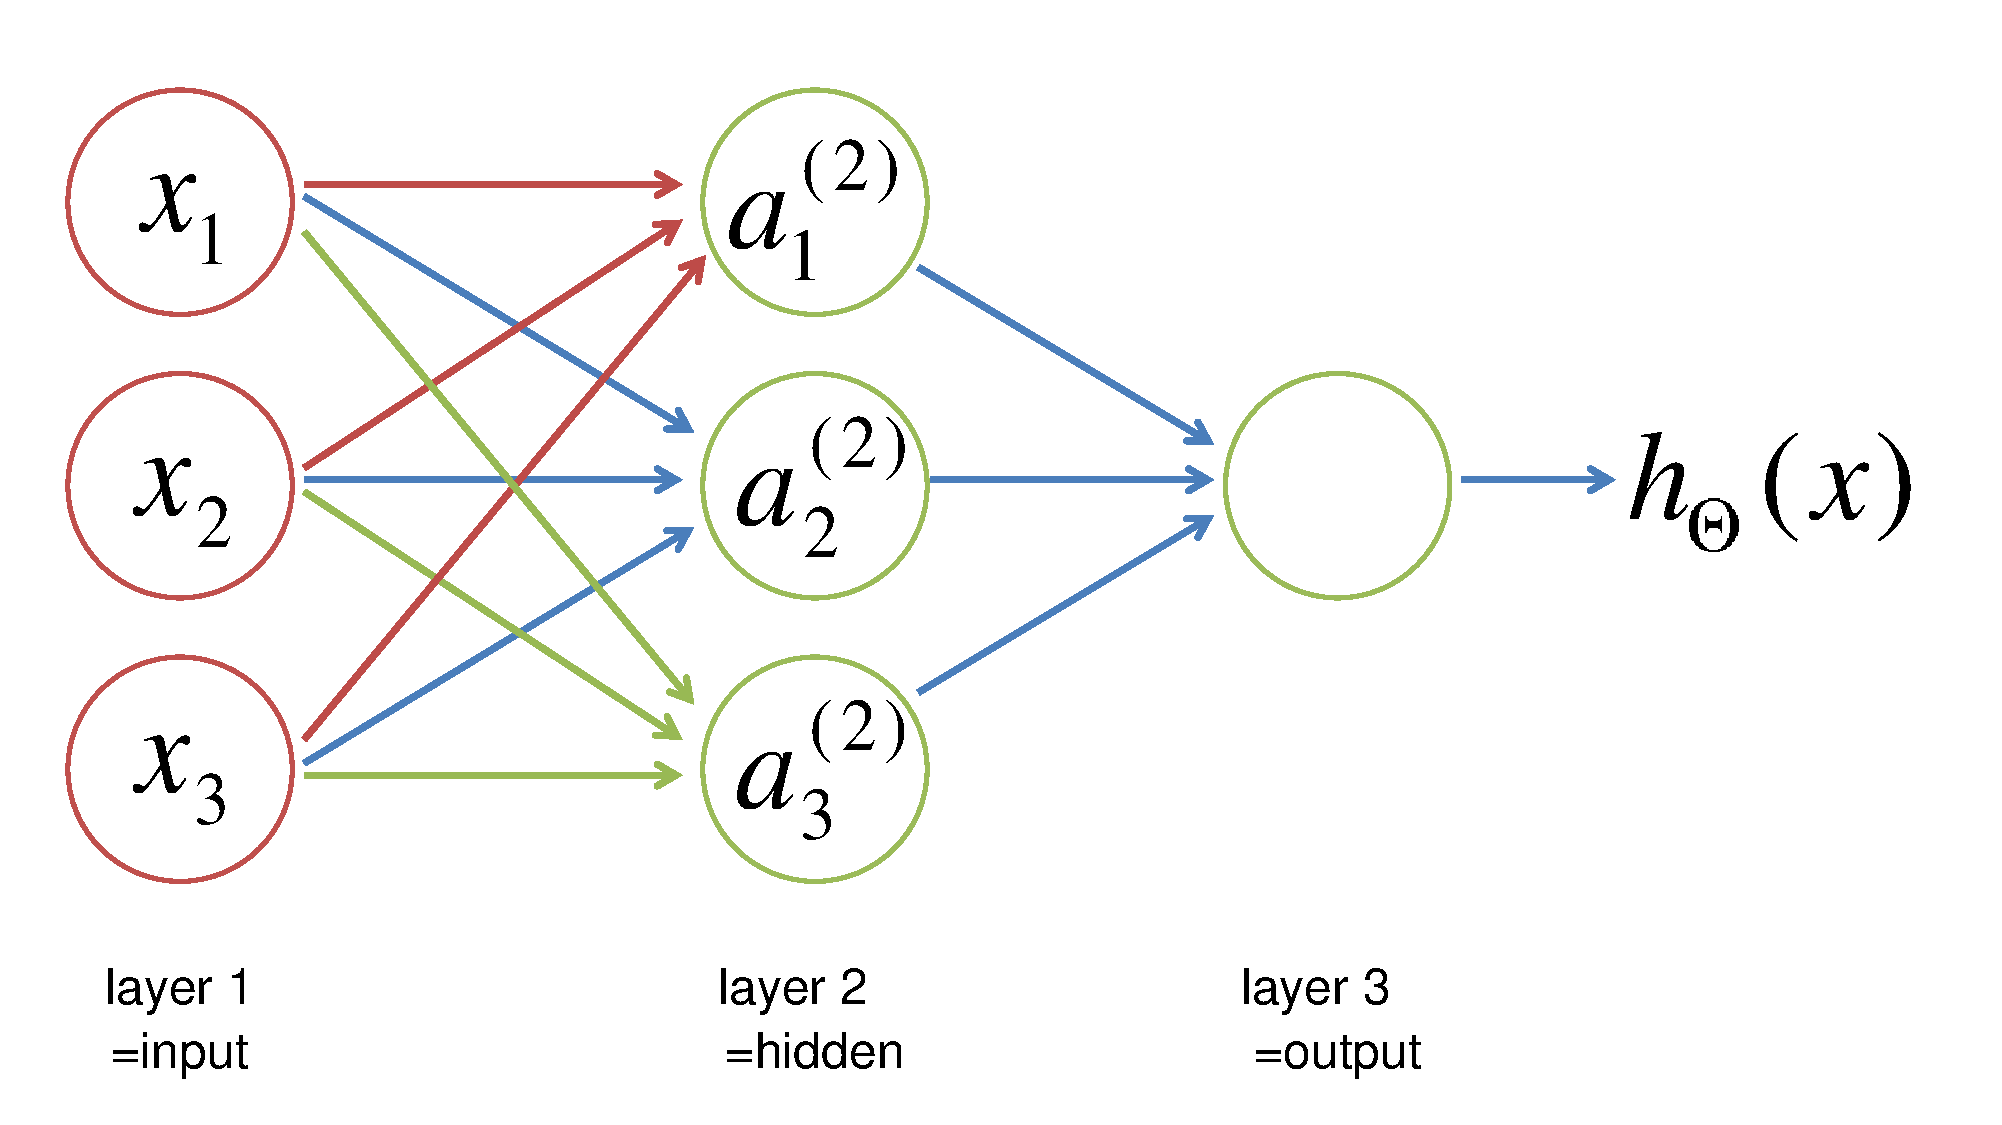
\includegraphics[page=1,width=0.60\textwidth]{neural_net.pdf}
			\caption{\label{fig:neural_net}{A simple neural net}}
		\end{figure}
		
		\noindent The computation above is called forward propagation, because it sequentially calculates the $a$ results for particular layers of logistic units using the previous ones. Now the most important feature of the neural nets is that the features within the layers (e.g. $a_1^{(2)}, a_2^{(2)}, a_3^{(2)}$) are "learnt" automatically, by appropriately tweaking the $\Theta$ vector using an algorithm called the back propagation.
		
		\noindent At the heart of many learning algorithms is minimisation of some kind of a cost function. Neural networks are one such algorithm, where the cost function is defined as:
		\begin{equation}
		J(\Theta) = - \frac{1}{m} \Bigg[\sum_{i=1}^{m} \sum_{k=1}^{K} y_k^{(i)}log(h_\Theta(x^{(i)}))_k + (1-y_k^{(i)}) log(1-(h_\Theta(x^{(i)}))_k) \Bigg] + \frac{\lambda}{2m} \sum_{l=1}^{L-1} \sum_{i=1}^{s_l} \sum_{j=1}^{s_{l+1}} (\Theta _ {ji} ^{(l)})^2
		\end{equation}
		where $l$ is the network layer number, $L$ is the total number of layers, $s_l$ is the number of layers in layer $l$ and $K$ is the number of output units. The second term ($\frac{\lambda}{2m} \ldots$) is a regularization term.
		In order to minimize the cost, we also need to know how to compute the gradient with respect to individual connection weights within the nets i.e.:
		\begin{equation}
		\frac{\partial}{\partial \Theta_{ij}^{(l)}} J(\Theta))
		\end{equation}
		
		\noindent That is where the back propagation comes into play. To illustrate its operation, we can assume being given one training example $(x, y)$ for which, using a randomly initialized neural net, we run the first forward propagation sweep to obtain the initial prediction:
		\begin{align}
		a^{(1)} &= x \\
		a^{(2)} &= \sigma(\Theta^{(1)} a^{(1)}) \\
		&\ldots \\
		a^{(L)} &= h_{\Theta}(x)= \sigma(\Theta^{(L-1)} a^{(L-1)})
		\end{align}
		
		\noindent Now, starting from the output layer of the net, we can compute the "error", whose value will help us obtain the gradient:
		\begin{align}
		\delta^{(L)} &= a^{(L)} - y \quad \textrm{for the last layer} \\
		\delta^{(L-1)} &= (\Theta ^ {(L-1)})^T \delta^{(L)} \cdot \sigma'(\Theta^{(L-2)} a^{(L-2)}) \\
		&\ldots \\
		\delta^{(2)} &= (\Theta ^ {(2)})^T \delta^{(3)} \cdot \sigma'(\Theta^{(1)} a^{(1)})
		\end{align}
		where $\sigma'$ is the derivative of the logistic sigmoid, which is easily computed as:
		\begin{align}
		\sigma'(\Theta^{(n)} a^{(n)}) = a^{(n+1)} \cdot (1-a^{(n+1)})
		\end{align}
		Now, incidentally, it can be shown that:
		\begin{equation}
		\frac{\partial}{\partial \Theta_{ij}^{(l)}} J(\Theta)) = a_j^{(l)} \delta_i^{(l+1)}
		\end{equation}
		
		\noindent Given that we know how to calculate the gradient, we can now try to minimize the cost function using gradient descent. Similarly to logistic regression, as the number of iterations of back propagation increases, the forward propagation sweeps through the net should yield results closer and closer to the ground truth. \\
		
		\noindent Neural networks provide a neat method of classification, like random forests well performing even for non-linear datasets. It was noted in the past that any bounded continuous function can be approximated arbitrarily well by a two layer network with sigmoid units in the hidden layer and (unthresholded) linear units in the output layer \cite{cybenko1989approximation}. Due to their heavy usage for applications such as pattern recognition, we decided that it might be useful to contrast them with our previous TreeBagger result. MATLAB's Neural Network toolbox provides a way of training a pattern recognition networks - \textbf{patternnet}. The performance of the neural net, as measured for the regional classification described later, is around 6\%. This is quite a bit worse than the performance obtained using the TreeBagger before.
		
		\subsubsection{Convolutional neural networks}
		
		To explain the operation and logic behind the convolutional neural nets we can again draw a correspondence to the architecture of the human brain. For simplicity, let's assume that our neurons are organised in layers. In order to recognise an object in an image, our neurons go through a series of activations, for example: 1) recognise an oval 2) recognise geometric shapes within that oval 3) recognise their characteristic colouring and featuring 4) conclude that we are seeing a human face. \cite{seung2013connectome} Similarly to our brains, the convolutional nets learn themselves how choose the appropriate features that will help us classify objects that we see. \\
		
		\noindent The reason why we speak about \textbf{convolutional} nets \cite{stanford2016convnets} is that our artificial neurons are in this case convolutional filters that we apply to the outputs of consecutive neural layers. They are the little windows that we dot product with consecutive areas of the input in order to get an "activation map". Each filter generates an activation map of its own, so combined together they assemble a 3d volume of neuron activations. This first step of the computation is, not surprisingly, called the \textbf{convolutional layer}.\\
		What comes next is the ReLU layer of the \textbf{rectified linear unit}, which might simply be an activation sigmoid function used to threshold the values generated before. 
		The \textbf{pooling layer} performs a downsampling operation on the thresholded set, in order to reduce the order of computation.
		Lastly, as in traditional neural nets, there is  a \textbf{fully-connected layer} which constitutes the last step of classification, whose output corresponds to the identified labels.\\
		
		\noindent Since the depth of the convolutional filter is always equal to the depth of its input, the resulting activation map has unit depth (see fig. \ref{fig:conv_net}). To avoid the curse of dimensionality, or explosion of the parameter space size, we assume that the neurons within one activation map share the same weights and bias i.e. if a filter is useful in one area of the image, it will also be useful in the other. Similarly to traditional neural nets, we then use the back-propagation algorithm in order to adjust the neural weights and bias and eventually train the classifier. \\
		
		\begin{figure}[!h]
			\centering
			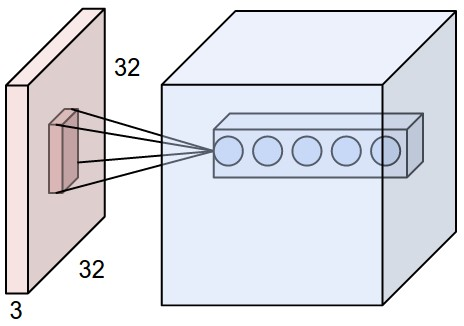
\includegraphics[page=1,width=0.40\textwidth]{depthcol.jpeg}
			\caption{\label{fig:conv_net}{The input volume in red is transformed into a set of 5 activation layers using 5 convolutional filters.\cite{stanford2016convnets}}}
		\end{figure}
		
		\noindent Even though powerful in many image processing applications, convolutional neural nets aren't the universal answer to all problems. The programmer possesses little control over what happens in the hidden features within them.
		
		\subsubsection{Summary and design choice}
		Having researched the various classification algorithms described above, we now faced the choice of either hand-designing features of the neuronal tissue scan or rather feeding the original image along with the labels into a CNN. Let's quickly review the available options. \\
		
		\noindent \textbf{Logistic regression} constitutes a simple and quick classification algorithm. Due to its simplicity, though, it is only applicable to linear models.
		
		\noindent \textbf{Random forests} along with the hand-designed features deal with the model non-linearities. They can potentially overfit the dataset, hence their performance was contrasted against that of neural networks on the dataset provided.
		
		\noindent \textbf{Neural networks} are often used in pattern recognition applications, and hence were thought to be a promising approach in our case. Their performance was however inferior to the random forests (recall: 12.5\% against 6\%).
		
		\noindent Finally, the \textbf{convolutional neural nets} seem to be a rising star in the pattern recognition application. Their insides are however hidden, and therefore hard to control. \\
		
		\noindent We felt like hand-designed features in conjunction with one of the classification methods might yield more promising results, as we can tailor the features so as to comply to our particular application. That is why, backed up by the recommendation of researchers from institutions such as EPFL and several papers (most notably Mischenko, 2009 \cite{mishchenko2009automation}, Chklovskii et al., 2010 \cite{chklovskii2010semi} or Navlakha et al., 2013 \cite{navlakha2013high}), we decided to \textbf{hand-design the features first} and try to obtain initial classification results with random forests and traditional neural nets. Both  have been tested using such an approach, and given the superior performance of the former, future design implementations will involve mainly \textbf{random forests}.\\
		
		\noindent This does not rule out prospective research into other classification algorithms, though. Hybrid combinations of random forests, neural nets and hand-designing features and CNN's should and will be tested to reveal the most accurate method.
		
		\subsection{Classification}
		
		As mentioned before, our choice of feeding our hand-designed features into a random forest was deemed as giving us more control and flexibility over the segmentation. That was also the method used by the researchers in several papers mentioned before.
		
		\subsubsection{Pixel-by-pixel classification}
		The abundance of data during classification might be an important factor determining its accuracy. The pixel-by-pixel method aims to achieve exactly that - by examining the immediate surrounding of an abundance of pixels we greatly expand the testing set and hence can better learn how to discern synapses in the validation set. \\
		Each pixel is surrounded by a window 70x70px, whose various geometrical and morphological features are extracted. Among those we calculate the color profiles, greyscale statistics, vesicle numbers or vesicles concentrations. Based on whether the pixel is part of a synapse or not, we then treat those features as either corresponding to a true or false label. \\
		
		\noindent The pixel-by-pixel classification is the most basic method researched and also the least effective one. The accuracy of the predictions did not exceed a few per cent when used in conjunction with random forests, and hence its improvements were forsaken for the more effective methods such as the regional classification described below.
		
		\subsubsection{Regional classification}
		Our most successful attempt at segmentation was a regional classification pipeline that can be summarized in a few simplified steps:
		
		\noindent \textbf{Training}
		\begin{enumerate}
			\item Preprocess the image in order to generate a collection of components that are candidates for synapses. This generates a lot of false positives (candidates that are not really synapses) and some true positives (candidates that are indeed synapses).
			\item Identify which of the generated candidates do indeed correspond to synapses using the validation dataset.
			\item Extract geometrical (morphological) features of the generated candidates such as area, perimeter, etc. In theory, the candidate synapses that possess a certain combination of features should indeed correspond to actual synapses.
			\item Run the classifier, in our case a bagged tree ensemble, on such features hoping to appropriately identify synapse existence based on candidate morphology.
		\end{enumerate}
		
		\noindent \textbf{Prediction}
		\begin{enumerate}
			\item Run the preprocessor again on the test set. Generate the candidates for synapses.
			\item Use the trained ensemble to decide which of the generated candidates correspond to synapses.
			\item Save only such candidates in the output image.
		\end{enumerate}
		
		\noindent One major assumption regarding this method is that our preprocessing algorithm is able to extract morphological features meaningful enough to differentiate the true synapse candidates. The image preprocessing pipeline needed for such classification is described below.
		
		\begin{figure}[!h]
			\centering
			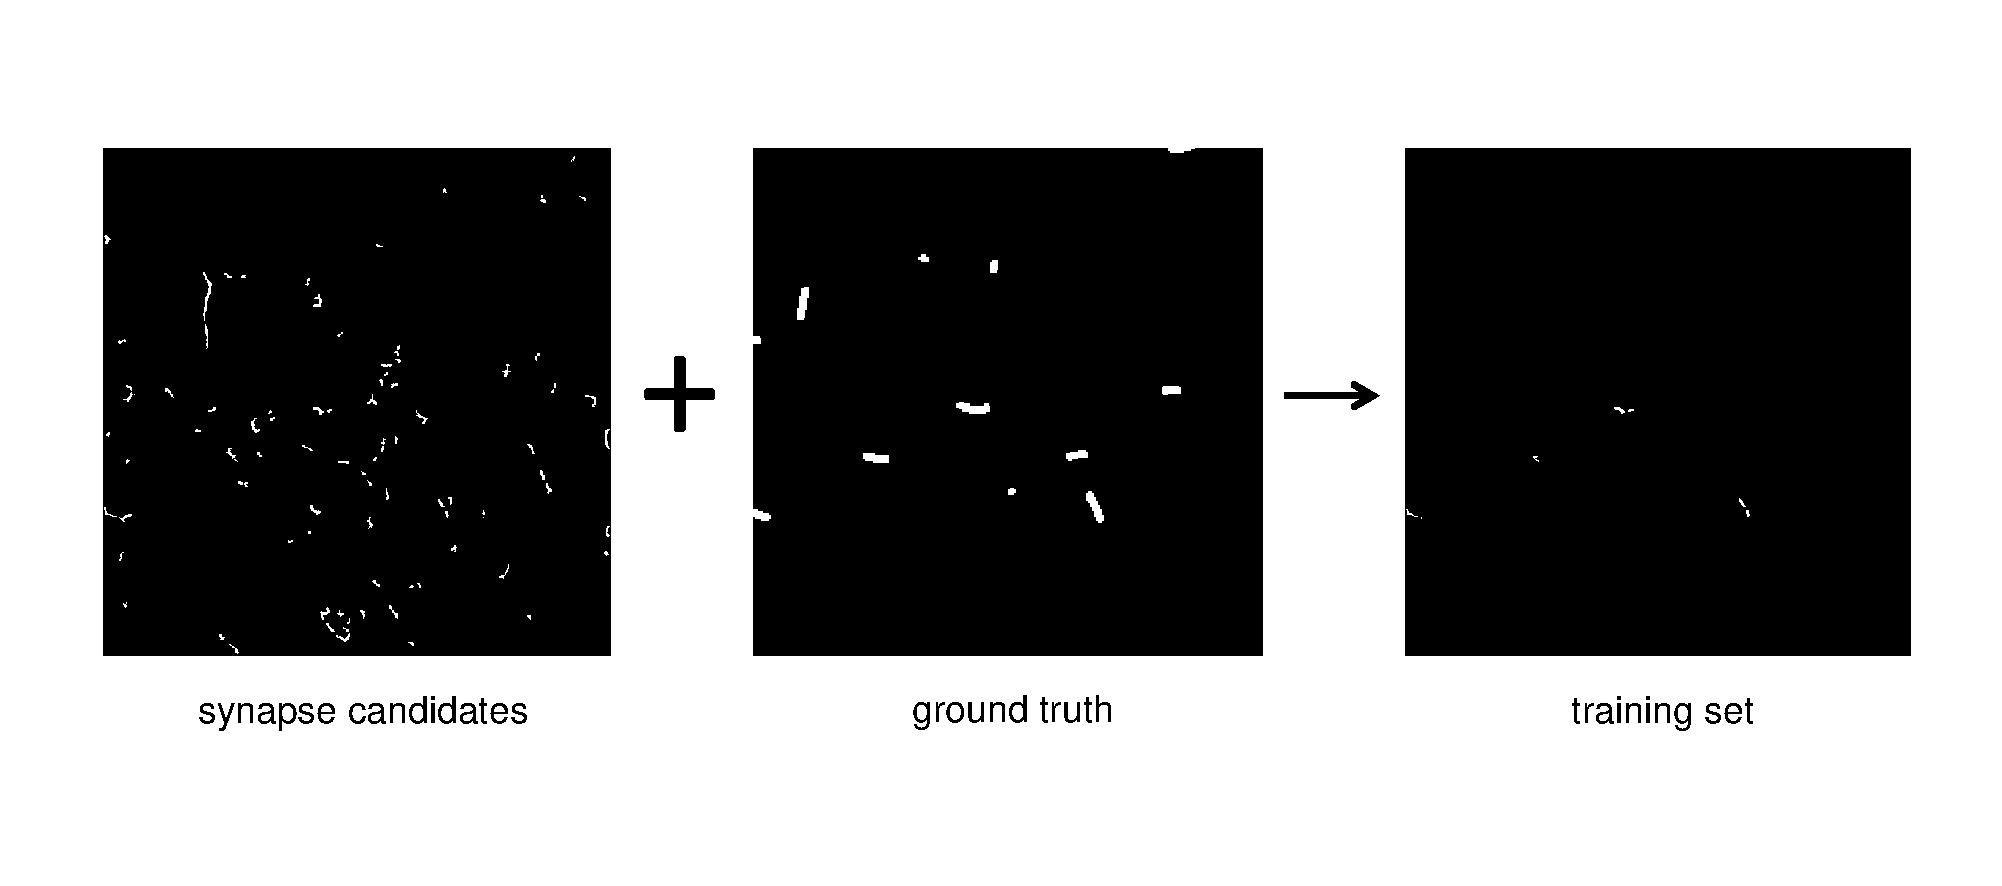
\includegraphics[page=1,width=0.70\textwidth]{segmentation_pipeline.pdf}
			\caption{\label{fig:segmentation_pipeline}{The synapse segmentation pipeline}}
		\end{figure}
		
		\subsubsection{Image preprocessing}
		
		The choice of our method i.e. generating the candidates for synapses and then training the set of their correspondence to the true classification, relies heavily on the former - appropriate generation method. To do this, we developed an intricate pipeline transforming the original image into one resembling the leftmost one in fig. \ref{fig:segmentation_pipeline}. This was based mostly on papers by Navlakha et al., 2013 \cite{navlakha2013high}, Bowyer at al., 2014 \cite{bowyer2014analysis} and Sklansky, 1978 \cite{sklansky1978image}.\\ 
		
		\begin{figure}[!ht]	
			\centering
			\begin{subfigure}[t]{.3\textwidth}
				\centering
				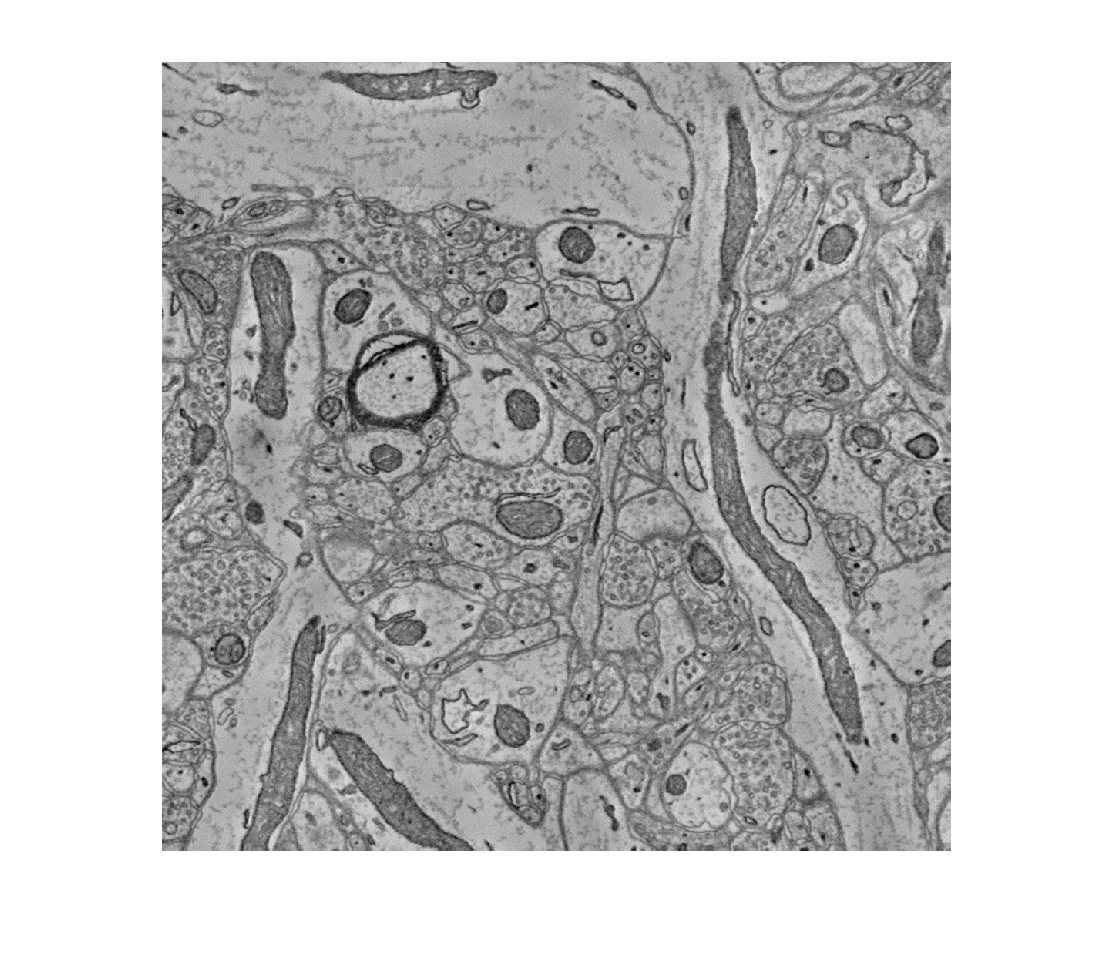
\includegraphics[width=\textwidth]{1_original}
				\caption{Original image}		
			\end{subfigure}
			\quad
			\begin{subfigure}[t]{.3\textwidth}
				\centering
				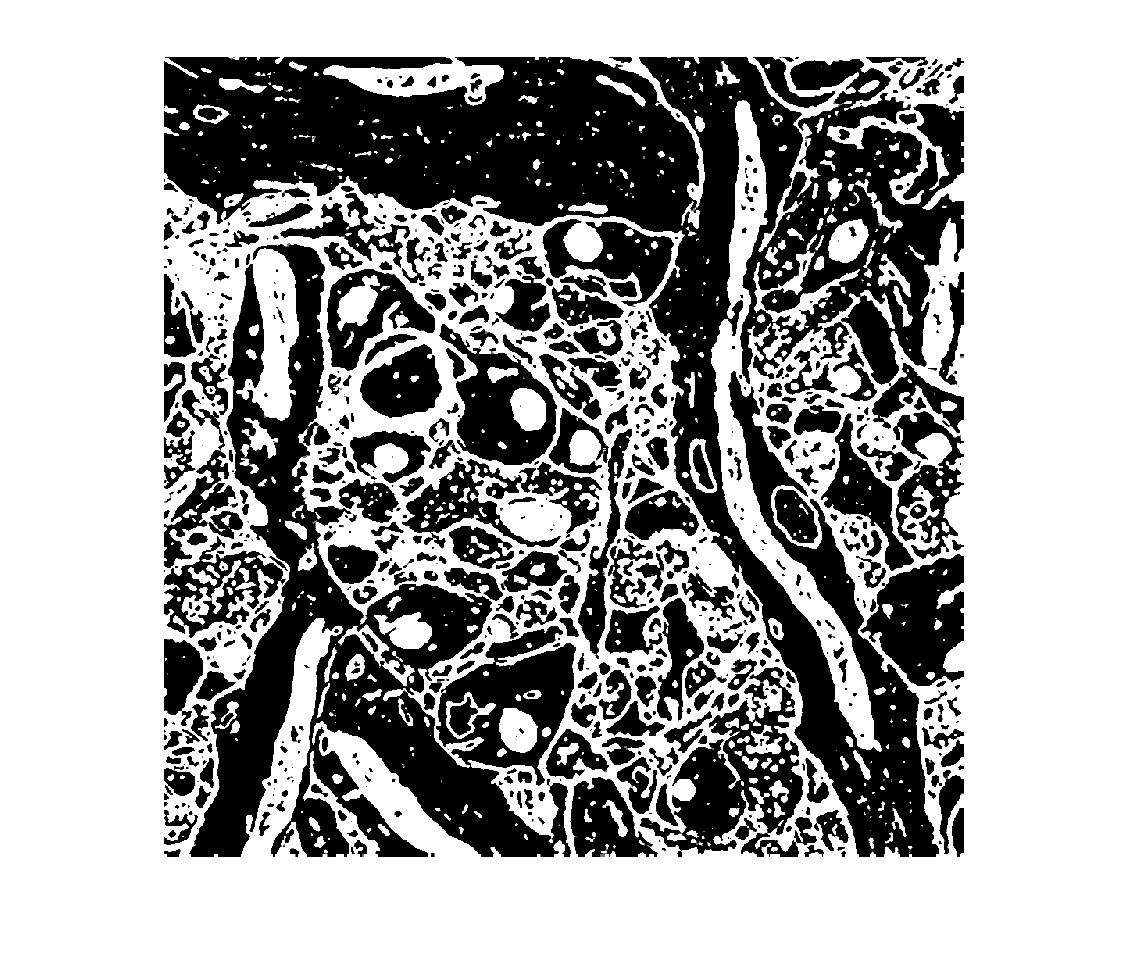
\includegraphics[width=\textwidth]{3_threshold}
				\caption{Binary equalised}
			\end{subfigure}
			\quad
			\begin{subfigure}[t]{.3\textwidth}
				\centering
				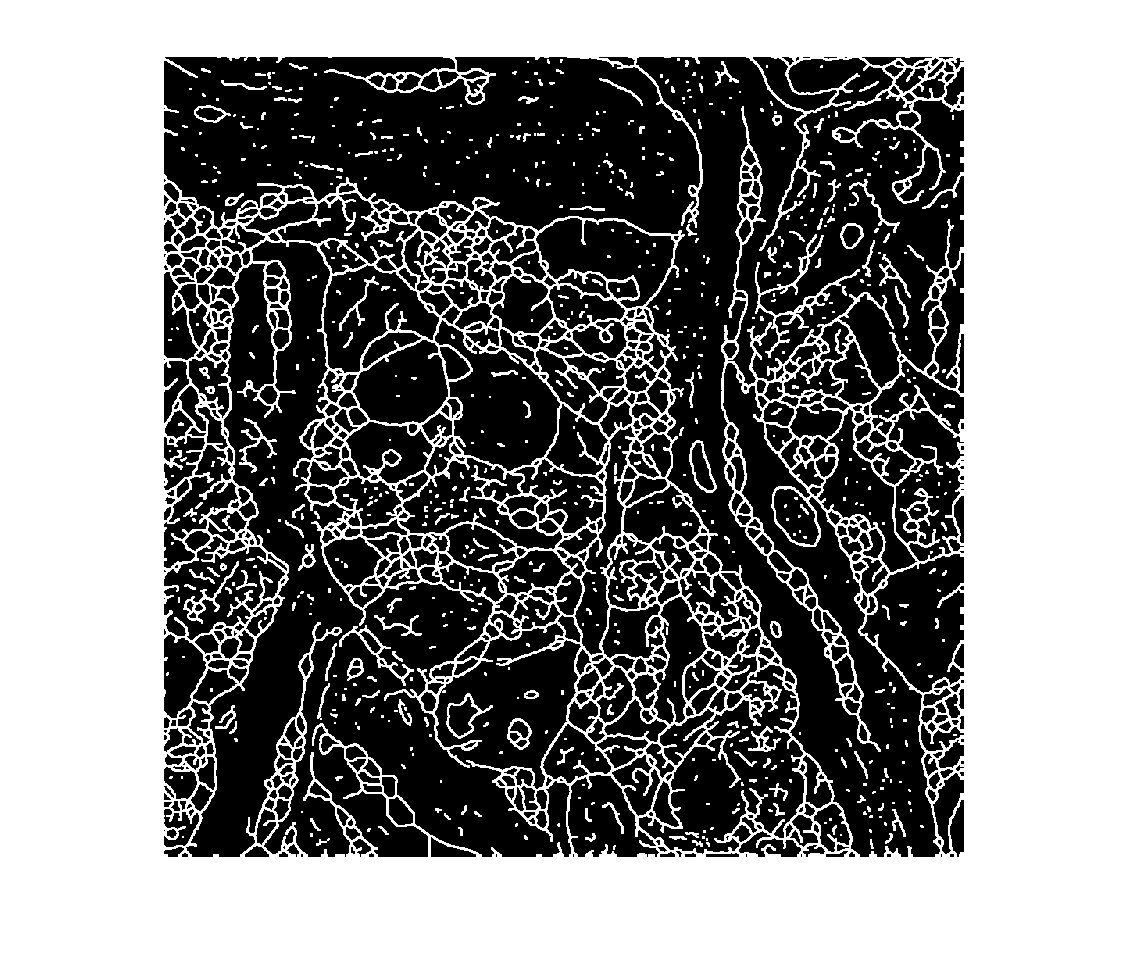
\includegraphics[width=\textwidth]{5_dilate}
				\caption{Dilated skeleton}
			\end{subfigure}
			\\
			\begin{subfigure}[t]{.3\textwidth}
				\centering
				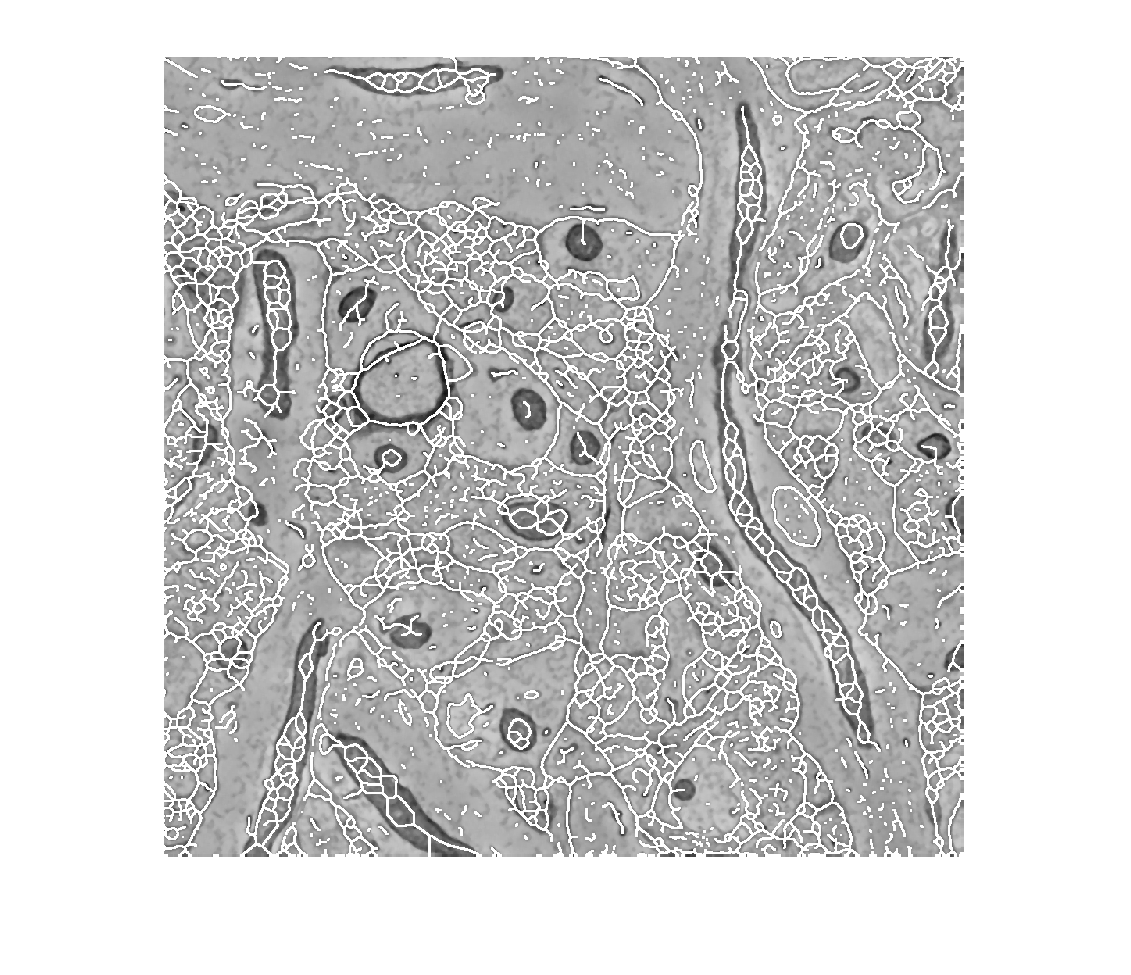
\includegraphics[width=\textwidth]{6_membranes_removed}
				\caption{Removed the membrane skeleton}
			\end{subfigure}
			\quad
			\begin{subfigure}[t]{.3\textwidth}
				\centering
				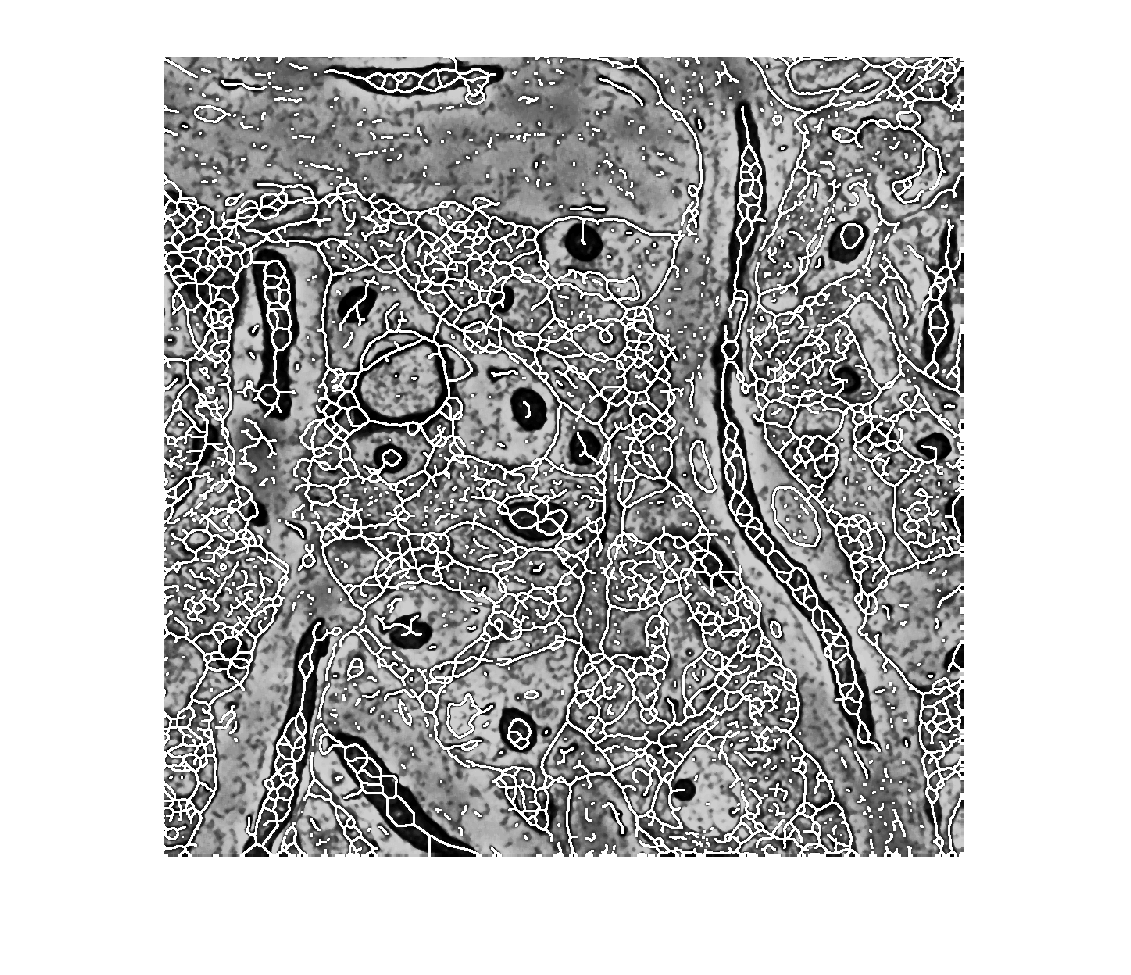
\includegraphics[width=\textwidth]{7_histeq}
				\caption{Histogram equalised}		
			\end{subfigure}
			\quad
			\begin{subfigure}[t]{.3\textwidth}
				\centering
				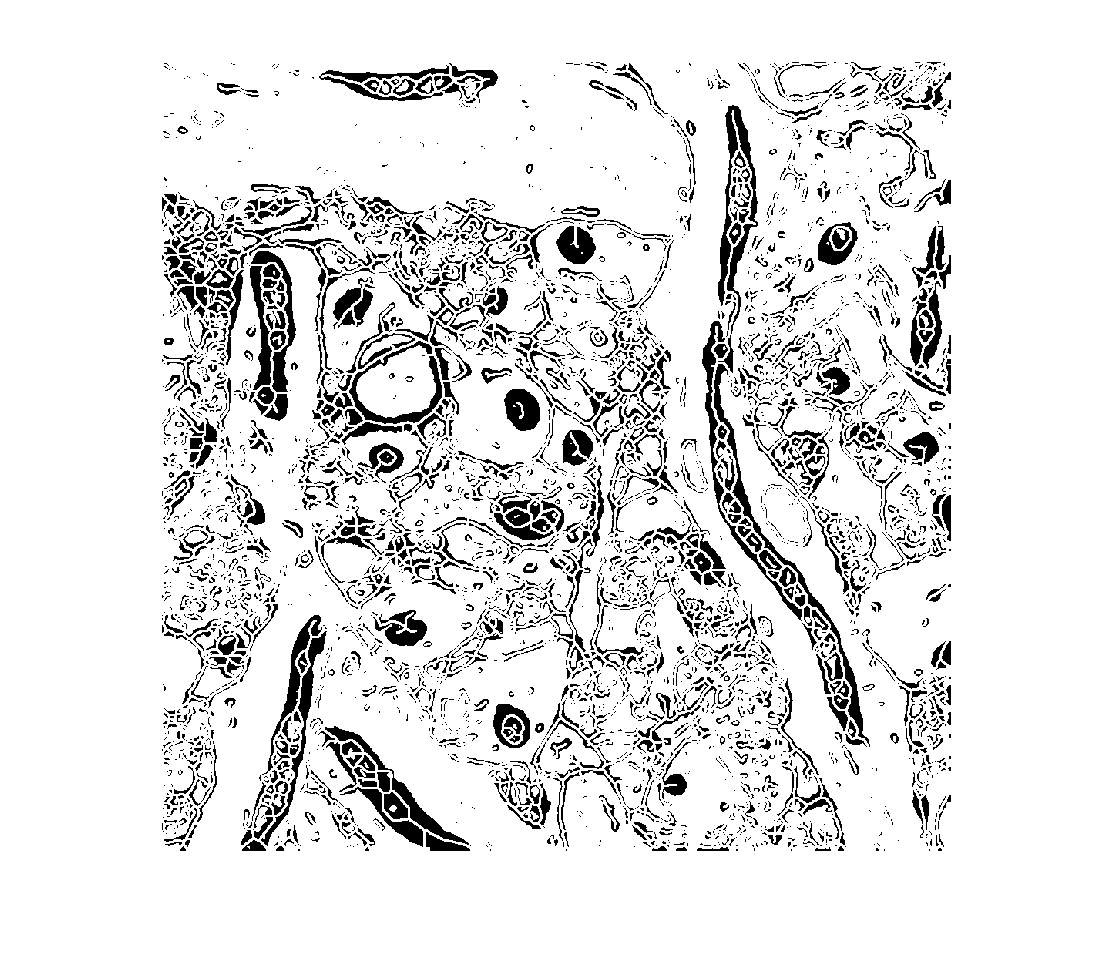
\includegraphics[width=\textwidth]{8_threshold}
				\caption{Thresholded}
			\end{subfigure}
			\\
			\begin{subfigure}[t]{.3\textwidth}
				\centering
				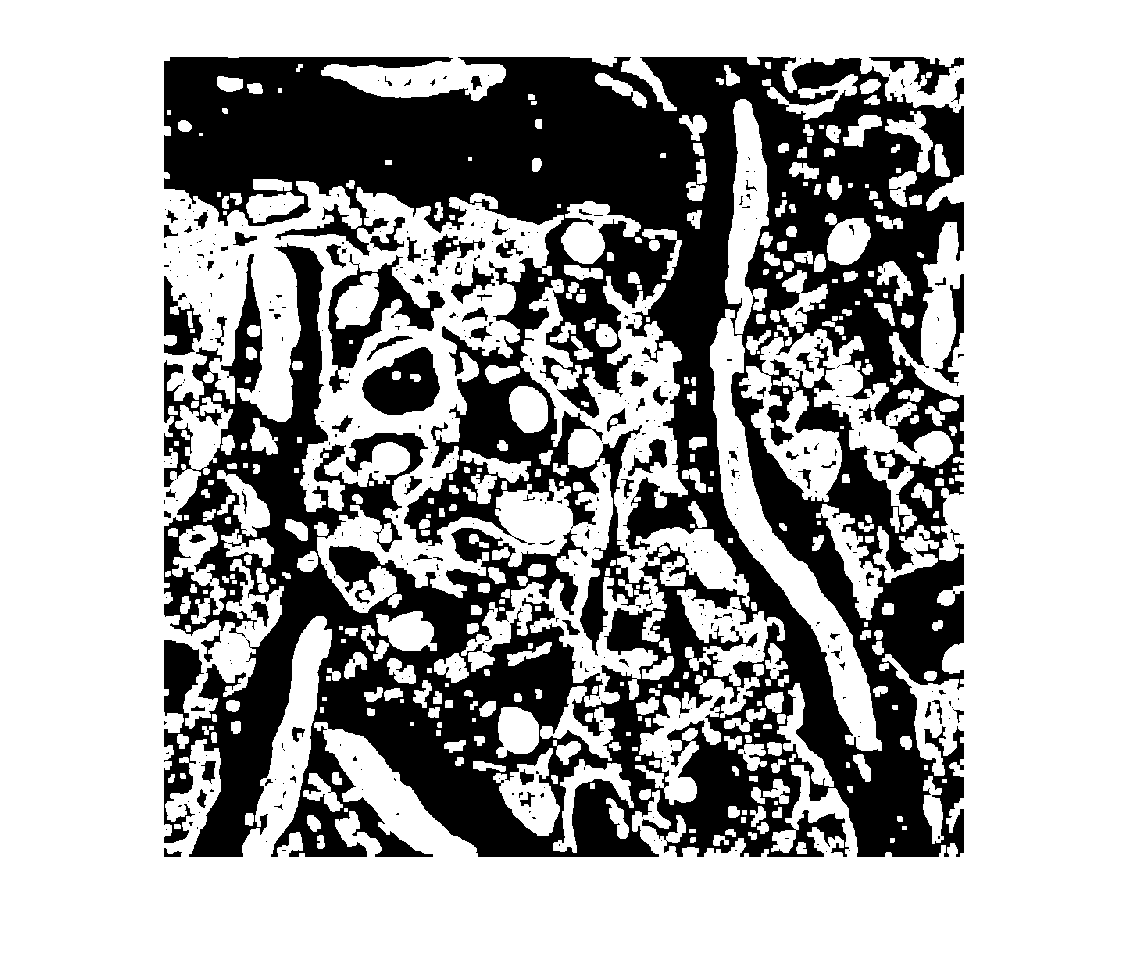
\includegraphics[width=\textwidth]{11_dilate}
				\caption{Dilated}
			\end{subfigure}
			\quad
			\begin{subfigure}[t]{.3\textwidth}
				\centering
				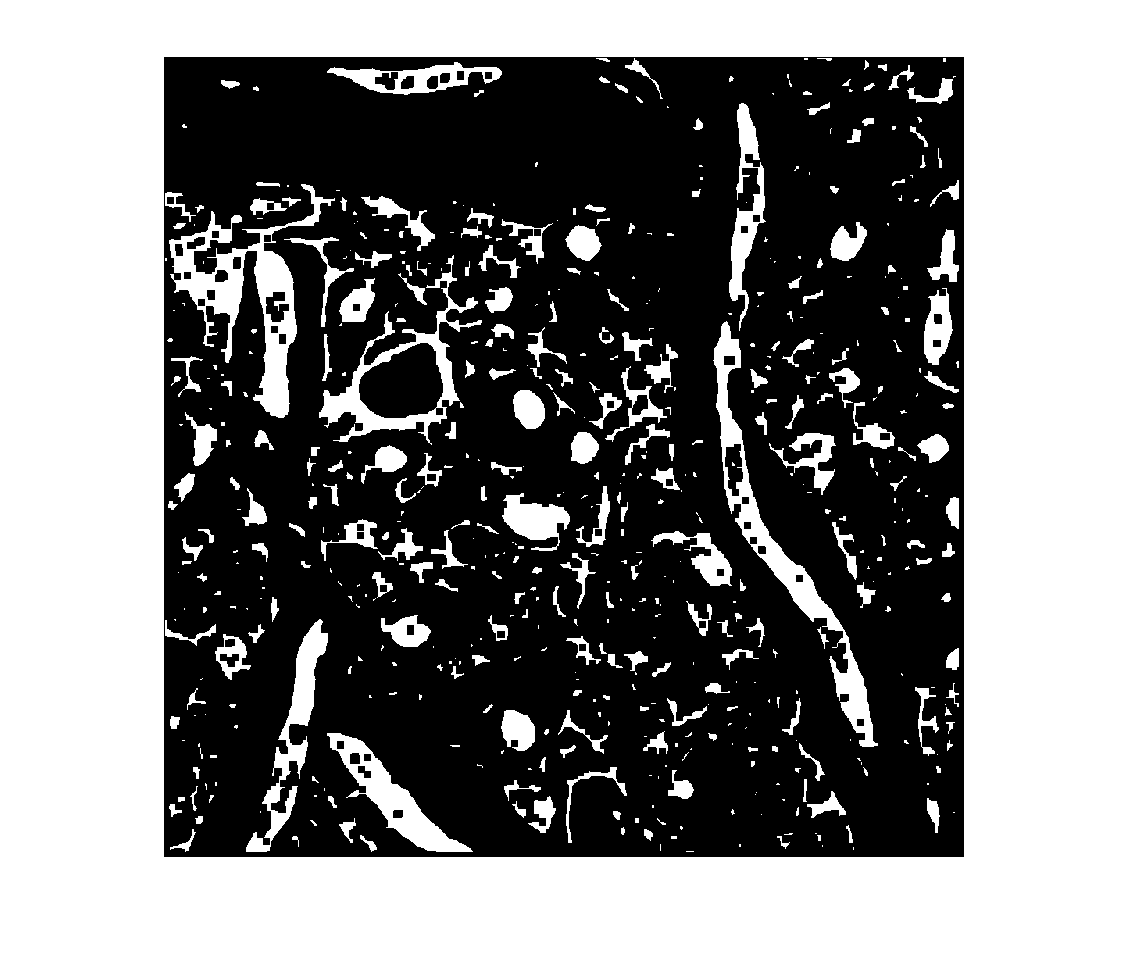
\includegraphics[width=\textwidth]{12_erode}
				\caption{Eroded}
			\end{subfigure}
			\quad
			\begin{subfigure}[t]{.3\textwidth}
				\centering
				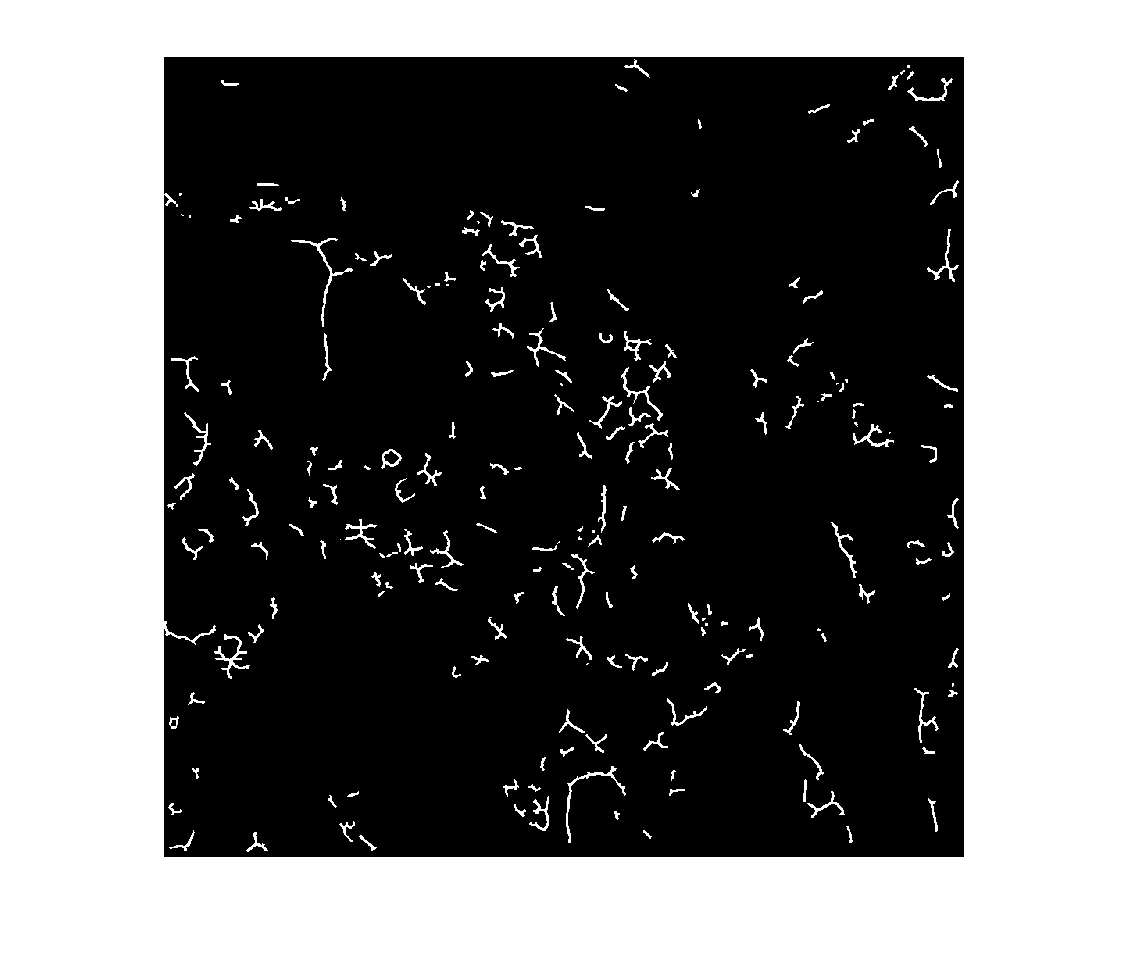
\includegraphics[width=\textwidth]{15_filtered}
				\caption{Filtered - \textbf{Final}}
			\end{subfigure}
			
			\caption{Image preprocessing pipeline}
			\label{fig:imagepreprocessing}
		\end{figure}
		
		\noindent The steps followed in order to obtain the image are as follows:
		\begin{enumerate}
			\item Median filter using a 5x5 pixel neighbourhood
			\item Binary equalize image using sample-independent threshold (fig. \ref{fig:imagepreprocessing} (b))
			\item In order to extract appropriate cell skeletons:
			\subitem Extract the skeleton of the binary equalised image (using MATLAB \textit{bwmorph})
			\subitem Dilate the skeleton (fig. \ref{fig:imagepreprocessing} (c))
			\item Remove the 'membrane' outline from the binary equalised image (fig. \ref{fig:imagepreprocessing} (d))
			\item Run histogram equalisation (fig. \ref{fig:imagepreprocessing} (e)) and thresholding to emphasise the synapse candidates (fig. \ref{fig:imagepreprocessing} (f))
			\item Apply the median filter again using 3x3 pixel neighbourhood
			\item Turn the image into black and white
			\item Dilate the leftover areas (fig. \ref{fig:imagepreprocessing} (g))
			\item Remove areas larger than and smaller than a chosen threshold
			\item Erode the leftover areas and run median the filter again (fig. \ref{fig:imagepreprocessing} (h))
			\item Set the output to only include areas which were the original membranes (fig. \ref{fig:imagepreprocessing} (i))
		\end{enumerate}
		
		\noindent This pipeline allowed us to produce the candidate synapses, whose geometrical properties were later used for training the classifier. The properties extracted were: area, perimeter, major axis length (for a corresponding ellipse), minor axis length, orientation, eccentricity (ratio of distance between the foci of the ellipse and its major axis length), convex area (number of pixels in the convex hull of the segment), diameter and extent (ratio of pixels in the segment to pixels in the smallest bounding box of the segment) \cite{navlakha2013high}.
		
		\subsection{Running time efficiency}
		As was mentioned in other places in the report, the bottleneck of the whole process pipeline, starting from brain preparation to storage, is the segmentation. During our investigation, it was established that even though training of the classifier was the most time consuming process (approximately an hour for a 100 layer tiff stack, corresponding to around $1300 \mu m^3$), the later classification wasn't as time-consuming. Even though the method was obviously imperfect, giving rather low F1 scores, the order of magnitude of the prediction time should not scale wildly with increasing accuracy. With that in mind, we can interpolate the test segmentation time to estimate the processing of the whole human brain like:
		\begin{equation} \label{segmtime}
		\textrm{segmentation time} = \frac{1400 \times (10^{-2})^3}{1278.7\times  \times (10^{-6})^3} \times 30 \textrm{minutes} = \textrm{62 million years}
		\end{equation}
		
		\noindent Clearly, this is still unreasonable. It has to be noted, however, that the physical processing power of GPUs/CPUs and algorithmic efficiency of the classifiers are increasing by orders of magnitude every year. This drastically improves the segmentation time estimate for the future. As an example, we can contrast the findings of two papers from different years analysing the automatic synapse segmentation:
		
		\begin{itemize}
			\item The Mishchenko paper from \textbf{2009} \cite{mishchenko2009automation} quotes values extrapolating to \boldmath$3.2 \times 10^{10}$ years of segmentation for one human brain
			\item The Chklovskii et al. paper from \textbf{2010} \cite{chklovskii2010semi} already reduces this figure to $4.3 \times 10^9$ years for an identical task.
		\end{itemize}
		
		\noindent Assuming a similar segmentation pace improvement year by year, the time required should drop to about 2 years of computation for a single human brain in 2023. Given the scale of our undertaking, this doesn't seem like an unreasonable figure - most probably just distant enough to get our business up and running anyways!
		
		\subsection{Hardware requirements}
		\label{Hardware}
		The recent years have seen an abrupt increase in the usage of GPUs (Graphical Processing Units) for computation. Thanks to the architecture of the GPUs, whose hundreds of cores support highly parallel computation, tasks such as image processing are greatly accelerated. This is the case also for machine learning applications - as researched by Raina et al. \cite{raina2009large} the performance of some learning models can be up to 70 times faster on GPUs compared to normal dual-core CPUs.\\
		
		\noindent The rise in popularity of GPU parallel computation was of course followed by increasing manufacturer support for such applications, with the most notable example being NVIDIA. Their CUDA computing platform, compatible with an array of popular programming languages, provides an easy way of harnessing the parallel computation potential of the GPUs \cite{nvidia2016cuda}. What is important from our perspective, CUDA support is also available in MATLAB, whose Parallel Computing Toolbox \cite{matlab2016cuda} provides a high level, easy access to the powerful NVIDIA framework.\\
		
		\noindent It is quite clear why the GPU is our hardware of choice when it comes to the computation itself. What is left is to calculate just how many and which of those GPUs we are going to need for our application. The most efficient NVIDIA GPU developed is Tesla K80, offering up to 2.91 Teraflops ($10^{12}$ floating operations per second) at around \pounds 7000 for a single unit. Running the classification using a bagged tree ensemble on 11 Intel Xeon E5-2620 CPU takes around one hour. A rough estimate of the number of floating point operations that can be performed on the machine has been obtained by calculating:
		
		\begin{equation}
		\textrm{flops/s} = \textrm{Number of Cores} \times \textrm{Average frequency} \times \textrm{Operations per cycle}
		\end{equation}
		
		\noindent Given our processor is 6-core with 2GHz clocking speed, 2 vector instructions/cycle and 4 simultaneous single-precision operands \cite{so2016flops} this gives around 176 Gigaflops. Coming back to equation \ref{segmtime}, since the time needed for a full segmentation of a human brain using such a processor is 62 million years, linearly scaling that through the computation power difference between our machine and one Tesla K80 ($\frac{2.91 \textrm{Teraflops}}{176 \textrm{Gigaflops}} = 16.53$) gives us about 3.75 million years. This of course drops to around 30 years if we decide to use \textbf{125 thousand} of K80's at a total cost of \textbf{\pounds 875 million}.  
		
		
		\newpage
			
		\clearpage
			
	\pagestyle{alex}
	
\section{Business Case}
\label{Business_Case}
\subsection{Executive Summary}

This report presents a method for saving a complete copy of the human brain for possible reanimation in the future. The research draws attention to the advances in technology, making it possible to fix, section and scan brain tissues to a great enough resolution to resolve synaptic strengths. 

We are currently seeking an investment of \pounds 20bn which will be required to start the business, purchasing all the necessary equipment to process the first human brain. In return we would be prepared to offer up to a 40\% stake in the company. 

Currently there is no other product like this on the market that allows the whole human brain to be saved. The closest alternative is cryogenics, the freezing of the entire body; however, this method has never been proven to work, and optimistic estimates of the first successful cryonic revival are 2045\footnote{http://zidbits.com/2011/02/can-a-human-be-frozen-and-brought-back-to-life [Accessed 08/03/2016]}. The market for cryogenics is rather small, with a handful of companies dominating the industry - ALCOR, Cryonic Institute and KrioRus being the largest three \cite{ftcryonics}. As of 2014, about 250 people were cryopreserved in the United States, with 1500 more having made arrangements for cryopreservation after their legal death\footnote{https://en.wikipedia.org/wiki/Cryonics [Accessed 08/03/2016]}.

We would look to charge prospective customers \pounds 5bn for the first 15 years, then reduce the price to \pounds 4bn for the next 5 years and finally charge \pounds 3bn after 20 years. We expect to make a profit by the 4th customer, 21 years after the formation of the firm. 

Due to the large costs of the method our target market will be any individual with a net worth of over \pounds 4bn (over 250). There has been significant interest from some of the world's wealthiest people, including Silvio Berlusconi (net worth \$7.7bn) planning to fund a research institute that will allow people to live until the age of 120 \cite{ftcryonics}. Whilst, Peter Thiel, PayPal founder (net worth \$3.3bn) and Simon Cowell (net worth \$550m) have already paid for a cryogenic operation on event of their death\footnote{www.forbes.com [Accessed 08/03/2016]}. We expect the market for saving oneself to grow over the coming years, particularly with the interest from high net worth individuals. 


\subsection{Benefits}

The benefits of this product are that there is a guarantee of saving the complete copy of the brain, providing the best chance of reanimation in the future. There is no other product quite like this in the market that provides the best chance of saving a brain as well as being scientifically supported by numerous medical papers.

People aged 60 and older make up 12.3\% of the global population, and by 2050, that number will rise to almost 22\%, due the increased size of developed nations. Consequently, the target market is constantly growing, as well as the number of people who can afford the treatment\footnote{http://www.unfpa.org/ageing [Accessed 08/03/2016]}.

By investing now, you have the chance to capture an entire sector, with a growing target market in a new, developing industry estimated to be worth \$21.09bn by 2019\footnote{http://www.marketsandmarkets.com/PressReleases/cryogenic.asp [Accessed 08/03/2016]}. In addition to providing a complete method for saving and processing a copy of the human brain, our firm will also provide a fixating brain service after death. As our method is scientifically proven to save the brain in the same state post-mortem, compared to cryogenics, we aim to capture a large section of the market.

\subsection{Risk}

Clearly some of the concerns involved are the costs of the method, however with the current rate of technical improvement, a 50\% percentage improvement in technology and 25\% percentage fall in costs is expected over 10 years. The process designed does involve ending a human life; however, as discussed previously the operation will be completed in a country that allows euthanasia by law. It is still a relatively new industry, although it is becoming more relevant as people now live longer.

\subsection{Timescale}

In order to complete the process within 10 years, a target set in order to balance the trade-off between processing time and cost, we will look to parallelise the process. The chemical preparation will take just over 140 hours to complete in order to ensure the first sample is ready for imaging and storage. This imaging process will run for approximately 10 years using 1,200 ATUMs, 12,000 SEM and 125,000 NVIDIA Tesla K80s machines.


\label{timescale}
\begin{figure}[H]
\centering
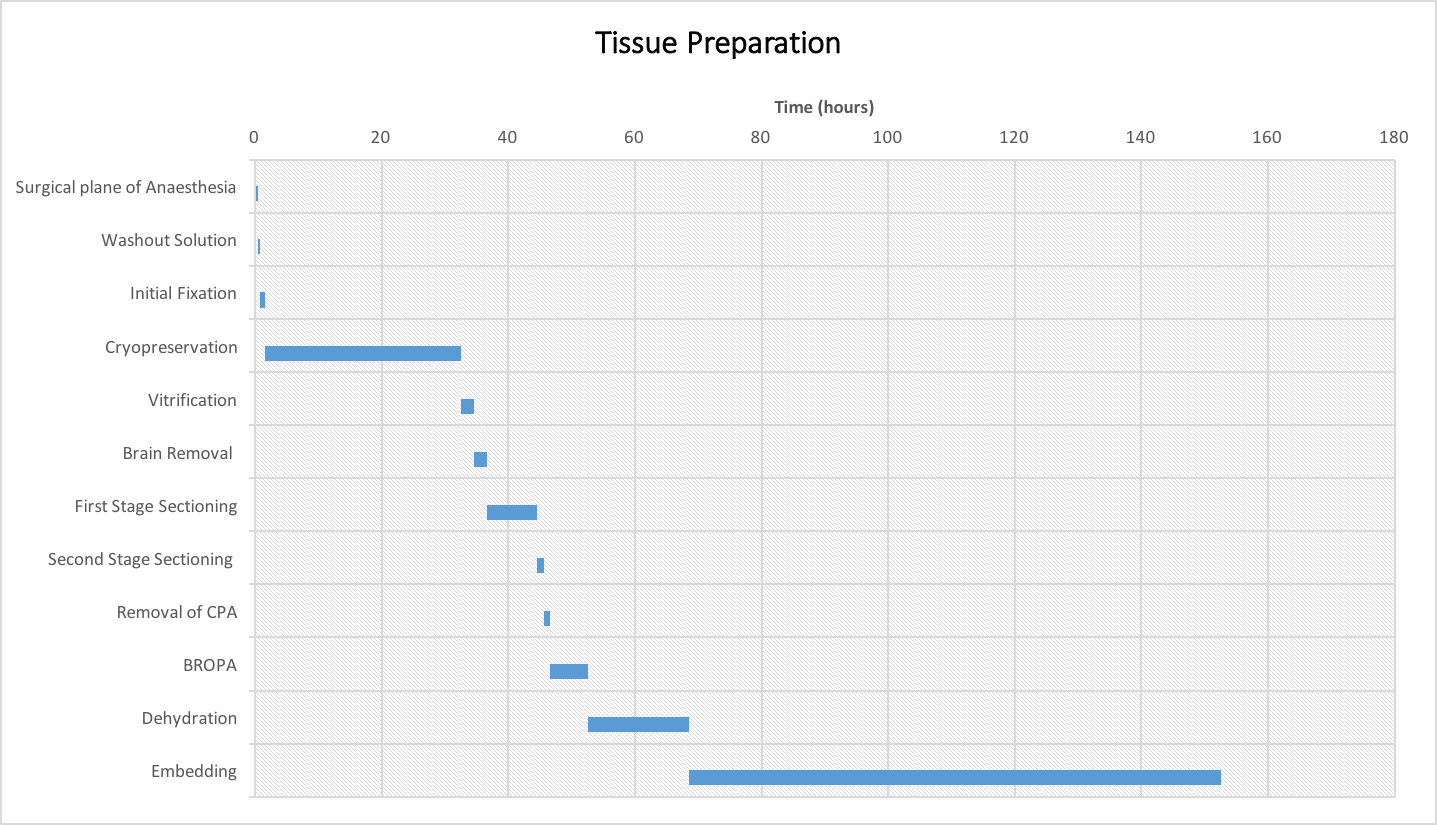
\includegraphics[width=0.80\textwidth]{tissueprep.png}
\caption{\label{fig:tissueprep} Tissue Preparation for One Sample}
\end{figure}	

\begin{figure}[H]
\centering
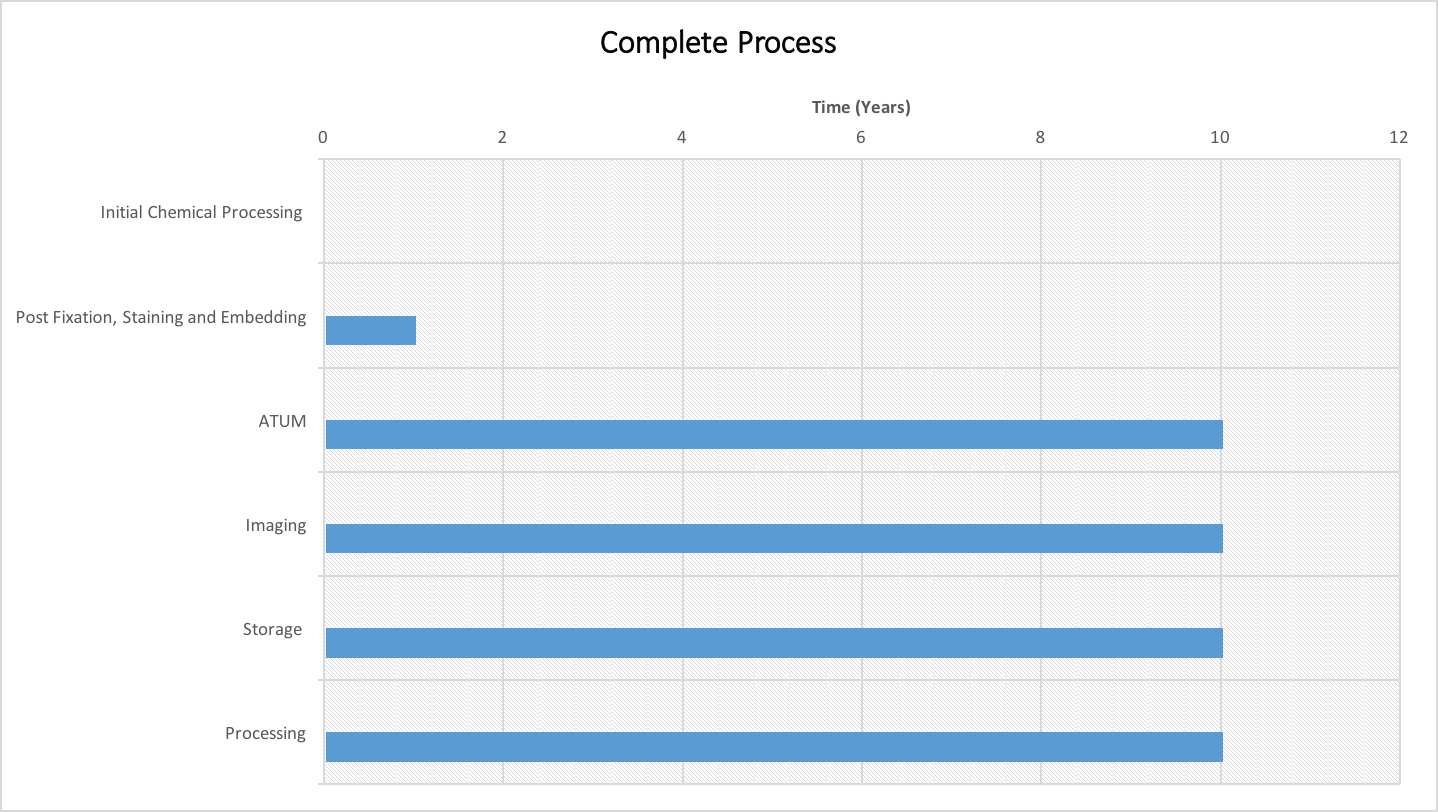
\includegraphics[width=0.80\textwidth]{Completeprocess.png}
\caption{\label{fig:tissueprep} Complete Process}
\end{figure}	


\subsection{Cost}

In the following tables a complete breakdown of costs for materials, machinery, utilities and labour can be seen for each of the significant stages of the process. 

\subsubsection{Materials}

Clearly the largest materials cost is the OCZ Vertex 4 hard drives, necessary for storing the large quantities of data. Of the remaining costs, the most expensive chemical is the osmium tetroxide; however this is necessary to ensure strong fixation and staining. The total cost of the materials for one person is therefore \pounds 151.1m.


\begin{table}[H]
\centering
\scalebox{0.6}{
\begin{tabular}{|l|l|l|l|l|}
\hline
\textbf{Stage} & \textbf{Material} & \textbf{Amount Required} & \textbf{Cost per Unit} & \textbf{Cost} \\ \hline

Surgical plane of Anaesthesia	&	Ketamine	&	\multicolumn{1}{r|}{	6.688mg	}	&	\multicolumn{1}{r|}{	\pounds	4.91/10ml	}	&	\multicolumn{1}{r|}{	\pounds	4.91	}	\\	\hline
	&	Xylazine	&	\multicolumn{1}{r|}{	836mg 	}	&	\multicolumn{1}{r|}{	\$33.92/50ml	}	&	\multicolumn{1}{r|}{	\pounds	370.95	}	\\	\hline
	&	Oxygen	&	\multicolumn{1}{r|}{	1L	}	&	\multicolumn{1}{r|}{	\pounds	83.56/L	}	&	\multicolumn{1}{r|}{	\pounds	83.56	}	\\	\hline
	&	Isoflurane	&	\multicolumn{1}{r|}{	0.05L	}	&	\multicolumn{1}{r|}{	\$34/250ml	}	&	\multicolumn{1}{r|}{	\pounds	15.70	}	\\	\hline
Washout Solution	&	Washout Solution	&	\multicolumn{1}{r|}{	15L	}	&	\multicolumn{1}{r|}{	\pounds	16.58/500ml	}	&	\multicolumn{1}{r|}{	\pounds	497.40	}	\\	\hline
Initial Fixation	&	Fixative Solution	&	\multicolumn{1}{r|}{	33.75L	}	&	\multicolumn{1}{r|}{	\pounds	278/L	}	&	\multicolumn{1}{r|}{	\pounds	9,452.00	}	\\	\hline
Cryopreservation	&	Fixative Solution	&	\multicolumn{1}{r|}{	11.2L	}	&	\multicolumn{1}{r|}{	\pounds	278.00/L	}	&	\multicolumn{1}{r|}{	\pounds	3,113.60	}	\\	\hline
	&	Ethylene Glycol	&	\multicolumn{1}{r|}{	20.8L	}	&	\multicolumn{1}{r|}{	\pounds	79.60/25L	}	&	\multicolumn{1}{r|}{	\pounds	91.70	}	\\	\hline
Vitrification	&	None	&	\multicolumn{1}{r|}{		}	&	\multicolumn{1}{r|}{	}	&	\multicolumn{1}{r|}{	\pounds 0.00	}	\\	\hline
Brain Removal 	&	None	&	\multicolumn{1}{r|}{		}	&	\multicolumn{1}{r|}{	}	&	\multicolumn{1}{r|}{	\pounds 0.00	}	\\	\hline
First Stage Sectioning	&	Agarose	&	\multicolumn{1}{r|}{	11kg	}	&	\multicolumn{1}{r|}{	\pounds 250.00/500g	}	&	\multicolumn{1}{r|}{	\pounds 5500	}	\\	\hline
Second Stage Sectioning 	&	None	&	\multicolumn{1}{r|}{		}	&	\multicolumn{1}{r|}{		}	&	\multicolumn{1}{r|}{	\pounds 0.00	}	\\	\hline
Removal of CPA	&	0.1 M cacodylate	&	\multicolumn{1}{r|}{	19l	}	&	\multicolumn{1}{r|}{	\pounds 88.3/100ml	}	&	\multicolumn{1}{r|}{	\pounds	16,777.00	}	\\	\hline
BROPA	&	Osmium tetroxide	&	\multicolumn{1}{r|}{	11.4kg	}	&	\multicolumn{1}{r|}{	\pounds 194.5/10ml	}	&	\multicolumn{1}{r|}{		\pounds 221,730.00	}	\\	\hline
	&	Potassium ferrocyanid	&	\multicolumn{1}{r|}{	4.9kg	}	&	\multicolumn{1}{r|}{	\pounds 7.17/100g	}	&	\multicolumn{1}{r|}{	\pounds	351.33	}	\\	\hline
	&	Sodium Cacodylate Buffer	&	\multicolumn{1}{r|}{	20.8kg	}	&	\multicolumn{1}{r|}{	\pounds	88.2/100ml	}	&	\multicolumn{1}{r|}{		\pounds 18,345.60	}	\\	\hline
	&	Formamide	&	\multicolumn{1}{r|}{	42g	}	&	\multicolumn{1}{r|}{	\pounds	35.63/100g	}	&	\multicolumn{1}{r|}{	\pounds	14.96	}	\\	\hline
	&	Pyrogallol	&	\multicolumn{1}{r|}{	15.3kg	}	&	\multicolumn{1}{r|}{	\pounds	120.50/500g	}	&	\multicolumn{1}{r|}{	\pounds	3,735.50	}	\\	\hline
Dehydration	&	Ethanol	&	\multicolumn{1}{r|}{	19L	}	&	\multicolumn{1}{r|}{	\pounds	265.06/2.5L	}	&	\multicolumn{1}{r|}{	\pounds	2,014.46	}	\\	\hline
Embedding	&	UNICRYL	&	\multicolumn{1}{r|}{	19L	}	&	\multicolumn{1}{r|}{	\pounds	237.15/250ml	}	&	\multicolumn{1}{r|}{	\pounds	18,023.40	}	\\	\hline
ATUM	&	Silicon wafers	&	\multicolumn{1}{r|}{	120,000	}	&	\multicolumn{1}{r|}{	\pounds 6.00	}	&	\multicolumn{1}{r|}{	\pounds 720,000	}	\\	\hline
	&	Kapton tape	&	\multicolumn{1}{r|}{	100,000	}	&	\multicolumn{1}{r|}{	\pounds 1.00	}	&	\multicolumn{1}{r|}{	\pounds	100,000.00}	\\	\hline
Imaging	&	None &	\multicolumn{1}{r|}{		}	&	\multicolumn{1}{r|}{			}	&	\multicolumn{1}{r|}{	\pounds 0.00	}	\\	\hline
Processing	&	None	&	\multicolumn{1}{r|}{		}	&	\multicolumn{1}{r|}{	}	&	\multicolumn{1}{r|}{	\pounds 0.00	}	\\	\hline
Storage 	&	OCZ Vertex 4                                               	&	\multicolumn{1}{r|}{	1,500,000	}	&	\multicolumn{1}{r|}{	\pounds	100.00	}	&	\multicolumn{1}{r|}{	\pounds	150,000,000.00	}	\\	\hline
 	&	  	&	& \textbf{Total}	&	\textbf{\pounds 151,120,122.07} \\	\hline
\end{tabular}
}
\captionsetup{justification=centering}
\caption{Cost of Materials}
\label{table:materialcosts}
\end{table}

\subsubsection{Machinery}

The machinery cost, which makes up 97.6\% of the total cost of the project, is so high due to the highly specialised machines required. The maintenance cost is calculated as 5\% of the value of the machine\footnote{www.open.edu [Accessed 17/04/2016]}. The initial cost and maintenance cost are calculated per unit, summed together to generate the total cost for each type of machinery. 





\begin{table}[H]
\centering
\scalebox{0.5}{
\begin{tabular}{ | l | l | l | l | l | l | l | }
\hline
	
	\textbf{Stage} & \textbf{Machinery} & \textbf{Quantity} & \textbf{Price/Unit} & \textbf{Maintenance Cost} & \textbf{Total Cost/Unit} & \textbf{Total Cost}  \\ \hline
	Surgical plane of Anaesthesia	&	None	&	\multicolumn{1}{r|}{		}	&	\multicolumn{1}{r|}{				}				&	\multicolumn{1}{r|}{			}	&	\multicolumn{1}{r|}{			}	&	\multicolumn{1}{r|}{		\pounds 0.00	}	\\	\hline
Washout Solution	&	Manual Perfusion Machine	&	\multicolumn{1}{r|}{	1	}	&	\multicolumn{1}{r|}{	\pounds	5,000.00		}				&	\multicolumn{1}{r|}{	\pounds	250.00	}	&	\multicolumn{1}{r|}{	\pounds	5,250.00	}	&	\multicolumn{1}{r|}{	\pounds	5,250.00	}	\\	\hline
Initial Fixation	&	Automated Perfusion Machine 	&	\multicolumn{1}{r|}{	1	}	&	\multicolumn{1}{r|}{	\pounds	10,000.00		}				&	\multicolumn{1}{r|}{	\pounds	500.00	}	&	\multicolumn{1}{r|}{	\pounds	10,500.00	}	&	\multicolumn{1}{r|}{	\pounds	10,500.00	}	\\	\hline
Cryopreservation	&	 Vapour Storage Unit	&	\multicolumn{1}{r|}{	1	}	&	\multicolumn{1}{r|}{	\pounds	10,000.00		}				&	\multicolumn{1}{r|}{	\pounds	500.00	}	&	\multicolumn{1}{r|}{	\pounds	10,500.00	}	&	\multicolumn{1}{r|}{	\pounds	10,500.00	}	\\	\hline
Vitrification	&	None	&	\multicolumn{1}{r|}{		}	&	\multicolumn{1}{r|}{				}				&	\multicolumn{1}{r|}{			}	&	\multicolumn{1}{r|}{			}	&	\multicolumn{1}{r|}{	\pounds 0.00		}	\\	\hline
Brain Removal 	&	Stryker M810	&	\multicolumn{1}{r|}{	1	}	&	\multicolumn{1}{r|}{	\pounds	3,000.00		}				&	\multicolumn{1}{r|}{	\pounds	150.00	}	&	\multicolumn{1}{r|}{	\pounds	3,150.00	}	&	\multicolumn{1}{r|}{	\pounds	3,150.00	}	\\	\hline
First Stage Sectioning	&	Compresstome	&	\multicolumn{1}{r|}{	1	}	&	\multicolumn{1}{r|}{	\pounds	46,000.00		}				&	\multicolumn{1}{r|}{	\pounds	2,300.00	}	&	\multicolumn{1}{r|}{	\pounds	48,300.00	}	&	\multicolumn{1}{r|}{	\pounds	48,300.00	}	\\	\hline
Second Stage Sectioning 	&	Custom Vibratome	&	\multicolumn{1}{r|}{	1	}	&	\multicolumn{1}{r|}{	\pounds	20,000.00		}				&	\multicolumn{1}{r|}{	\pounds	1,000.00	}	&	\multicolumn{1}{r|}{	\pounds	21,000.00	}	&	\multicolumn{1}{r|}{	\pounds	21,000.00	}	\\	\hline
Chemical Processing	&	Lynx II for Microscopy	&	\multicolumn{1}{r|}{	170	}	&	\multicolumn{1}{r|}{	\pounds	13,750.00		}				&	\multicolumn{1}{r|}{	\pounds	6875.00	}	&	\multicolumn{1}{r|}{	\pounds	20,625.00	}	&	\multicolumn{1}{r|}{	\pounds	3,506,250.00	}	\\	\hline
ATUM	&	ATUMtome	&	\multicolumn{1}{r|}{	1200	}	&	\multicolumn{1}{r|}{	\pounds	50,000.00		}				&	\multicolumn{1}{r|}{	\pounds	25,000.00	}	&	\multicolumn{1}{r|}{	\pounds	75,000.00	}	&	\multicolumn{1}{r|}{	\pounds	90,000,000.00	}	\\	\hline
Imaging	&	Robotic Arm Autoloader 	&	\multicolumn{1}{r|}{	12,000	}	&	\multicolumn{1}{r|}{	\pounds	10,000.00		}				&	\multicolumn{1}{r|}{	\pounds	5,000.00	}	&	\multicolumn{1}{r|}{	\pounds	15,000.00	}	&	\multicolumn{1}{r|}{	\pounds	180,000,000.00	}	\\	\hline
	&	ZEISS MultiSEM 506 and Axio Imager A2 Vario	&	\multicolumn{1}{r|}{	12,000	}	&	\multicolumn{1}{r|}{	\pounds	2,565,000		}				&	\multicolumn{1}{r|}{	\pounds	135,000.00	}	&	\multicolumn{1}{r|}{	\pounds	2,700,000.00	}	&	\multicolumn{1}{r|}{	\pounds	32,400,000,000.00	}	\\	\hline
Processing	&	NVIDIA Tesla K80	&	\multicolumn{1}{r|}{	125,000	}	&	\multicolumn{1}{r|}{	\pounds	7,000.00		}				&	\multicolumn{1}{r|}{	\pounds	3,500.00	}	&	\multicolumn{1}{r|}{	\pounds	10,500.00	}	&	\multicolumn{1}{r|}{	\pounds	1,312,500,000.00	}	\\	\hline
Storage 	&	None	&	\multicolumn{1}{r|}{		}	&	\multicolumn{1}{r|}{				}				&	\multicolumn{1}{r|}{			}	&	\multicolumn{1}{r|}{			}	&	\multicolumn{1}{r|}{\pounds 0.00			}	\\	\hline

 	&		&	\multicolumn{1}{r|}{		}	&	\multicolumn{1}{r|}{				}				&	\multicolumn{1}{r|}{			}	&	\multicolumn{1}{r|}{		\textbf{Total}	}	&	\multicolumn{1}{r|}{	\textbf{\pounds 33,986,104,950.00}		}	\\	\hline

\end{tabular}
}
\captionsetup{justification=centering}
\caption{Cost of Machinery}
\label{table:machinecost}
\end{table}

\subsubsection{Utilities}

For the utilities section, we only calculated power and rent for the chemical processing, ATUM, imaging, processing and storage due to the insignificant cost of the other stages. This was assumed to be \pounds 20,000 to rent a laboratory for one week\footnote{https://www.abtech.edu/content/BioNetwork/Laboratory-Use-amp-Equipment-Rental [Accessed 02/05/2016]}. The power consumption figures were taken from the manufactures specification and the cost of power calculated using 1kWh costing \pounds 0.066\footnote{https://www.gov.uk/government/uploads/system/uploads/attachment\_data/file/511316/QEP\_Mar\_2016\_V2.pdf" [Accessed 02/05/2016]}.


\begin{table}[H]
\centering
\scalebox{0.6}{
\begin{tabular}{|l|l|l|l|l|l|l|}
\hline
\textbf{Stage}	&		\begin{tabular}{@{}c@{}}\textbf{Power Consumption/} \\ \textbf{Machine}\end{tabular}		&			\begin{tabular}{@{}c@{}}\textbf{Power Cost/} \\ \textbf{Machine}\end{tabular}		&		\textbf{Area Required}							&			\textbf{Rent/Machine}	&			\textbf{Total/Machine}		&			\textbf{Total Cost} 		\\	\hline
Pre Chemical Processing	&			&	\multicolumn{1}{r|}{			}	&	\multicolumn{1}{r|}{					}				&	\multicolumn{1}{r|}{			}	&	\multicolumn{1}{r|}{			}	&	\multicolumn{1}{r|}{	\pounds	20,000.00	}	\\	\hline
Chemical Processing	&	\multicolumn{1}{r|}{	1.0kW	}	&	\multicolumn{1}{r|}{	\pounds	525.60	}	&	\multicolumn{1}{r|}{	3.000m	$	^2	$	}				&	\multicolumn{1}{r|}{	\pounds	77.13	}	&	\multicolumn{1}{r|}{	\pounds	602.73	}	&	\multicolumn{1}{r|}{	\pounds	102,464.10	}	\\	\hline
ATUM	&	\multicolumn{1}{r|}{	1.0kW	}	&	\multicolumn{1}{r|}{	\pounds	5,256.00	}	&	\multicolumn{1}{r|}{	1.000m	$	^2	$	}				&	\multicolumn{1}{r|}{	\pounds	257.10	}	&	\multicolumn{1}{r|}{	\pounds	5,513.10	}	&	\multicolumn{1}{r|}{	\pounds	6,615,720.00	}	\\	\hline
Imaging	&	\multicolumn{1}{r|}{	1.0kW	}	&	\multicolumn{1}{r|}{	\pounds	5,781.60	}	&	\multicolumn{1}{r|}{	1.000m	$	^2	$	}				&	\multicolumn{1}{r|}{	\pounds	257.10	}	&	\multicolumn{1}{r|}{	\pounds	6,038.70	}	&	\multicolumn{1}{r|}{	\pounds	72,464,400.00	}	\\	\hline
	&	\multicolumn{1}{r|}{	4.5kW	}	&	\multicolumn{1}{r|}{	\pounds	26,017.20	}	&	\multicolumn{1}{r|}{	20.000m	$	^2	$	}				&	\multicolumn{1}{r|}{	\pounds	5,142.00	}	&	\multicolumn{1}{r|}{	\pounds	31,159.20	}	&	\multicolumn{1}{r|}{	\pounds	373,910,400.00	}	\\	\hline
Processing	&	\multicolumn{1}{r|}{	0.3kW	}	&	\multicolumn{1}{r|}{	\pounds	1,734.48	}	&	\multicolumn{1}{r|}{	0.004m	$	^2	$	}				&	\multicolumn{1}{r|}{	\pounds	1.03	}	&	\multicolumn{1}{r|}{	\pounds	1,735.51	}	&	\multicolumn{1}{r|}{	\pounds	216,938,550.00	}	\\	\hline
Storage 	&	\multicolumn{1}{r|}{	2.5kW	}	&	\multicolumn{1}{r|}{	\pounds	14.45	}	&	\multicolumn{1}{r|}{	0.004m	$	^2	$	}				&	\multicolumn{1}{r|}{	\pounds	1.03	}	&	\multicolumn{1}{r|}{	\pounds	15.48	}	&	\multicolumn{1}{r|}{	\pounds	23,223,600.00	}	\\	\hline

 	&		&	\multicolumn{1}{r|}{		}	&	\multicolumn{1}{r|}{				}				&	\multicolumn{1}{r|}{			}	&	\multicolumn{1}{r|}{		\textbf{Total}	}	&	\multicolumn{1}{r|}{	\textbf{\pounds 693,275,134.10}		}	\\	\hline

\end{tabular}
}
\captionsetup{justification=centering}
\caption{Cost of Utilities}
\label{table:Utilitiescost}
\end{table}




\subsubsection{Labour}

For the labour section, we looked at the wage requirement of the staff to complete the pipeline. From the below table clearly the largest costs are associated with the processes that take the longest to complete, usually requiring the most highly trained and therefore most expensive staff in terms of wage. 

\begin{table}[H]
\centering
\scalebox{0.7}{
\begin{tabular}{|l|l|l|l|l|l|l|}
\hline
\textbf{Stage}	&		\textbf{Profession}		&			\textbf{Quantity Required	}	&			\textbf{Wage		}					&		\textbf{	Total Cost	}	\\	\hline
Surgical plane of Anaesthesia	&		Skilled surgeon 		&	\multicolumn{1}{r|}{		1	}	&	\multicolumn{1}{r|}{	\pounds	75.00	/hour		}				&	\multicolumn{1}{r|}{	\pounds	35.00	}	\\	\hline
	&		Lab Assistant 		&	\multicolumn{1}{r|}{		2	}	&	\multicolumn{1}{r|}{	\pounds	7.21/hour			}				&	\multicolumn{1}{r|}{	\pounds	7.21	}	\\	\hline
Washout Solution	&		Lab Assistant 		&	\multicolumn{1}{r|}{		2	}	&	\multicolumn{1}{r|}{	\pounds	7.21/hour			}				&	\multicolumn{1}{r|}{	\pounds	4.76	}	\\	\hline
Initial Fixation	&		Lab Assistant 		&	\multicolumn{1}{r|}{		2	}	&	\multicolumn{1}{r|}{	\pounds	7.21/hour			}				&	\multicolumn{1}{r|}{	\pounds	10.82	}	\\	\hline
Cryopreservation	&		Lab Assistant 		&	\multicolumn{1}{r|}{		1	}	&	\multicolumn{1}{r|}{	\pounds	7.21/hour			}				&	\multicolumn{1}{r|}{	\pounds	49.91	}	\\	\hline
Vitrification	&		Lab Assistant 		&	\multicolumn{1}{r|}{		1	}	&	\multicolumn{1}{r|}{	\pounds	7.21/hour			}				&	\multicolumn{1}{r|}{	\pounds	14.42	}	\\	\hline
Brain Removal 	&		Skilled surgeon 		&	\multicolumn{1}{r|}{		1	}	&	\multicolumn{1}{r|}{	\pounds	75.00/hour			}				&	\multicolumn{1}{r|}{	\pounds	150.00	}	\\	\hline
First Stage Sectioning	&		Lab Assistant 		&	\multicolumn{1}{r|}{		1	}	&	\multicolumn{1}{r|}{	\pounds	7.21/hour			}				&	\multicolumn{1}{r|}{	\pounds	57.68	}	\\	\hline
Second Stage Sectioning 	&		Lab Assistant 		&	\multicolumn{1}{r|}{		1	}	&	\multicolumn{1}{r|}{	\pounds	7.21/hour			}				&	\multicolumn{1}{r|}{	\pounds	7.21	}	\\	\hline
Chemical Processing	&		Lab Assistant 		&	\multicolumn{1}{r|}{		30	}	&	\multicolumn{1}{r|}{	\pounds	15,000/year			}				&	\multicolumn{1}{r|}{	\pounds	450,000.00	}	\\	\hline
ATUM	&		Lab Assistant 		&	\multicolumn{1}{r|}{		6	}	&	\multicolumn{1}{r|}{	\pounds	15,000/year			}				&	\multicolumn{1}{r|}{	\pounds	900,000.00	}	\\	\hline
Imaging	&		Engineer		&	\multicolumn{1}{r|}{		10	}	&	\multicolumn{1}{r|}{	\pounds	50,000/year			}				&	\multicolumn{1}{r|}{	\pounds	5,000,000.00	}	\\	\hline
Processing	&		Developer		&	\multicolumn{1}{r|}{		5	}	&	\multicolumn{1}{r|}{	\pounds	50,000/year			}				&	\multicolumn{1}{r|}{	\pounds	2500,000.00	}	\\	\hline
Storage 	&		Lab Technician		&	\multicolumn{1}{r|}{		2	}	&	\multicolumn{1}{r|}{	\pounds	15,000/year			}				&	\multicolumn{1}{r|}{	\pounds	300,000.00	}	\\	\hline


 	&		&		&	\multicolumn{1}{r|}{		\textbf{Total}	}	&	\multicolumn{1}{r|}{	\textbf{\pounds 9,150,337.00}		}	\\	\hline

\end{tabular}
}
\captionsetup{justification=centering}
\caption{Cost of Labour}
\label{table:labourcost}
\end{table}



\subsubsection{Total}

The total overall cost is derived by summing the previously calculated  cost components. The final cost for completely saving one brain is \pounds 35.98bn, which takes just under 10 years. The number of machines used to achieve this could be increased to reduce production time; however, due to the already high cost of this process as well as the technology needed to reanimate the brain not being fully developed yet, this would not be practical. 
 

\begin{table}[H]
\centering
\scalebox{0.7}{
\begin{tabular}{|l|r|r|r|r|r|}
\hline
                              & \multicolumn{1}{l|}{Material} & \multicolumn{1}{l|}{Machinery} & \multicolumn{1}{l|}{Utilities} & \multicolumn{1}{l|}{Labour}  & \multicolumn{1}{l|}{Total Cost} \\ \hline
Surgical plane of Anaesthesia & \pounds 475.12                       & \pounds 0                             & \multirow{8}{*}{\pounds 20,000}       & \pounds 42.21                       & \pounds 3017.33                        \\ \cline{1-3} \cline{5-6} 
Washout Solution              & \pounds 497.40                       & \pounds 5,250.00                      &                                & \pounds 4.76                        & \pounds 8252.16                        \\ \cline{1-3} \cline{5-6} 
Initial Fixation              & \pounds 9,452.00                     & \pounds 10,500.00                     &                                & \pounds 10.82                       & \pounds 22462.82                       \\ \cline{1-3} \cline{5-6} 
Cryopreservation              & \pounds 3,205.30                     & \pounds 10,500.00                     &                                & \pounds 49.91                       & \pounds 16255.21                       \\ \cline{1-3} \cline{5-6} 
Vitrification                 & \pounds 0.00                         & \pounds 0.00                          &                                & \pounds 14.42                       & \pounds 2514.42                        \\ \cline{1-3} \cline{5-6} 
Brain Removal                 & \pounds 0.00                         & \pounds 3,150.00                      &                                & \pounds 150.00                      & \pounds 5800.00                           \\ \cline{1-3} \cline{5-6} 
First Stage Sectioning        & \pounds 500.00                       & \pounds 48,300.00                     &                                & \pounds 57.68                       & \pounds 51357.68                       \\ \cline{1-3} \cline{5-6} 
Second Stage Sectioning       & \pounds 5,000.00                     & \pounds 21,000.00                     &                                & \pounds 7.21                        & \pounds 28507.21                       \\ \hline
Removal of CPA                & \pounds 16,777.00                    & \multirow{4}{*}{\pounds 3,506,250.00} & \multirow{4}{*}{\pounds 102,464.10}   & \multirow{4}{*}{\pounds 450,000.00} & \pounds 1,031,455.53                   \\ \cline{1-2} \cline{6-6} 
BROPA                         & \pounds 244,177.39                   &                                &                                &                              & \pounds 1,258,855.92                   \\ \cline{1-2} \cline{6-6} 
Dehydration                   & \pounds 2,014.46                     &                                &                                &                              & \pounds 1,016,692.99                   \\ \cline{1-2} \cline{6-6} 
Embedding                     & \pounds 18,023.40                    &                                &                                &                              & \pounds 1,032,701.93                   \\ \hline
ATUM                          & \pounds 820,000.00                   & \pounds 90,000,000.00               & \pounds 6,615,720.00                  & \pounds 900,000.00                  & \pounds 98,335,720.00                \\ \hline
Imaging                       & \pounds 0.00                         & \pounds 32,580,000,000.00         & \pounds 446,374,800.00                & \pounds 5,000,000.00                & \pounds 33,031,374,800.00 \\ \hline
Processing                    & \pounds 0.00                         & \pounds 1,312,500,000.00                & \pounds 216,938,550.00                & \pounds 2,500,000.00                & \pounds 1,531,938,550.00              \\ \hline
Storage                       & \pounds 150,000,000.00               & \pounds 0.00                          & \pounds 23,223,600.00                 & \pounds 300,000.00                  & \pounds 173,523,600.00                 \\ \hline
\textbf{Total}                & \textbf{\pounds 151,120,122.07}      & \textbf{\pounds 33,986,104,950.00
}    & \textbf{\pounds 693,275,134.10
}       & \textbf{\pounds 9,150,337.00
}       & \textbf{\pounds 34,839,650,543.17}     \\ \hline
\end{tabular}
}
\captionsetup{justification=centering}
\caption{Total Cost}
\label{table:totalcost}
\end{table}



The firm will require 5 years in order to buy, install and test the appropriate machinery, to ensure it is ready to process its first brain. As this is such a long term operation the effects of technical-logical change must be factored into the financial model. A conservative estimate suggests that chip performance would double every 10 years\footnote{http://www.cnet.com/news/moores-law-to-roll-on-for-another-decade/ [Accessed 19/04/2016]}. If we assume that technology improves 50\% every 10 years, then cost will be reduced, or new more efficient methods will be generated, leading to a 25\% reduction in cost and time required over the same period. This predicts that the variable cost of the second brain will be \pounds 0.64bn compared with  \pounds 0.85bn for the first brain. 

\subsection{Investment}

The new company is seeking investment from a variety of sources in order to raise the \pounds 34.8bn required to start the company. These include a \pounds 1bn loan from hedge funds, venture capitalist and investment banks to be repaid back over 20 years, generating a return on investment of 10 times the original investment. The firm will also gain funding from government grant and research fellowships from academic institutions totalling \pounds 5bn over 25 years. The firm will also offer up to a 40\% stake in the company, with the aim of raising \pounds 20bn which will be required to start the business. The firm will also take advantage of the cyrogenic market, by providing a scientifically proven method for the freezing of brains at \pounds 150,000 per brain which is significantly cheaper than its nearest competitor Alcor, with processing costing \$200,000\footnote{http://www.alcor.org/FAQs/ [Accessed 03/05/2016]}. 



\newpage
	
\pagestyle{john}
\section{Conclusion}

Throughout this report we have documented some of the most advanced technologies to date not only in the field of neuroscience but in a wide scope of associated fields. Our proposal of storing an entire human brain in a realistic time period - within reach of the financial elite, with enough accuracy to be representative and with the eventual goal being reanimation - may seem like an impossible task. However we hope to have established clear evidenced that, provided the resources, it can soon be within our reach. As a whole the design for a combination of complex hardware and revolutionary software has been laid out to be housed within a facility which will be capturing the incredible complexity of the human brain.

The full steps we will take in the event of finding a client are summarised below, more detailed analysis is provided within each respective section indicated in brackets. Note that in some cases these operations can be performed in parallel, here we are simply providing a logical pipeline and timing information can be found in form of the Gant chart in section \ref{timescale}. 

\subsubsection{Logical Pipeline}

\begin{enumerate}
	\item Acquire significant funds via a variety of loans, research grants and sale of shares. Alongside our secondary business of cryopreserved brain storage. (Section \ref{Business_Case})
	\item Acquire legal approval to perform the operation in Belgium. (Section \ref{ethics})
	\item Purchase or locate initial infrastructure, tools and labour for brain removal. (Section \ref{Business_Case})
	\item Find suitable client or group of clients' willing to provide further funding. (Section \ref{Business_Case})
	\item After a full explanation of all processes and possibilities of error agree on and sign necessary contracts.(Section \ref{ethics})
	\item Once the patient is ready and has been deemed mentally stable with full awareness of their decision they may be flown to the appropriate destination (for now Belgium) and begin preparation for their life to be ended.(Sections \ref{Business_Case},\ref{ethics})
	\item The patient can now undergo the necessary preliminary procedures (Section \ref{Anaesthesia})
	\begin{itemize}
		\item An appropriate dosage of ketamine and xylazine will be administered via intraperitoneal injection, anaesthesia will be maintained via 1\%-5\% isoflurane with a 100\% Oxygen mask 
		\item The bilateral carotid cannulation operation will be performed and the ventricular assist device connected to common carotid arteries (input) and internal jugular veins (output).
		\item Perfusion with a composition of phosphate-buffered saline (PSB) blood washout solution will be performed followed by fixative perfusion with the chemicals shown in Table \ref{fixitiveformulal}.
		\item Finally the cryoprotectant can be perfused whose solution is shown in Table \ref{Cryoprotectantsolution}
	\end{itemize}
	

	
	\item Removal of the brain can now proceed. A highly skilled pathologist will perform the fairly standard autopsy, opening the skull with a bone-saw, cutting attachments such as the optic nerves and lifting out of the skull. (Section \ref{brain_removal})
	\item The brain is then frozen and stored in an isothermal vapour storage unit at -140\degree C for an extended period of time to ensure all future processes are set up and will be effective. This buffer period should help assure the client that their brain will be looked after and is in safe hands.(Section \ref{Vitrification})
	\item During this brief respite we can acquire and install any machinery (e.g the MultiSEM 506) that was not completed in step 3. Primarily 170 Lynx II machines must be set up to perform the following chemical preparation steps.
	
	\item For initial sectioning to begin the brain is warmed to room temperature over a 2 hour period. (Section \ref{Warming})
	\begin{itemize}
		\item It is then brushed with more cryoprotectant solution and set in agarose.
		\item A Precisionary Instruments VF900 sections the brain resulting in \SI{13}{\centi\meter} x \SI{9.3}{\centi\meter} x \SI{0.5}{\milli\meter} slices.
		\item Any unsliced tissue can then be refrozen. (Section \ref{sectioning_small})
	\end{itemize}
	
	
	
	\item Using a custom vibratome \SI{3.5}{\milli\meter} x \SI{2.5}{\milli\meter} x \SI{0.5}{\milli\meter} blocks will be removed from the individual slices.(Section \ref{sectioning_smaller})
	\item These blocks will be stained using the BROPA technique, as a basic overview:
	\begin{itemize} 
		\item First the sample is soaked in reduced osmium and formamide, then osmium tetroxide, followed by pyrogallol, finally being further soaked in osmium tetroxide. 
		\item Further details on the full solutions chemical makeup used can be found in the relevant section. (Section \ref{bropa_meth})
    \end{itemize}
	\item Now they can be dehydrated by resting them in sequentially increasing ethanol concentrations for 2 hours, with an addition 1 hour at 100\% (Section \ref{Dehydrate})
	\item A final embedding using Unicryl requires infiltration of 100\% resin over 2 hours, followed by a further 10 hours in fresh resin and then sitting for 48 hours at 60\degree C. (Section \ref{Embed})
	\item Each stained block is now ready final sectioning via an RMC Boeckeler ATUMtome. (300 required in total)
	\begin{itemize}
		
		\item The sample is passed over a diamond knife relieving \SI{3.5}{\milli\meter} x \SI{2.5}{\milli\meter} x \SI{30}{\nano\meter} sections.
		\item{These are floated onto a plastic tape, which is cut and mounted onto silicon wafers for imaging, along with the placement of fiducial markers. (Section \ref{sectioning_small})}
	\end{itemize}
	
	
	
	
	
	
	\item The wafers will now proceed along to the imaging pipeline along a series of conveyors  (Section \ref{RecTec})
	\begin{itemize}
		\item First a light microscope will take an image of the wafer to locate fiducials, this image will be sent to the ZEN software.
		\item The wafers proceed to be automatically loaded into the airlock of the MultiSEM 506 via robotic arm, here the Zen software will fully automate the high resolution imaging procedure. (In collaboration with WaferMapper which decreases imaging times.)
		\item Data will be transferred real time into the temporary storage included with the 506 before further transfer to the data processing pipeline.
	\end{itemize}
	
	\item Machine learning algorithms pre-trained on manual segmentation via VAST will immediately begin to identify synapse locations using parallel computation on NVIDIA Tesla K80 GPU's. (Sections \ref{MachLearn}, \ref{Hardware})
	\begin{itemize}
		\item TrakEM2 will assist in the labelling of neurones whilst ConnectomeExplorer will provide global statistical querying.
		\item Locations of synapses and their connections will be stored on 1.5 million (minimum - more likely to allow for redundancy) OCZ Vertex 4 solid state drives using CAJAL3D  in combination with RAMON as the framework. (Sections \ref{Cajal}, \ref{Hardware})
	\end{itemize}
	
\end{enumerate}
\subsubsection{The Future}
The brain has now been stored in its entirety, and whilst it is outside the scope of our operation it is worth mentioning a few notable developments on the topic of future reanimation. In early 2015 the Human Brain Project\footnote{https://www.humanbrainproject.eu/en\_GB/-/a-simulated-mouse-brain-in-a-virtual-mouse-bo-2 [Accessed 01/04/2016]} announced that, by utilising detailed information of 75 million neurones and their connections across the brain, they had created a virtual mouse brain. Although the virtual brain was simplified down to just 200,000 neurones, when connected to a virtual mouse body stimulation of the animals' whiskers, as seen in Figure \ref{virtualmouse}, showed corresponding activation within the sensory cortex. They expect the model to improve with more data, allowing for better simulations and demonstrating the models adaptability to the available computational power.
\begin{figure}[htb!]
	\centering
	
	
	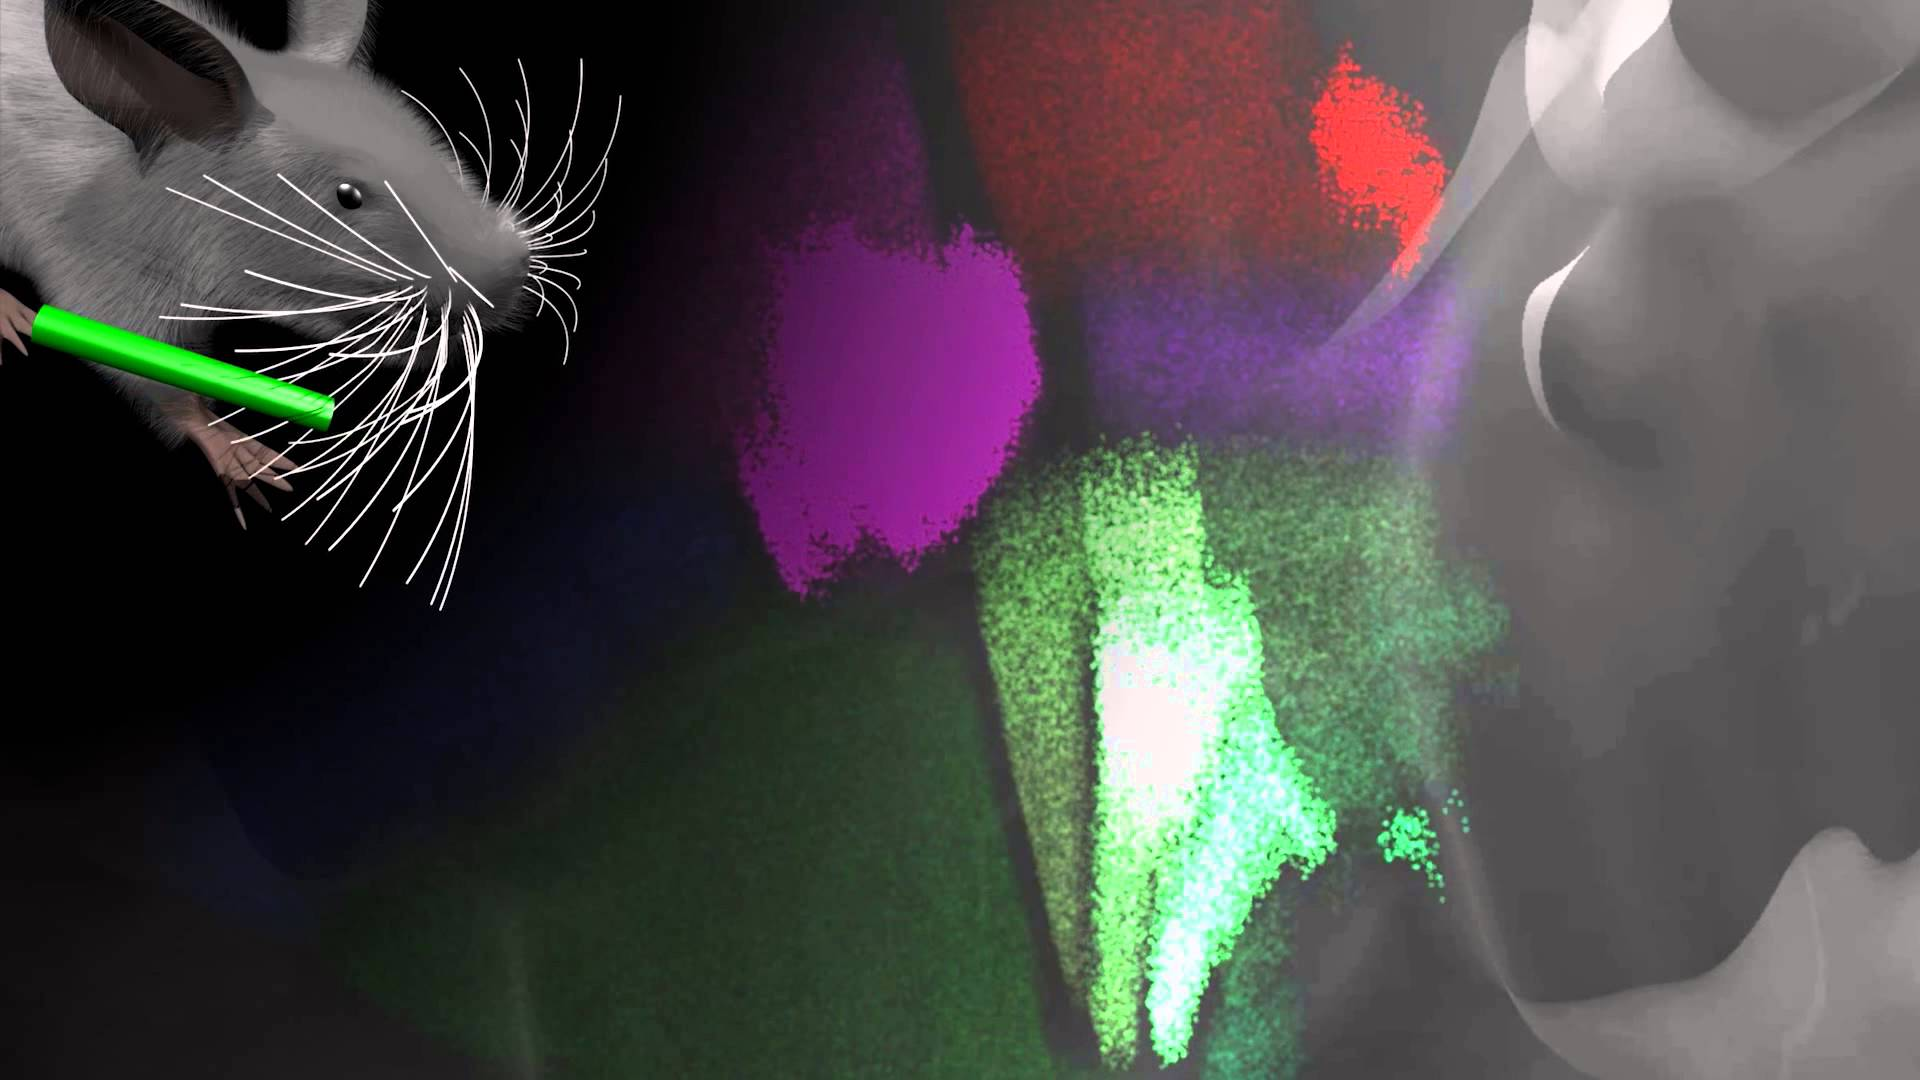
\includegraphics[width=0.6\textwidth]{virtualmouse}
	\caption[A virtual mouse's brain being stimulated(via the green rod)]{\centering \label{virtualmouse}A virtual mouse's brain being stimulated(via the green rod)\footnote{}}
	
\end{figure}
\footnotetext{https://www.youtube.com/watch?v=ldXEuUVkDuw[Accessed 01/04/2016]}
 They believe that in principle this could be repeated for the brain of any organism and it will continue to get more realistic and useful with time. If there were any doubts in our client's mind as to the likelihood of ever being able to use such a vast, complex amount of data, this should certainly help to dispel them. Other teams are working towards the same goal, in late 2015 the Blue Brain Project simulated 31 000 neurones in a similar fashion \cite{markram2015reconstruction}. More recently the Human Brain Project have released a set of virtual robots to which different brain models can be applied, such as a virtual mouse which can differentiate between colours. Whilst it may seem simplistic currently, plans to extend these models to physical robots suggest that our client's may not be confined to a virtual world but could also expect to return to a physical body. Over the duration of the project it would not be unreasonable to suggest further developments in computation will allow improved models to retrieve memories and recover a person's identity from the data we will provide.


\newpage
\pagestyle{plain}
\clearpage
\vspace*{\fill}
\centering
\begin{center}
	\begin{minipage}{.8\textwidth}
		
\textbf{With thanks to our tutors:}\newline
Frank Wood, Antoine Jerusalem and Jos\'{e} Mar\'{\i}a (Chema) Pe\~{n}a\newline
\\
\textbf{And our guest lecturers:}\newline
Narayanan (Bobby) Kasthuri, Jeff Lichtman, Will Roncal, Pascal Fua, Angel Merchan, Athanasios Tsanas, Aravindh Mahendran and Antonio LaTorre
	\end{minipage}
\end{center}
\vfill % equivalent to \vspace{\fill}
\clearpage

\newpage
	\pagestyle{plain}
	\bibliography{bib}
	\bibliographystyle{abbrv}

	
\end{document}

